\documentclass[11pt]{article}

\usepackage[utf8]{inputenc}
\usepackage{geometry}
\usepackage[pdftex]{graphicx}
\usepackage{tabularx}

%bib options
\usepackage[backend=bibtex,style=authoryear,natbib=true]{biblatex}
\addbibresource{Chap1.bib}

\usepackage{dsfont}
\usepackage{multirow}
\usepackage{amsmath,amsfonts,amssymb}
\usepackage{subcaption}

%hyperlinks options
\usepackage{hyperref}
\hypersetup{
    colorlinks=true,
    linkcolor=blue,
    filecolor=magenta,      
    urlcolor=cyan,
    citecolor=cyan
    }

 \geometry{
 a4paper,
 total={180mm,257mm},
 left=20mm,
 top=20mm,}
 
\title{Are historical stage records useful to decrease the uncertainty of FFA? A 200-year long case study}
\author{Mathieu LUCAS, Benjamin RENARD, Jérôme LE COZ, Michel LANG, Gilles PIERREFEU}

\begin{document}

\maketitle

\begin{abstract}

    This work proposes methods to make the most of long discharge series in flood frequency analysis, and provides insights on how historical data may or may not improve design floods estimates. Flood frequency analysis based on peak flow series from hydrometric stations is widely used to estimate flood hazard. The uncertainty around flood frequency estimates depends on sample size and on the uncertainty of streamflow data. Documentary evidence allow lengthening the continuous discharge series available and therefore has the potential to reduce sampling uncertainty. However, specific uncertainties affect those data as the stage/discharge relationship is generally difficult to estimate in this century-long context and as ancient visual stage reading were less frequent than recent sensor-measured stages. A consistent treatment of uncertainty over the whole data processing chain seems essential but is usually not performed. In the proposed approach, uncertainties are estimated and propagated from stage measurements to extreme flood quantiles estimates using Monte Carlo procedures. This allows exploring the role of both streamflow and sampling uncertainties in design floods estimations. This approached is applied to an exceptional 205-year long continuous discharge series of the Rhône River at Beaucaire. Results show that sampling uncertainty is reduced when sample size increases from 50 to 100 years, but is not much reduced beyond 100 years. However, the streamflow uncertainty contribution is increased when considering older and thus more uncertain floods. 

\end{abstract}

\section{Introduction}
    \paragraph{}
    Flood frequency analysis (FFA) is a widely used method to estimate flood hazard. It allows linking the magnitude of a flood to its probability of occurrence (\citet{hamed_flood_2019}; \citet{jain_design_2019}). Design floods, estimated for various exceedance probabilities (or equivalently, return periods), are commonly used for population safety policies, land use planning, as well as industrial safety. The most standard FFA approach is to estimate a distribution using a sample of flood peaks (typically, annual maximum discharges or discharges over a given threshold). Extrapolation of this distribution allows reaching the desired flood quantile that commonly corresponds to a 100 or 1000-year return period. 
    % refs FFA from FFA book ?
    
    \paragraph{}
    This FFA approach is affected by various sources of uncertainty. First, the hydrological data used to estimate the FFA distribution is uncertain: indeed, the usual process for deriving streamflow time series is going through steps that lead to measurement (gaugings and stage) and model (rating curve) errors. Moreover, the estimated FFA distribution is itself uncertain because of the limited size of the available streamflow data \citep{kjeldsen_uncertainty_2011}. Considering the decisions that rely on flood frequency analysis, a consistent treatment of uncertainty all over the data processing chain is essential but is usually not performed.
    % more references here again
    
    \paragraph{}
    Streamflow series are affected by several sources of uncertainty as described by \citet{mcmillan_benchmarking_2012} benchmark. First, stage measurements are affected by various sources of uncertainty. This uncertainty is often neglected but may have a important impact on the final hydrograph \citet{hamilton_quantifying_2012}, especially for historical stage series. A large number of stage error sources is identified in the literature (\citet{van_der_made_determination_1982}; \citet{petersen-overleir_uncertainty_2005}; \citet{mcmillan_benchmarking_2012}, \citet{horner_impact_2018}), such as staff gauge reading errors, levelling of the staff gauge, or stage sensor calibration. The frequency of measurement may also induce errors. With modern automatic systems, stage is measured with a time step generally smaller than the speed of variation of the stage (e.g. between 15 min and 1 hour), which leads to negligible errors. However, before the rise of automatic systems, measurements were made by operators who were reading the staff gauge less frequently (e.g. once or a few times per day), thus possibly missing the flood peak. This issue is particularly important when old series are used. To estimate the measurement frequency uncertainty, \citet{hamilton_quantifying_2012} and \citet{kuentz_hydrometrie_2014} analysed this situation by sub-sampling recent data for which sub-hourly measurements are available. This allows calculating the difference between the variable of interest (such as the daily maximum stage) derived from scarce data, and the same variable derived from high-frequency measurements. \citet{kuentz_hydrometrie_2014} applied the calculated bias to correct old stage series at a monthly time step. This correction aimed at taking into account the error due to the daily variability caused by snow melt during cold months. However, this type of correction have never been applied to peak stage correction during floods, especially in the case of long stage series.
    
    \paragraph{}
    Rating curve uncertainty is also a main issue when dealing with streamflow series. Transforming stage into discharge requires calibration data (gaugings) to establish the stage/discharge relationship. Gaugings uncertainty depends on the method used (\citet{lecoz_quantification_2014} and \citet{puechberty_charte_2017}). Moreover, the rating curve is also affected by uncertainties coming from the imperfection of the chosen model to represent the actual hydraulic configuration and from parameter estimation. Many methods have been proposed to quantify these uncertainties (\citet{petersen-overleir_bayesian_2009}; \citet{juston_rating_2014}; \citet{le_coz_combining_2014}; \citet{morlot_dynamic_2014}; \citet{coxon_novel_2015}; \citet{mcmillan_rating_2015}; \citet{mansanarez_rapid_2019}). A comparison of several of these methods has been recently proposed by \citet{kiang_comparison_2018}. Another important issue affecting streamflow data accuracy is rating changes. The stage/discharge relationship is frequently affected by changes coming from various origins that can be natural or anthropic, for instance: bed geometry evolution during floods or river works, aquatic vegetation growth and decay, ice sheets... A regular monitoring through gaugings is essential to detect those changes \citep{ibbitt_gauging_1987}, that can be transient or sudden. Several methods have been proposed to deal with rating changes: estimating rating curves on moving temporal windows (\citet{westerberg_stage-discharge_2011} and \citet{guerrero_temporal_2012}), computing as many rating curves as there are gaugings \citep{morlot_dynamic_2014}, exploring changes in the annual minimum stages \citep{lapuszek_methods_2015}, selecting 0.5-years return period discharge as a threshold for rating changes \citep{mcmillan_impacts_2010}... More recently, \citet{darienzo_detection_2021} proposed a method based on a recursive segmentation procedure, accounting for both gaugings and rating curve uncertainties. This method has a particular interest when dealing with ancient and thus uncertain gaugings. Following the detection of rating shifts, rating curves should be estimated for each stable sub-period. This task may not be straightforward, as the number of gaugings available within a sub-period is not always sufficient to properly estimate the stage/discharge relationship for the whole discharge range. A common way to address this problem is to artificially repeat some gaugings from other stability periods (\citet{mcmillan_benchmarking_2012}; \citet{puechberty_charte_2017}). \citet{mansanarez_shift_2019} proposed an alternative approach to deal with this issue. They developed a stage-period-discharge (SPD) model  where some parameters of the rating curve are allowed to vary across periods, while the others are supposed fixed. This method has the advantage of transferring information between periods to improve the rating curve estimation for all the stable stage/discharge periods, even when few gaugings are available.
    % propagation
    \paragraph{}
    Estimating sampling uncertainty in FFA is a well-established approach. Whatever the chosen distribution and estimation method, standard statistical procedures are available. However, these standard procedures only quantify sampling uncertainty, and do not consider uncertainties affecting the data. The literature review proposed in the previous paragraphs show that methods for quantifying individual sources of uncertainty (stage, rating curve and FFA distribution estimation) are available. However, the way all these uncertainties propagate through the FFA analysis chain has been less thoroughly studied. A few solutions have emerged to propagate uncertainties in stage time series through uncertain rating curves (Dymond1982, Herschy 1998, \citet{petersen-overleir_uncertainty_2005}), but they assume independent stage errors and therefore neglects systematic errors. \citet{horner_impact_2018} proposed a consistent method for the propagation of both sources of stage uncertainty through uncertain rating curves. Therefore, it is possible to infer the contribution of each source of uncertainty in streamflow data. \citet{petersen-overleir_accounting_2009}, \citet{steinbakk_propagation_2016}, and \citet{vieira_assessing_2022} performed an integrated analysis where the rating curve parameters and the flood frequency distribution are both estimated. All these studies highlighted the importance of considering rating curve uncertainty for design flood estimations and concluded that, under some conditions, accounting for rating curve uncertainty may notably widen the uncertainty intervals around flood quantiles. However, none of them considered both stage measurement errors and rating changes, which may constitute a major source of uncertainty for streamflow data. This is particularly the case when dealing with long streamflow series for which stage uncertainty is important and rating changes may have been missed. Their consideration in a flood frequency framework is therefore not avoidable. 
    Readers should note that the "historical data" term used in this paper refers to the use of ancient, systematic and steady stage measurements, by opposition to the use of punctual/censored flood evidences, prior to steady stage measurements. 
    
    \paragraph{}
    The following questions will be considered in this paper: 
    \begin{itemize}
        \item[1.] How to make the most of historical hydrometric data in flood frequency analysis while accounting for uncertainties at each step of the procedure ? 
        
        \item[2.] What is the contribution of each source of uncertainty to the final flood quantile uncertainty when historical data are taken into account ? 
        
        \item[3.] To what extent does enlarging streamflow samples by adding increasingly uncertain historical data improve flood quantiles estimation ? How are the relative contributions of sampling and streamflow uncertainties evolving with sample size ?
    \end{itemize}

    \paragraph{}
    This paper will illustrate the chained application of methods to quantify and propagate uncertainty from stage records (and their limited time resolution) and stage-discharge rating curves to the estimation of extreme flood quantiles. While most of these methods already exist, a key novelty of this work is their combination to provide an end-to-end evaluation of the  uncertainty affecting FFA estimations, from stage to flood quantiles. An original method to quantify the stage uncertainty stemming from infrequent readings is also proposed.

    The paper is organized as follows. First, the methodology for estimating uncertain streamflow series in a century-long context is presented (section 2.1). It goes through the detection of rating shifts (section 2.2), the estimation of rating curves (section 2.3), and the estimation and propagation of stage errors (section 2.4). Then, an approach to propagate streamflow uncertainty through the estimation of extreme flood quantiles is proposed (section 2.5). This procedure is illustrated through its application to the Beaucaire gauge on the Rhône River (section 3), for which official flood hazard assessments only used discharge series from 1920 \citep{rigaudiere_etude_2000}. The recent works of \citet{pichard_hydro-climatology_2017} and \citet{bard_actualisation_2018} allowed building a continuous discharge series from 1816 to the present time, which makes it the ideal case study for this procedure. The results of this application are presented in section 4, and they are discussed in section 5, where avenues for improvements are proposed.


\section{Uncertainty propagation chain for flood frequency analysis}
    % \subsection{Overview}
    
    The uncertainty propagation framework (figure \ref{fig:ChProp}) is a chain of uncertainty estimation methods. It starts with the basic hydrometric data: stage series and gaugings, and the final results are the flood quantiles with uncertainty propagated from each previous step of the procedure. This uncertainty propagation is achieved by Monte Carlo methods.
    
    \begin{figure}[h!]
        \centering
        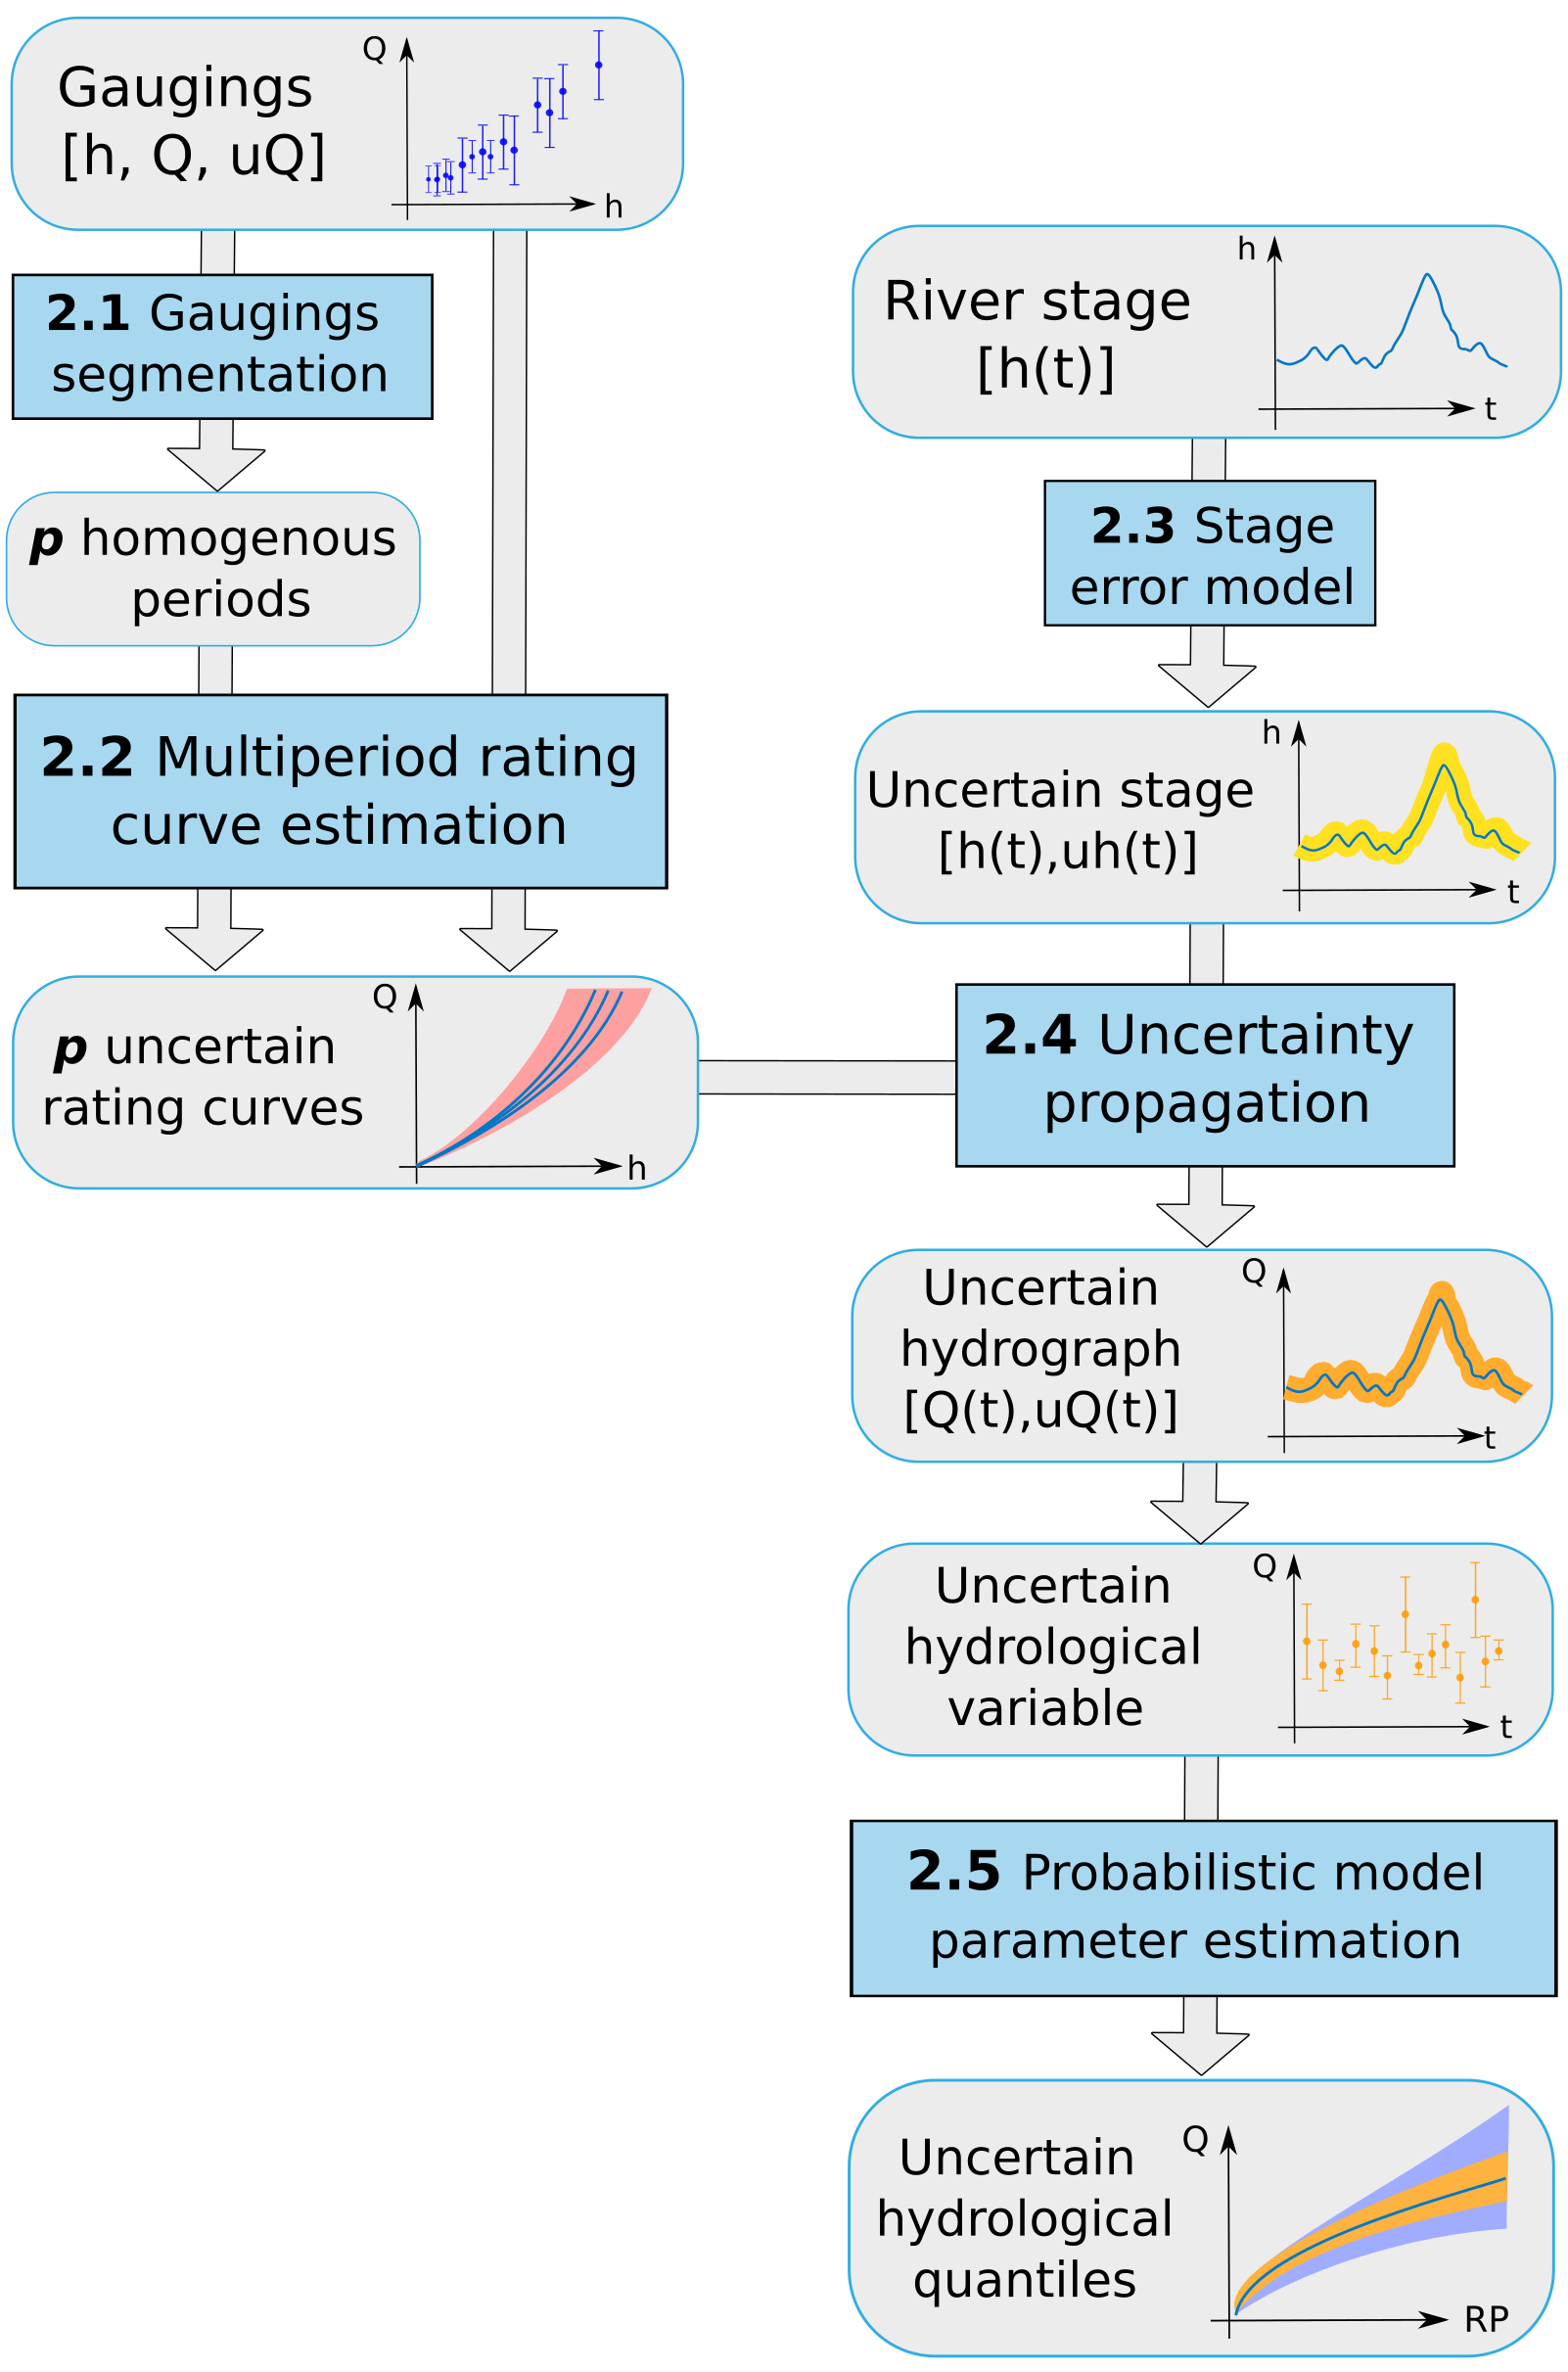
\includegraphics[width = 8cm]{Figs/1-uTotSchema.png}
        \caption{Block diagram of the uncertainty propagation procedure. Grey blocks represents data, blue blocks stands for analysis methods/models.}
        \label{fig:ChProp}
    \end{figure}
    
    The first three steps of the procedure rely on a rating curve estimation method. The BaRatin method \citep{le_coz_combining_2014} is used in this work. The Bayesian paradigm is used to estimate the parameters of the general rating curve equation, a combination of power equations: $Q = a(h-b)^c$, where Q is the discharge in m\textsuperscript{3}/s, the flow depth is the difference between the stage h (in m) and an offset b, and a and c being the coefficient and the exponent of the power function. The rating curve equation is deduced from a hydraulic analysis of the gauging station, aimed at identifying the main hydraulic controls governing the stage-discharge relation. The different controls can be activated successively or simultaneously. As an example, in a two-control hydraulic configuration, the rating curve $Q(h)$ may be expressed as: 
    
    \begin{itemize}
        \item $k_1 < h \leq k_2 $ (main channel): $Q(h) = a_1(h-b_1)^{c1}$
        \item $h \geq k_2$ (main channel + floodway):  $Q(h) = a_1(h-b_1)^{c1}+ a_2(h-b_2)^{c2}$
    \end{itemize}
    
    Parameters $a$, $b$ and $c$ can be linked with the physical properties of the control. For instance for a channel control with a wide rectangular cross-section, using a Manning-Strickler equation, we have: $a=KB\sqrt{S}$  ; $b=z$ ; $c=5/3$

    Bayesian inference allows deriving the posterior distribution of rating curve parameters by combining hydraulic information (priors for parameters of each hydraulic controls) and information from gaugings with uncertainty (likelihood). The posterior distribution is explored with a Markov Chain Monte Carlo (MCMC) sampler \citep{renard_application_2006}. Two sources of uncertainty are associated with the estimated rating curves. Parametric uncertainty reflects the uncertainty due to the rating curve parameters estimation because of the limited amount of gaugings and the gaugings uncertainty. Remnant uncertainty comes from the imperfection of the chosen rating curve model to represent the actual hydraulic configuration. We refer the reader to \citet{le_coz_combining_2014} for a more thorough description.


     \subsection{Rating shifts detection}
    
    The stage/discharge relationship is sensitive to sudden changes caused by morphogenic floods or other causes affecting the flow characteristics. Relying on residuals between gaugings and rating curve is the most common approach to monitor the stability of this relationship over time. The method proposed by \citet{darienzo_detection_2021} is used in this work. First, a baseline rating curve is estimated using the whole gaugings dataset. The residuals between gaugings and the rating curve are determined, and a statistical segmentation test is applied to those values. This segmentation procedure accounts for the residuals uncertainty, coming from both the gaugings and the rating curve uncertainties. The optimal number of segments is determined according the Bayesian Information criterion (BIC). Then, the same steps are applied recursively to each sub-period determined earlier. The recursive procedure is stopped when the BIC indicates that a single period is optimal. The advantage of this method is that both gaugings and rating-curve uncertainties are accounted for in a rigorous Bayesian framework. The results are not only the dates of rating-shifts but the posterior probability density function (pdf) of change point time. This allows affecting the shift time to the time of the maximum stage included in the posterior credibility interval. Prior knowledge is provided on the expected magnitude residuals, the number of segments at each iteration and the minimum time lag between two consecutive change points.
    %paramétrage et les options que tu retiens pour la suite de l'article
    
    \subsection{Multi-period rating curves estimation: stage-period-discharge model}
    
    \paragraph{}
    Once the stability periods have been identified, the next step is to estimate the rating curve associated with each period. \citet{mansanarez_shift_2019} developed a stage-period-discharge (SPD) model "based on the physical interpretation of changes in the stage-discharge relation across a series of stability periods". Prior knowledge is provided on the hydraulic controls and on the rating changes (i.e. estimated amplitude of change between the rating curves of two successive periods). In this model, some parameters of the rating curve equation are supposed to vary across the periods while the others do not. The BaRatin SPD method allows transferring information not only between periods, but also between controls, taking into account the uncertainty of both gaugings and of the rating curve model. This can be achieved without the need to artificially repeat gaugings across periods, which is of particular interest for stations with scarce gaugings. The identification of the potentially varying parameters is based on an hydraulic analysis of the site and and is an important step. Generally, changes are suspected coming from offsets or channel width parameters. The so-called local changes are supposed to affect the lowest control only (for instance the movement of the controlling riffle), whereas the global changes are affecting various controls at the same time (for instance, the scouring or filling of the channel, affecting low flows and main channel offsets at the same time). See \citet{mansanarez_shift_2019} for a detailed description of prior specification for time-varying rating curves. 
    
    \subsection{Stage uncertainties}
    \label{sec:StageErr}
    
    Many sources of error having distinct statistical properties can affect stage measurements, as described in \citet{horner_impact_2018}. Five different sources of uncertainty ($\delta_{1,...,5}$) affecting stage measurements are considered. Let $h(t)$ be the measured maximum stage of a day $t$. $\hbar(t)$, the unknown true maximum stage is assumed to be approximated by the following equation:
    
    \begin{equation}
        \hbar(t) = h(t) + \delta_1(t) + \delta_2(t) + \delta_3(t) + \delta_4(t) + \delta_5(t)
        \label{eq:StageError}
    \end{equation}
    
    For which: 
    \begin{itemize}
    
        \item[1 -]Staff gauge reading errors $\delta_1 \sim \mathcal{N}(0,\mu_1)$ originate from operators reading the gauge, where $\mu_1$ is depending on the precision of graduations (usually 1cm), and can be aggravated by the presence of waves, especially during floods \citep{mcmillan_benchmarking_2012}.

        \item[-]Most stage measurements nowadays are with automatic sensors of various types such as pressure sensors, floaters, radars, and they require a calibration to link the water stage to the measured proxy (respectively the pressure of the water column, the height of a floater, or the air draught). Two types of errors arise from this process: 
        \begin{itemize}
            \item[2 -] Sensor errors $\delta_2 \sim \mathcal{N}(0,\mu_2)$, where $\mu_2$ being usually estimated by the sensor constructor.
                
            \item[3 -] Sensor calibration errors $\delta_3 \sim \mathcal{N}(0,\mu_3)$ are related to the corrections made by operators when comparing the proxy measured by the sensor to the current stage at the staff gauge reference. An operator error at this step could affect the stage measurement until the next calibration. Sensor calibration error $\delta_3$ is hence constant between two calibrations and can be represented by drawing a new random value at each operator intervention.
        \end{itemize}
    
        \item[4 -]Datum errors $\delta_4  \sim \mathcal{N}(0,\mu_4)$ are related to changes in the datum reference measurement (usually the staff gauge zero value) and possible mismatches between successive gauges. Similarly to $\delta_3$, this error is constant between two gauge changes or datum reference measurements. 
    
        \item[5 -] Measurement frequency errors $\delta_5$ are related to the inadequacy of the frequency of measurement with respect to the speed of stage variations. As explained in the introduction, ancient stage measurements were done by operators who were reading the staff gauge much less frequently than modern automatic systems, which may lead to missing and hence underestimating the peak stage during floods. Unlike other types of stage errors, this error is hence necessarily positive, which calls for using a positive distribution such as the Log-normal or Exponential distribution at each measurement time-step. The parameters of this distribution can be estimated with data from the recent period, by analyzing the difference between the daily maximum stage derived from the high-frequency sensor measurement and that from an infrequent fixed-time reading. Note that the measurement frequency error for hourly (or less) measurements are considered negligible when considering large rivers with slow variations. 
   
    \end{itemize}
    
    \paragraph{}
    To sum up, $\delta_1$, $\delta_2$ and $\delta_5$ errors are drawn at each time step, while $\delta_3$ and $\delta_4$ errors are only drew at specific calibration times. $\delta_1$ to $\delta_4$ are assumed Gaussian with known standard deviations, while $\delta_5$ is assumed Exponential with parameter estimated by subsampling recent measurements. Monte Carlo methods are applied to combine these multiple uncertainty sources. The uncertainty around stage measurements from eq. \ref{eq:StageError} is hence represented by 500 possible realisations of the stage $h(t)$.
   
   \subsection{Propagation of stage and rating curve uncertainties to streamflow time series}
   
   Stage measurements realisations can be propagated through uncertain rating curves, following the approach described by \citet{horner_impact_2018}. To estimate the contribution of the different sources of streamflow uncertainties, four scenarii are considered:
   
   \begin{itemize}
       \item \textbf{Case 1: Maxpost streamflow.} Stage measurements are free of uncertainties and are assumed to be the median of the stage time series realisations. Rating curve estimation is also free of uncertainties. The unique stage time series is propagated trough the maxpost rating curves, resulting in one set of discharges time series. 
       \item \textbf{Case 2: Stage uncertainty.} Stage measurements are uncertain. This uncertainty is represented by $n$ possible stage time series, propagated through the maxpost rating curves. $n$ sets of discharge time series are obtained.
       \item \textbf{Case 3: Stage and parametric rating curve uncertainty.} Stage measurements are uncertain and rating curve estimation is affected by parametric uncertainties (represented by $m$ sets of rating curves) but is not affected by remnant uncertainties. The $n$ stage time series are propagated through $m$ sets of rating curves, leading to $n$ x $m$ sets of discharge time series. 
       \item \textbf{Case 4: Total streamflow uncertainty.} Stage measurements are uncertain and rating curve estimation is affected by both parametric and remnant uncertainties, represented by $m$ sets of rating curves. The $n$ stage time series are propagated through $m$ sets of rating curves, leading to $n$ x $m$ sets of discharge time series that represent the total streamflow uncertainty.
   \end{itemize}
   
    \subsection{Estimation of probabilistic model parameters and flood frequency analysis}
    \label{sec:STOODS}
    
    The Generalized Extreme Value (GEV) distribution is commonly used to model annual maximum discharges (AMAX) (see \citet{hamed_flood_2019} or \citet{jain_design_2019}). $\boldsymbol{\theta} = (\mu,\sigma,\xi)$ is the vector of GEV parameters: $\mu$ is the location parameter, $\sigma$ the scale parameter and $\xi$ the shape parameter. The parameters can be estimated based on an independent and identically distributed ($iid$) sample of $j$ annual maximum discharges (AMAX) $(\mathbf{q}_t)_{t=1,...,j}$. Bayesian-MCMC estimation is used in this work, as described in \citet{renard_application_2006}. The computed posterior distribution quantifies sampling uncertainty and is represented by $m$ MCMC-generated GEV parameters sets $\boldsymbol{\theta} = (\mu_{k=1,...,m},\sigma_{k=1,...,m},\xi_{k=1,...,m})$. The best set of parameters $\boldsymbol{\hat{\theta}}$ is the set that maximises the posterior distribution and is called "maxpost". 
    
    \paragraph{}
    As described in the previous sections, streamflow observations are affected by uncertainties. This streamflow uncertainty is represented by $n$ possible realisations of the AMAX series $q_t^{(i)}$. The final uncertain flood quantiles should thus consider both sampling and streamflow uncertainties. Similarly to \citet{steinbakk_propagation_2016}, the aim is to estimate the contribution of each source to the final/total uncertainty. For this purpose, three scenarii can be considered:
    
    \begin{itemize}
        % MP: median of stage err x maxpost RC x maxpost GEV
        \item \textbf{Case 1: Maxpost quantiles.} The series of AMAX floods $\mathbf{\hat{q}} = (\hat{q_t})_{t=1,...,j}$ is free of streamflow uncertainties and is obtained by propagating the median stage realisations through the maxpost rating curves. The GEV distribution is estimated using this single AMAX series, and the maxpost GEV parameters $\boldsymbol{\hat{\theta}} =  (\hat{\mu}, \hat{\sigma}, \hat{\xi})$. In this case, sampling uncertainties are not considered as well.
        
        % Hydro U: hydrometric U realisations x maxpost GEV
        \item \textbf{Case 2: Streamflow uncertainty}. AMAX floods are uncertain. This uncertainty is represented by $n$ sets of possible AMAX realisations: $\mathbf{q}^{(i)} = (q_t^{(i)})_{t=1,...,j;\quad i=1,...,n}$. Bayesian-MCMC estimation of the GEV distribution is performed $n$ times (one for each AMAX series) leading to $n$ x $m$ sets of GEV parameters. However, only the maxpost set of GEV parameters is computed on each AMAX flood realisation. This results in $n$ sets of GEV parameters $\boldsymbol{\hat{\theta}}^{(i)}_{i=1,...,n}$ that represent the effect of streamflow uncertainty of flood quantiles, ignoring sampling uncertainty.
    
        % Total U
        \item \textbf{Case 3: Total uncertainty.} AMAX floods are uncertain and sampling uncertainty is considered. Similarly to Case 2, Bayesian-MCMC estimation of the GEV distribution is performed $n$ times (one for each AMAX series) leading to $n$ x $m$ sets of GEV parameters. The result, reflecting both sampling and streamflow uncertainties, is thus represented by $n$ x $m$ sets of GEV parameters $(\boldsymbol{\theta}^{(i)}_k)_{k=1,...,m ; i=1,...,n}$.
    \end{itemize}
    
\section{Case study: The Rhône River at Beaucaire}

    \subsection{Site}
    
    The Rhône River at Beaucaire (95 590 km\textsuperscript{2}) is the most downstream gauge of the Rhône River (Figure \ref{fig:locstations}). It integrates all the complexity of the Rhône River hydrological regime, from the Alpine area to the French oceanic and Mediterranean influences. The annual mean discharge is around 1700m\textsuperscript{3}/s \citep{bard_actualisation_2018}, and the maximum known discharge reached 12 500m\textsuperscript{3}/s (May 1856, \citet{lang_les_2014}). The station lies in a flood sensitive area, as illustrated by the recent 2003 flood, resulting in 1.1 billion euros worth of damage \citep{lang_les_2014}. 
    The first stage measurements started in 1816, close to the bridge linking the cities of Beaucaire and Tarascon. This station is named "Pont de Beaucaire" (Kilometric point 267.6 from Lyon). Is has been used until the construction of the Vallabrègues hydroelectric system in 1967, which led to the derivation of a part of the discharge. Consequently, a new gauging station was installed 2 km downstream from the original one, downstream from the restitution of the deviated discharges. This station, logically named "Beaucaire Restitution" (Kilometric point 269.5), has been used ever since.

    \begin{figure}[h]
        \centering
        \includegraphics[width = 11cm]{Figs/2-BcrBv.png}
        \caption{The French Rhône River catchment and Beaucaire gauging stations}
        \label{fig:locstations}
    \end{figure}
    

        \subsection{Definition of rating curve equations and prior elicitation}
        \label{sec:prior_elicitation}
        \subsubsection{Pont de Beaucaire}
        
        Given historical cross-sections at Pont de Beaucaire (figure \ref{subfig:matrixCh}), the flow can be approximated by 2 additive hydraulic controls, for which the rating curve equation is the following:
        
        \begin{itemize}
            \item $k_1 < h \leq k_2 $ (main channel): $Q(h) = a_1(h-b_1)^{c1}$
            \item $h > k_2$ (main channel + floodway):  $Q(h) = a_1(h-b_1)^{c1}+ a_2(h-b_2)^{c2}$
        \end{itemize}
        
        \paragraph{}
        Within the main channel (when water stage is below $k_2 \approx$ 2m), the flow is splitted in two sub-channels since immemorial times (e.g. before 1816) as described by \citet{armand_ii_1907}. These sub-channels are communicating upstream and downstream from the gauge location, thus, they can be considered as a unique channel. The mobile sandbars that were separating the flow were progressively fixed by dikes to ease the navigation during XIX\textsuperscript{th} Century (figure \ref{subfig:diguesarmand}). The average width of this channel is the sum of both sub-channels widths ($\approx$ 300m).  
        At the gauge location, the floodway width is limited to 500m by unsubmersible levees  (figure \ref{subfig:matrixCh}), but is expanding several hundred meters downstream above $k_2$. This expansion is impacting the stage at the gauge. Consequently, the floodway rating curve is additive to the main channel. The floodway width is approximately 800m. 

       Parameters are derived from historical material retrieved in regional archives. This leads to the prior parametrisation described in table \ref{tab:PriorPt}. Physical parameters that have a direct hydraulic meaning are here expressed in the first three lines, then some of them are used to infer the $a$ parameter by using Monte Carlo propagation with a large number of samples of the physicals parameters ($B,K,S$). As recommended by \citet{le_coz_combining_2014}, log-normal priors are used for positive quantities such as slopes, channel widths and Strickler coefficients. Informative but imprecise priors are assigned to parameters such as channel widths, slopes or offsets which can be difficult to estimate precisely. For $c$ exponents, very precise priors are used because they depend on the control type (here $c=5/3$ for rectangular channel controls based on simplified Manning-Strickler equation). As recommended, structural uncertainty parameters have uninformative priors. According to historical profiles and cross sections, we assume that main channel and floodway offsets ($b_1$ and $b_2$) may have changed independently over time, but that main channel and floodway widths have not changed. As described by \citet{mansanarez_shift_2019}, this translates as offsets global and local changes $\delta_g$ and $\delta_l$. Those offsets changes on are computed as follows:
       
       \begin{itemize}
            \item $b_1^{(k)} = b_1^{(k-1)}-(\delta_g^{(k)}+\delta_l^{(k)})$ (incremental changes in the main channel)
            \item $b_2^{(k)} = b_2^{(k-1)}-\delta_g^{(k)}$ (incremental changes in the floodway)
       \end{itemize}
       
       As the most recent stable stage/discharge period obtained by gaugins segmentation is assumed to be the most known, it is used as the reference period. Changes are cumulative, and are therefore computed by respect to this reference period. Priors distributions of offset changes are determined in section \ref{sec:stageevolution}.
       
    %   \begin{align}
    %   \left\{\begin{matrix}
    %     &b_1^{(k)} = b_1^{(k-1)}-(\delta_g^{(k)}+\delta_l^{(k)}) \textrm{    (incremental changes in main channel)}  \\ 
    %     &b_2^{(k)} = b_2^{(k-1)}-\delta_g^{(k)} \textrm{    (incremental changes in the floodway)}
    %     \end{matrix}\right.
    %     \end{align}
       

        \begin{figure}[h!]
            \centering
            \begin{subfigure}{0.7\linewidth}
            \centering
            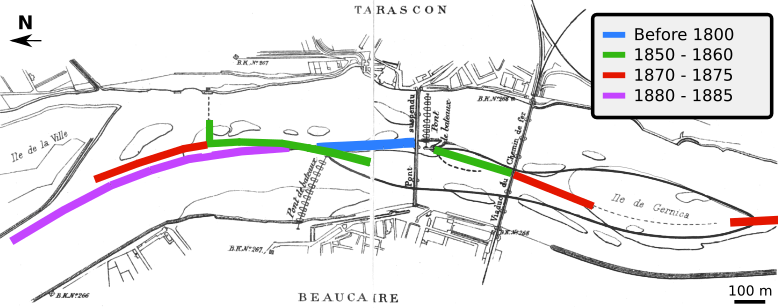
\includegraphics[width=1\linewidth]{Figs/3a-DiguesArmand.png}\hfill
            \caption{}
            \label{subfig:diguesarmand}
            \end{subfigure}
            
            \begin{subfigure}{0.6\linewidth}
            \centering
            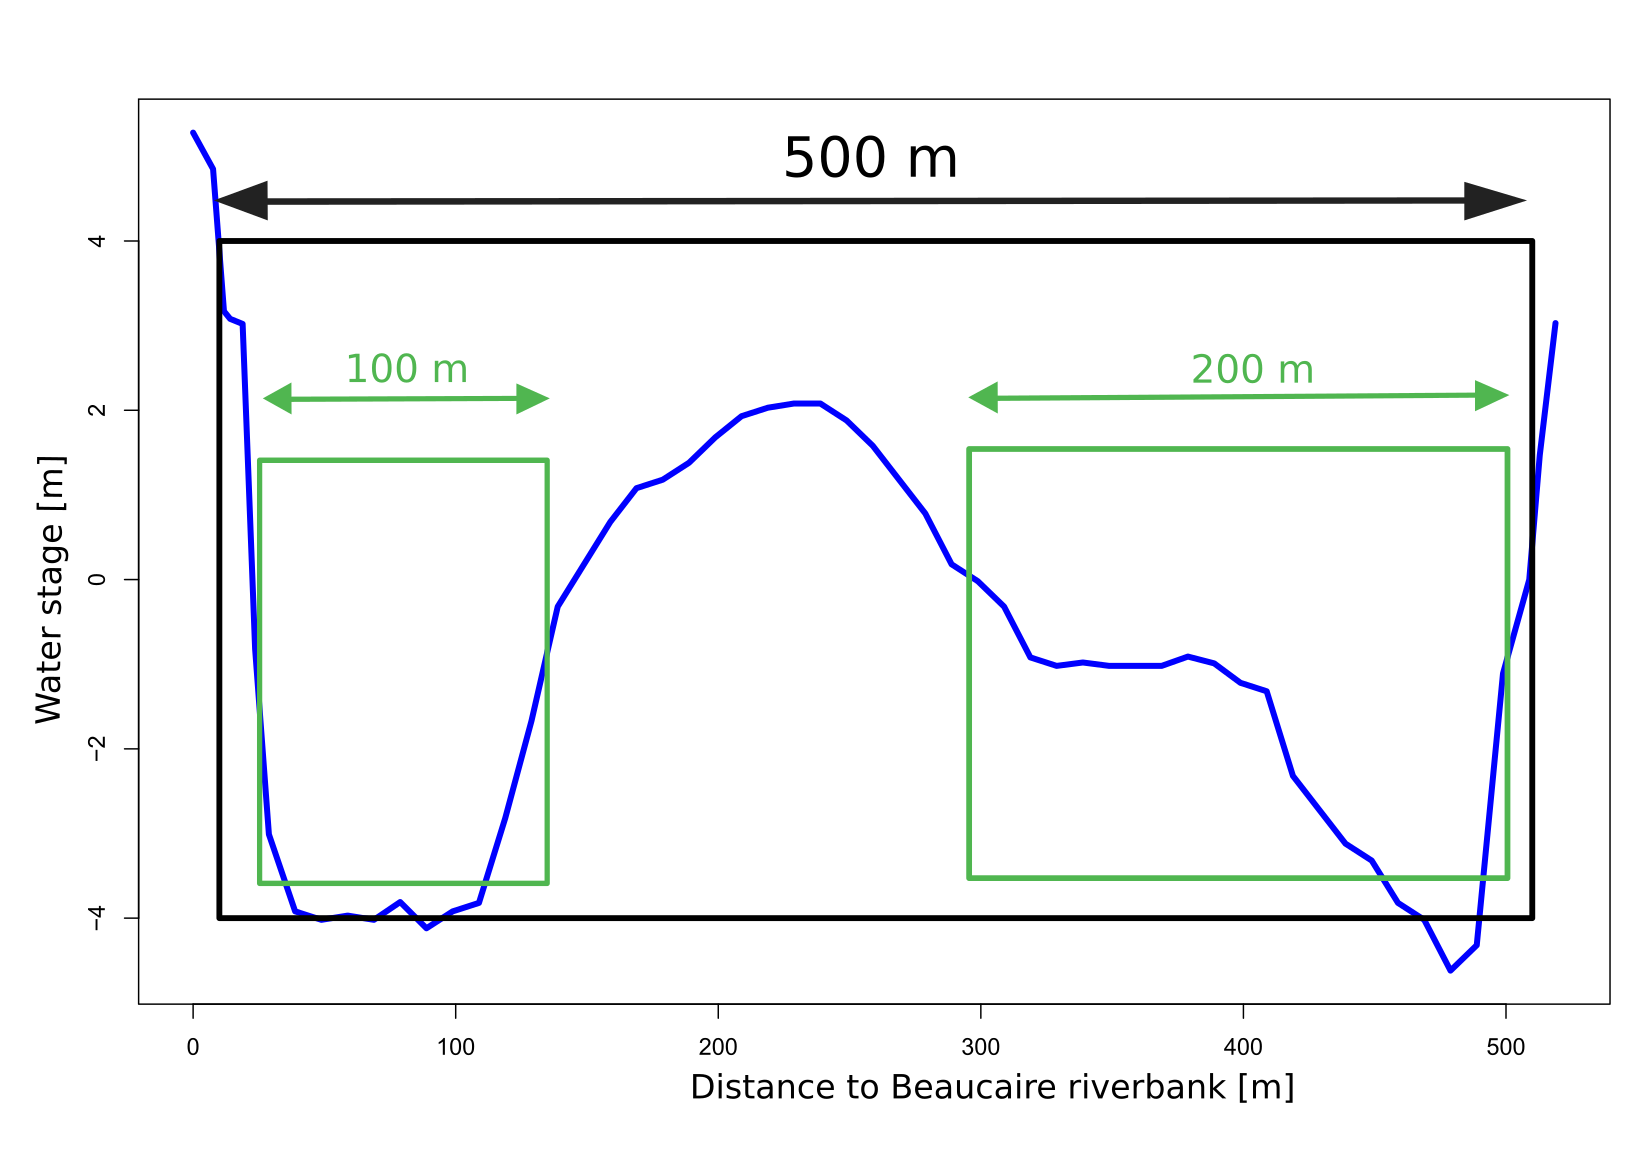
\includegraphics[width=1\linewidth]{Figs/3b-MatrixChenal_EN.png}
            \caption{}
            \label{subfig:matrixCh}
            \end{subfigure}
            
            \begin{subfigure}{.9\linewidth}
            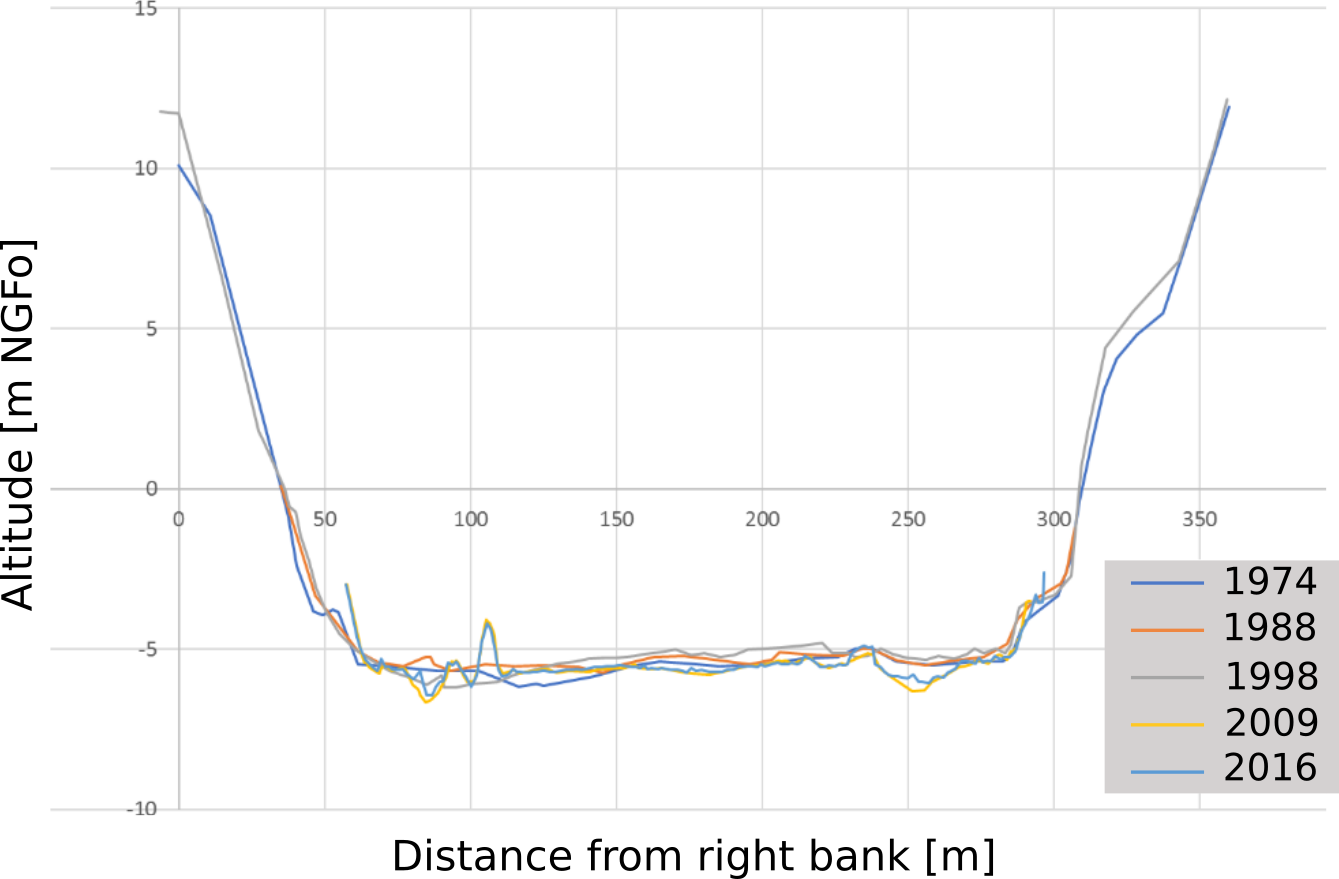
\includegraphics[width=.48\linewidth]{Figs/3c-ProfilsBardRestit.png}
            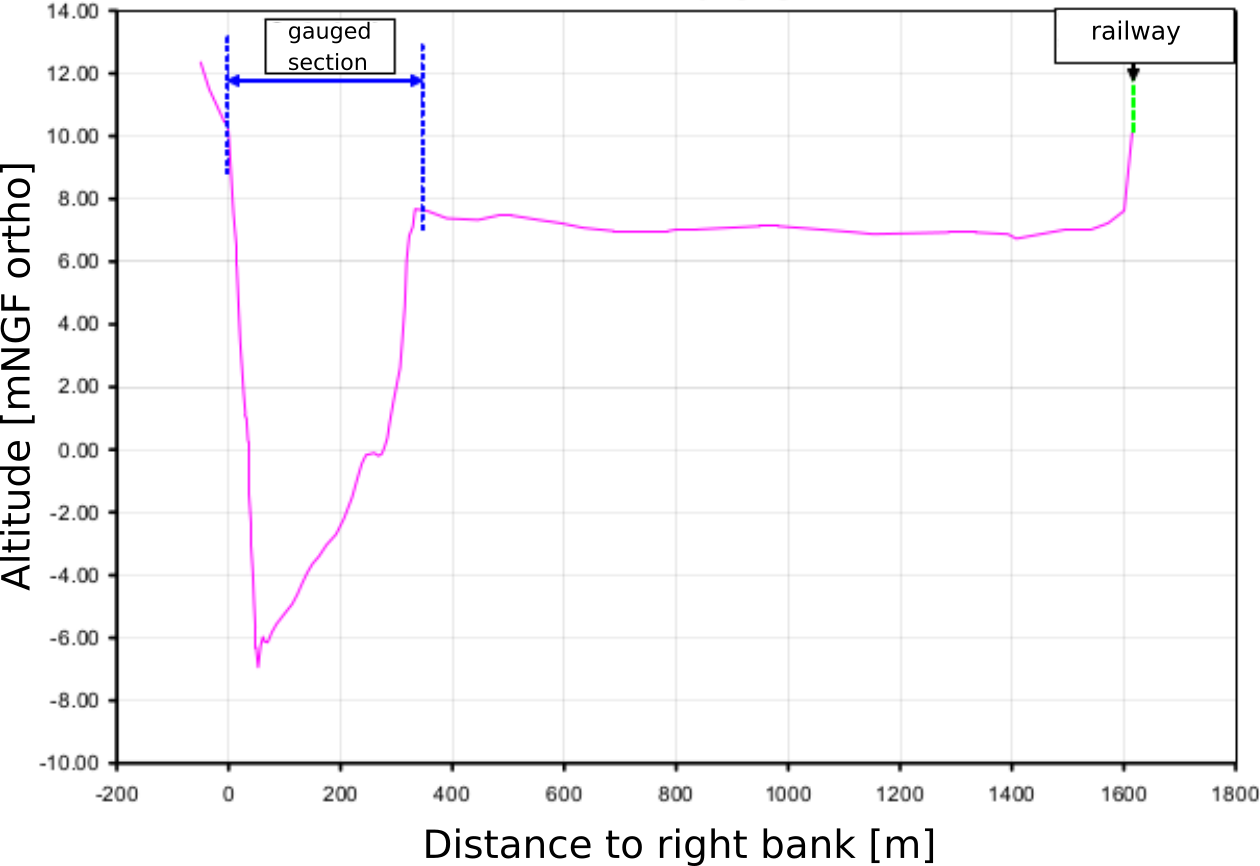
\includegraphics[width=.48\linewidth]{Figs/3c-ProfilAvalRestitEN.png}
            \caption{}
            \label{subfig:avalprofilesRestit}
            \end{subfigure}
            
            \caption{(a) Map of dike evolution in Beaucaire between 18\textsuperscript{th} and 20\textsuperscript{th} centuries, adapted from \citet{armand_ii_1907}; (b) Approximation of channel widths at Pont de Beaucaire station, based on a 1845 cross section; (c) Profiles from 1974 to 2016 (left) at Beaucaire Restitution station and 2.5km downstream from the station (right) from CNR data, freely translated from \citet{bard_actualisation_2018} and \citet{medd_debit_2005}}
            \label{fig:groupPriorPt}
        \end{figure}


        \subsubsection{Beaucaire Restitution}
        
        Beaucaire Restitution station have a more stable profile than Pont de Beaucaire according to 1974-2016 cross-sections (figure \ref{subfig:avalprofilesRestit} left) as there are no mobile sandbars separating the flow. The flow is approximated by a 3-controls configuration:
        
        \begin{itemize}
            \item $k_1 < h \leq k_2 $ (low flows): $Q(h) = a_1(h-b_1)^{c1}$
            \item $k_2 < h \leq k_3 $ (main channel): $Q(h) = a_2(h-b_2)^{c2}$
            \item $h > k_3$ (main channel + floodway):  $Q(h) = a_2(h-b_2)^{c2}+ a_3(h-b_3)^{c3}$
        \end{itemize}
        
        The very low flows (first control) are know to be influenced by the Mediterranean Sea level variations (approximately below 0m at the gauge). The first control is replaced by the second one when the stage is no longer influenced by sea level variations. At the gauge location, the 12m banks are preventing overflows (figure \ref{subfig:avalprofilesRestit} left). However, downstream from the station location, overflows are occurring at the left bank above approximately 8m (figure \ref{subfig:avalprofilesRestit} right). A floodway control, additive to the main channel, is representing those overbank flows. Low flows $b_1$ and main channel $b_2$ offsets are assumed changing over time, whereas floodway offset $b_3$ and channel widths are supposed constant. Priors of incremental changes are computed similarly to Pont de Beaucaire in the previous paragraph and are specified in section \ref{sec:stageevolution} results.
        
    \subsection{Stage series}

    \subsubsection{Pont de Beaucaire}
    
    Thanks to the archival work of \citet{pichard_hydro-climatology_2017}, a continuous stage series is available at Pont de Beaucaire from 1816 to 1967: daily time-step from 1816 to 1840, and three stages/day from 1841 to 1967. The records were made visually by an operator, at noon during the first years, then at 7AM, 12AM and 5PM (Figure \ref{fig:TabObsPt}). When three stages/day are available, the maximum of the three stages is considered as the daily maximum stage, and the unique value at noon as the daily maximum stage before 1840. Additionally, after 1840, when the stage was rising above 5m, the operators were making more frequent visual records (supposedly hourly measurements). When these records are available, they are of course used as daily maximum stages. Annual maximum stages are considered here, as this work is focused on floods. 
    
        \begin{figure}[h]
            \centering
            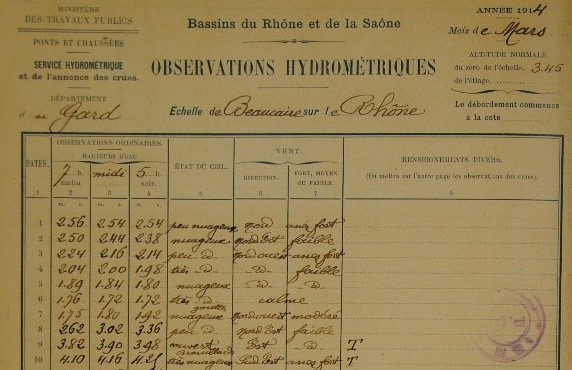
\includegraphics[width = 10cm]{Figs/4-TabObsBcrSmall.jpg}
            \caption{Table of limnimetric surveys at Pont de Beaucaire, March 1914. Operators were supposed to provide the water level at 7AM, 12AM and 5PM, as well as a few meteorologic details. (Departmental archives of Gard, 1914)}
            \label{fig:TabObsPt}
        \end{figure}
        
    Stages uncertainties are dependant on the measurement method, as described in \ref{sec:StageErr}. Table \ref{tab:StageErr} is summarizing the different sources of uncertainties at Beaucaire, they are detailed here as standard deviations $\mu$:
    
    \begin{itemize}
    
        \item Staff gauge reading uncertainty $\mu_1$ is taken as 5cm. Staff gauge precision is centimetric, but as this work is focused on floods, the error is expanded because of the waves that may complicate the reading. 
        
        \item Sensor precision $\mu_2$ and sensor calibration uncertainties $\mu_3$ are not considered at Pont de Beaucaire as the stage was read by operators directly on the staff gauge.
        
        \item \citet{bard_actualisation_2018} have compiled several elevation measurements of the datum reference. Most of those measurements occurred after the abandonment of Pont de Beaucaire station in favour of Beaucaire Restitution. Datum reference uncertainty $\mu_4$ is assumed to be equal to the standard deviation of those measurements: 6cm. The datum reverence measurement frequency during the exploitation of Pont de Beaucaire station is assumed to be 25 years. Hence, the datum reference uncertainty is drawn every 25 years.
        
        \item As described in section \ref{sec:StageErr}, the distribution of measurement frequency errors $\delta_5$ can be estimated using the frequent stage measurements at Beaucaire Restitution between 1970 and 2020 (50 AMAX values). For the "one stage/day" case (mimicking the 1816-1840 period), this error is corresponding to the difference between the maximum hourly stage value and the stage at noon of the same day. The "three stages/day" error is the difference between the maximum hourly stage of a day, and the maximum of 7AM, noon and 5PM stages of the same day. At Beaucaire Restitution, the one stage/day error maximum value is 2.2m, and the three stages/day error value is 0.9m. An exponential distribution is fitted for both errors samples and is used to correct the annual maximum stages at Pont de Beaucaire. According to CNR staff gauge management instructions, after 1840 and for the stages above 5 meters, hourly measurements were made by observers. Hence, measurement frequency error $\delta_5$ can be considered as negligible when stage is above 5 meters after 1840. 
    \end{itemize}

    \paragraph{}
        \citet{symadrem_programme_2012}, \citet{pichard_hauteurs_2013} and \citet{bard_actualisation_2018} suggested that for the floods during which dike breaks happened downstream from Beaucaire, stage measurements should be corrected because the stage measured at the station may lead to underestimate the actual discharge of the flood. The stage corrections for the more thouroughly studied floods of 1840, 1841 and 1856 estimated by \citet{symadrem_programme_2012} are adopted. The stage uncertainty of these floods is replacing the previously estimated uncertainty and is assumed Gaussian, with mean the estimated discharge and standard deviation 
        half of the applied correction, chronologically: 0.94, 0.4 and 0.4m. 

    \subsubsection{Beaucaire Restitution}
    
    For Beaucaire Restitution station, most of the stage uncertainty values are coming from \citet{cetiat_conference_2005} expertise on behalf of Compagnie Nationale du Rhône. They are summarized in table \ref{tab:StageErr} and detailed here:
    
    \begin{itemize}
    
        \item Staff gauge reading uncertainty is considered null as the measurements are done by automatic sensors. However, gauge reading uncertainties are affecting sensor calibration uncertainties $\mu_3$. 
        
        \item Instrument precision uncertainty : $\mu_2 = 0.01/\sqrt{3}m$ is coming from the sensor constructor specifications.
        
        \item The standard deviation of all the re-calibrations realized by the operators is equal to 5cm according to \citet{cetiat_conference_2005}. Calibration is also affected by staff gauge reading uncertainties, because the stage read in the staff gauge is the reference used by operators to calibrate the sensor. \citet{cetiat_conference_2005} estimated a 3.35cm uncertainty for the gauge reading uncertainty. Therefore, gauge reading and calibration uncertainties are combined as follows: $\mu_3 = \sqrt{0.0335^2 + 0.05^2} = 0.06m $. As the average time lag between calibration is 6 months, a new value of $\mu_3$ is drawn for each annual maximum stage. 
        
        \item Datum reference uncertainty $\mu_4$ is considered negligible because of the precision of modern topographic measurements.
        
        \item Measurement frequency uncertainty $\mu_5$ is considered negligible, because the sub-hourly measurement frequency is assumed adequate to capture the Rhône River stage variability. 
        
    \end{itemize}

    \begin{table}[h]
    \centering
    \resizebox{\columnwidth}{!}{%
    \begin{tabular}[c]{|c|c|c|c|c|cc|}
    \hline
    \multirow{2}{*}{\textbf{Date}} &
      \multirow{2}{*}{\textbf{\begin{tabular}[c]{@{}c@{}}$\boldsymbol{\delta_1}$: gauge\\ reading\end{tabular}}} &
      \multirow{2}{*}{\textbf{\begin{tabular}[c]{@{}c@{}}$\boldsymbol{\delta_2}$: instr.  \\ precision\end{tabular}}} &
      \multirow{2}{*}{\textbf{\begin{tabular}[c]{@{}c@{}}$\boldsymbol{\delta_3}$: sensor\\ calibration\end{tabular}}} &
      \multirow{2}{*}{\textbf{\begin{tabular}[c]{@{}c@{}}$\boldsymbol{\delta_4}$: datum\\ reference\end{tabular}}} &
      \multicolumn{2}{c|}{\textbf{\begin{tabular}[c]{@{}c@{}}$\boldsymbol{\delta_5}$:\\ measurement frequency\end{tabular}}} \\ \cline{6-7} 
     &
       &
       &
       &
       &
      \multicolumn{1}{c|}{\textbf{Stage\textless5m}} &
      \textbf{Stage$\geq$5m} \\ \hline
    \textbf{Before 1840} &
       $\mathcal{N}(0,0.05)$ &
      - &
      - &
       $\mathcal{N}(0,0.06)$ &
      \multicolumn{2}{c|}{$\exp(2.18)$} \\ \hline
    \textbf{1840 - 1967} &
      $\mathcal{N}(0,0.05)$ &
      - &
      - &
       $\mathcal{N}(0,0.06)$ &
      \multicolumn{1}{c|}{\begin{tabular}[c]{@{}c@{}}$\exp(8.86)$\end{tabular}} &
      - \\ \hline
    \textbf{1970 - 2020} &
       - &
       $\mathcal{N}(0, 0.01/\sqrt{3})$ &
       $\mathcal{N}(0,0.06)$ &
      - &
      \multicolumn{2}{c|}{-} \\ \hline
    \end{tabular}%
    }
    \caption{Distributions used for the different sources of stage errors (in meters)}
    \label{tab:StageErr}
    \end{table}
        
    \subsection{Gaugings}

    \paragraph{}
    244 gaugings were retrieved at Pont de Beaucaire, from 1840 to 1967. After excluding a few gaugings which were considered doubtful, 233 measurements are remaining. The frequency of gaugings is variable in time. No gaugings were retrieved before 1840 and there are a few 10 to 20 years gaps without gaugings, which makes the estimation of the stage/discharge relationship over time challenging. The uncertainty of the gaugings at Beaucaire depends on the gauging method, as specified in table \ref{TabIcJau}.
    
    \paragraph{}    
    304 gaugings were available at Beaucaire Restitution. A few of these were out of the period of stage measurements availability and were discarded. Finally, 296 gaugings were selected. As modern hydrometric developments allowed estimating the uncertainty for each individual gauging (particularly for ADCP and current meters), those values are used when available in the CNR archives. If not, values from table \ref{TabIcJau} are considered. 
        
         \begin{table}[ht]
            \centering
                \begin{tabular}{| l | l |} 
                        \hline
                        \textbf{Gauging method} & \textbf{Uncertainty standard deviation} \\
                        \hline
                        Current meter at 0.6 h and surface & 5\% \\
                        \hline
                        Current meter point by point & 3.5\% \\
                        \hline
                        Surface current meter & 7.5\% \\
                        \hline
                        Unknown type & 7.5\% \\
                        \hline
                        ADCP & 3.5\% \\
                        \hline
                        Floats before 1936 & 10\% \\
                        \hline
                        Hydrotachymeter before 1936 & 10\%\\
                        \hline
                \end{tabular}
            \caption{Gaugings uncertainty depending on the method used (hypotheses from \citet{bard_actualisation_2018}). Expressed as standard deviations of the measured discharge in \%.}
            \label{TabIcJau}
        \end{table}
 
 \section{Results}
 
    \subsection{Assessment of rating shifts}
    
    \subsubsection{Low flows stages evolution}
    \label{sec:stageevolution}
    
    One way to follow the evolution of riverbed elevation and to help specifying priors for rating curve vertical evolution is to study the long-term evolution of the yearly lowest stages, as described by \citet{lapuszek_methods_2015}. This analysis has to be carried out carefully, as the analysed variable is not only informing on the channel evolution, but also on the hydrologic and climatic variability. Here, the 5\% annual quantile is used (figure  \ref{fig:quantile5_both}). At Pont de Beaucaire (1816 - 1967), the 5\% quantile is oscillating with a 0.3m standard deviation. Those variations do not seem related to the occurrences of majors floods. The prior distributions of local and global offsets changes defined in section \ref{sec:prior_elicitation} are assumed Gaussian and equal to 0.3: $\delta_g^{(k)} = \delta_l^{(k)} \sim \mathcal{N}(0,0.3)$ (see table \ref{tab:PriorPt}).
    
    At Beaucaire Restitution (1970-2020), the annual 5\% quantile shows a large decrease during the first 4 years (more than 1m). This is a consequence of Vallabrèges hydraulic works between 1967 and 1970 as well as the important dredging just after the beginning of the system exploitation. A geomorphologic readjustment after the works in the channel may as well have affected the riverbed level. After these first years, the channel bottom is stabilized but there is a slight scouring trend of about 30cm in 40 years. Beaucaire Restitution 5\% quantiles standard deviation reaches 0.5m. Prior standard deviation of local changes is assumed larger than 0.5m and therefore defined as 0.8m to be more representative of the large changes that occurred during the first years: $\delta_l^(k) = \mathcal{N}(0,0.8)$. Standard deviation of prior global changes is assumed equal to 0.3m to represent the scouring trend in the main channel: $\delta_g^{(k)} = \mathcal{N}(0,0.3)$ (see table \ref{tab:PriorRestit}).
    
    \begin{figure}[h]
        \centering
        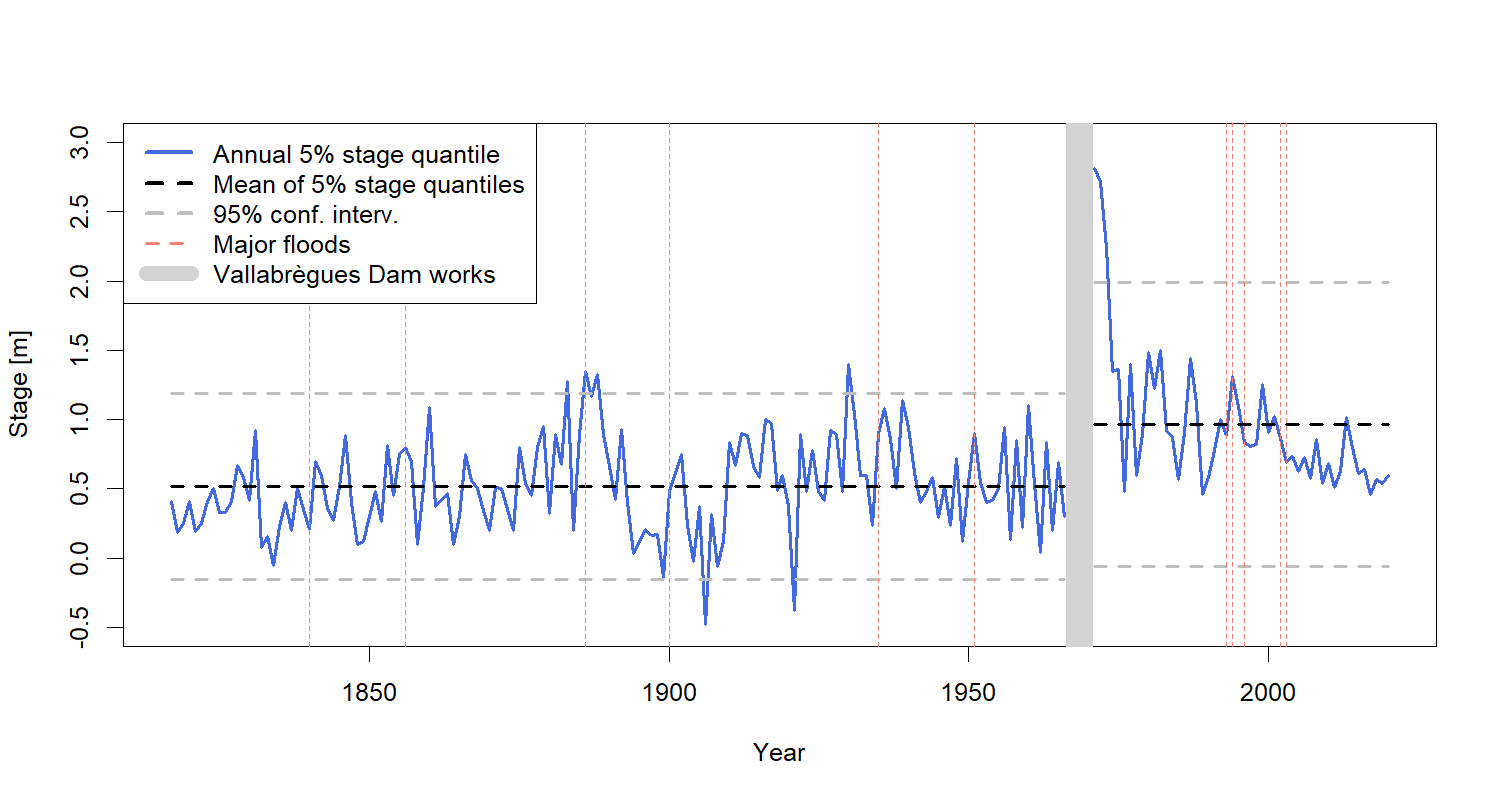
\includegraphics[width = 12cm]{Figs/5-Quant5perc_both.png}
        \caption{Time series of annual 5\% stage quantile of both Pont de Beaucaire (1816-1967) and Beaucaire Restitution (1970-2020) stations used to specify priors on rating shift parameters.}
        \label{fig:quantile5_both}
    \end{figure}
   
    \subsubsection{Gaugings segmentation}

    \citet{darienzo_detection_2021} segmentation procedure is applied at Beaucaire (Figure \ref{fig:SegmBoth}). The expected order of magnitude of rating curve residuals is assumed Gaussian with zero mean and a 500m\textsuperscript{3}/s standard deviation for both stations. The maximum number of segments at each iteration had been fixed at six (see \citet{darienzo_detection_2021} for details on priors and parameters specification).

    \begin{figure}[h!]
        \centering
        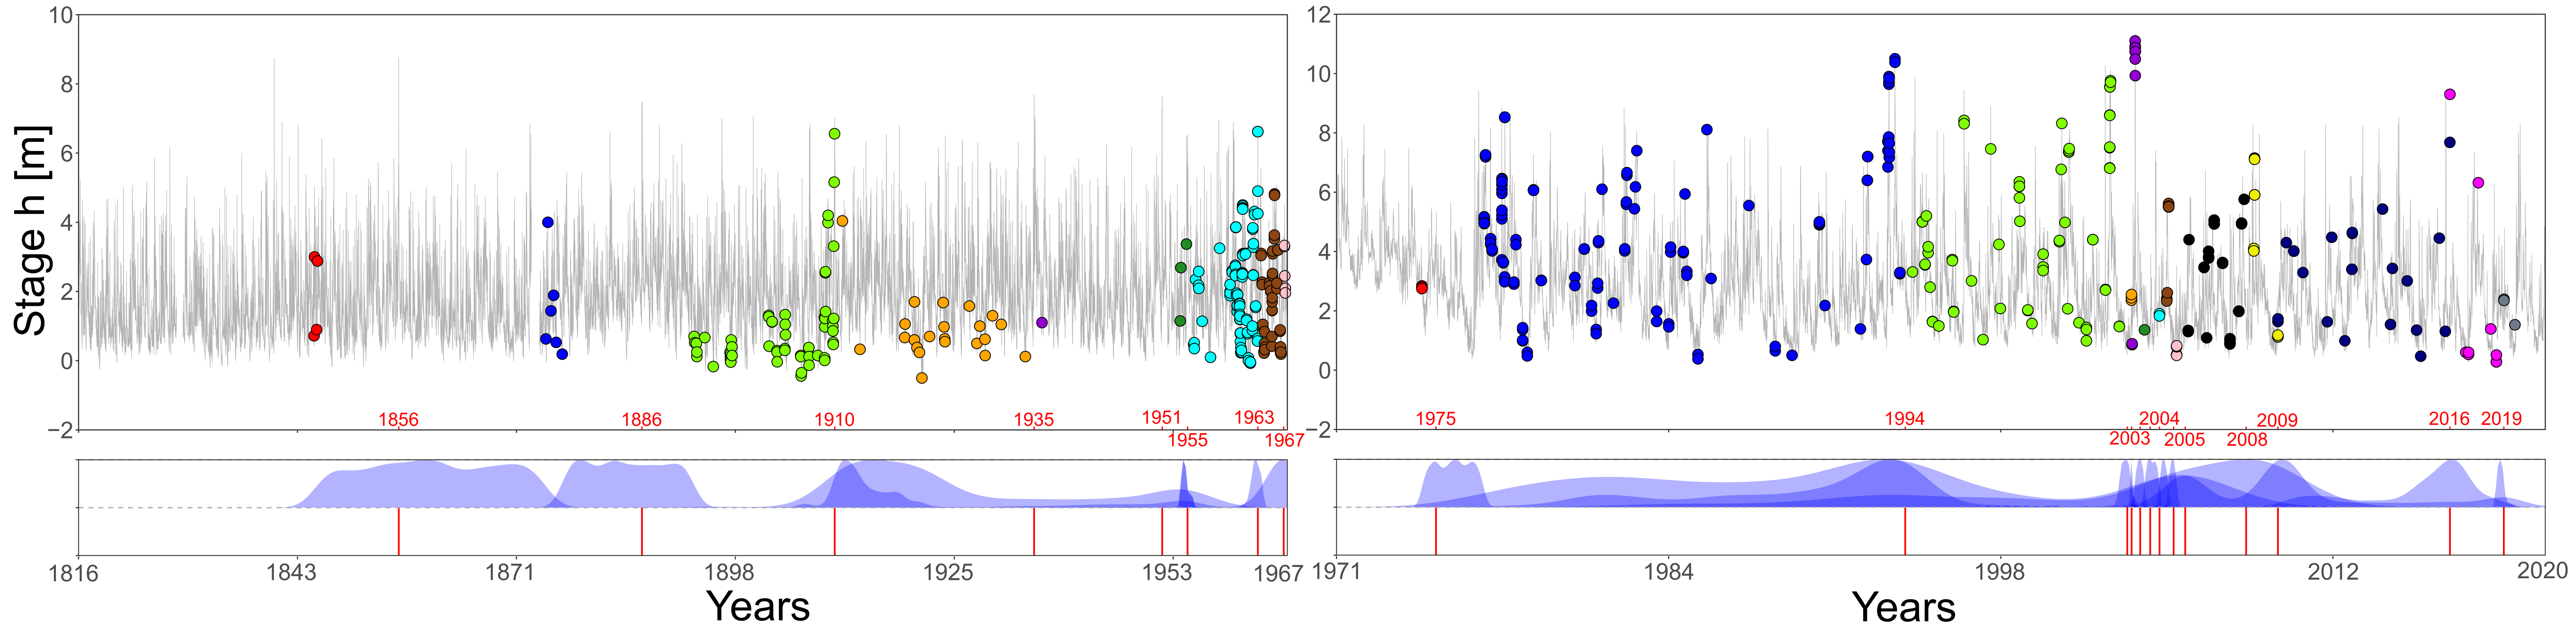
\includegraphics[width =1\linewidth]{Figs/6-SegmBoth.png}
        \caption{Gaugings segmentation of the Rhône River at Pont de Beaucaire (left) and Beaucaire Restitution (right). Dots represents gaugings with different colors for each stability period. The grey curve is the stage series. Blue ribbons represents posterior pdf of shift times and red segments are the retained shift times taken as the maximum stage included in each posterior pdf interval.}
        \label{fig:SegmBoth}
    \end{figure}
    
    \paragraph{}
    Eight shift times are detected at Pont de Beaucaire (left), located at the date of the largest flood within posterior pdfs. The gauging frequency is erratic through the history of the station and some periods include a small number of gaugings. As a consequence, the posterior pdfs of shift times span many years for the first shifts, and are similar to uniform distributions between sets of gaugings. This is reassuring about the method since there is indeed no information during long no-gauging periods to identify a shift time. It is no surprise that most of the shifts occur very close to the largest historical floods. 1935 and 1951 time shifts are respectively corresponding to the 3\textsuperscript{rd} and 4\textsuperscript{th} most important floods of the history of the station. There is, by construction of the segmentation model, no shift before 1845, year of the first available gaugings. However, we can consider that 1840 flood (supposedly the largest flood since 1800) is likely to have caused a shift. Therefore, we consider an additional shift time at the exact flood date. This brings the total number of stability periods to 10 (see detailed dates in table \ref{tab:ShiftDates}). 
    
    \paragraph{}    
    Thirteen shift times are detected at Beaucaire Restitution. As can be seen in figure \ref{fig:SegmBoth} (right), gauging frequency is far larger than for Pont de Beaucaire station (except during the 5 first years), allowing a better determination of the rating shift times. 
    Due to the lack of gaugings at the beginning of the series, only one rating shift is detected but many shifts potentially took place in those first four years as morphological readjustments and dredging occurred (see previous section). This first shift is assumed to be located to the first important flood of the station in 1976, after which the channel is stabilized. The following shift occurred during 1994 flood, one of the most important of the station. The most notable flood at Beaucaire Restitution occurred in 2003 (11 500m\textsuperscript{3}/s, with a return period about 100 years according to \citet{medd_debit_2005}). Unsurprisingly, the stage/discharge relationship is considerably disrupted by this event, as reflected by the six rating shifts detected from 2003 to 2005. Two out of these six shifts were discarded because the shift amplitude is considered minor based on further analysis of the corresponding rating curve change. The largest flood within posterior pdf of those floods is almost always corresponding to the 2003 flood. This is also the case for 2005, 2008 and 2009 shifts, for which the posterior pdf spans many years and include 2003 flood. Therefore, the shift dates are assumed to be located to the maxpost shift times, as several shifts can not be located at the same date. Lastly, the last shift of 2019 is also discarded because the shift amplitude is considered minor based on further analysis. Finally, ten rating shifts were retained. This brings the number of stability periods to eleven for Beaucaire Restitution, as seen in table \ref{tab:ShiftDates}. 
        
    \subsection{Multiperiod rating curves estimation}

    \paragraph{}
    Uncertain rating curves are estimated using \citet{mansanarez_shift_2019} model, based on gaugings segmentation stability periods. This leads to ten rating curves for Pont de Beaucaire (figure \ref{subfig:RcPt}), that show a good adequacy with gaugings. The widest uncertainty interval for low discharges belongs to the first period (1816-1840: dark red) for which no gaugings are available. The most important rating change arise between periods two and three, and is probably related to channel works for navigation and to the 1856 great flood consequences. After this phase of changes, the stage/discharge relationship stabilizes, along with a slow increase the offsets, which may be a consequence to the filling of the channel noticed in figure \ref{fig:quantile5_both}. Offsets appear precisely estimated (i.e. posterior distributions are narrower than priors) thanks to the gaugings availability on many stage ranges. Static parameters distributions $a$'s and $c$'s are presented in figure \ref{subfig:a's and c's Pt}. $a$'s are precisely estimated seeing the narrow posterior distributions. However, $c$'s posterior distributions are as wide as priors. This is due to the fact that $c$ priors are already very precise because they come from simplified Manning-Strickler formula for which the exponent is exactly $5/3$.
    
    \paragraph{}
    Eleven uncertain rating curves were computed at Beaucaire Restitution (figure \ref{subfig:RcRes}), corresponding to the stability periods derived from gaugings segmentation. They have a correct correlation with the gaugings of their respective periods. The 95\% uncertainty intervals are in overall smaller than at Pont de Beaucaire because of a larger number of gaugings and a smaller gaugings uncertainty. Gaugings cover a large stage range, which is improving the rating curve accuracy. The first period curve is completely shifted with respect to the other rating curves. This is due to the scouring of the channel during the readjustment after Vallabrègues works, as described in the previous section. Offset posterior $b_1^1$ from period 1 is at least as wide as the prior in figure \ref{subfig:B'sRes}. This is because of the unavailability of low flows gaugings in the first periods. For the same reasons, the others $b_1$ offsets are poorly estimated compared to $b_2$ for which posterior distributions look particularly precise. The sustained flows of the Rhône River are not allowing to explore the hydraulics of the very low water levels. Static parameters (figure \ref{subfig:bac'sRes}) appear precisely estimated, except for the 3\textsuperscript{rd} control offset $b_3$ for which the posterior distribution is as wide as the prior. 
    
    \begin{figure}[h!]
    \centering
        \begin{subfigure}{0.49\textwidth}
            \centering
            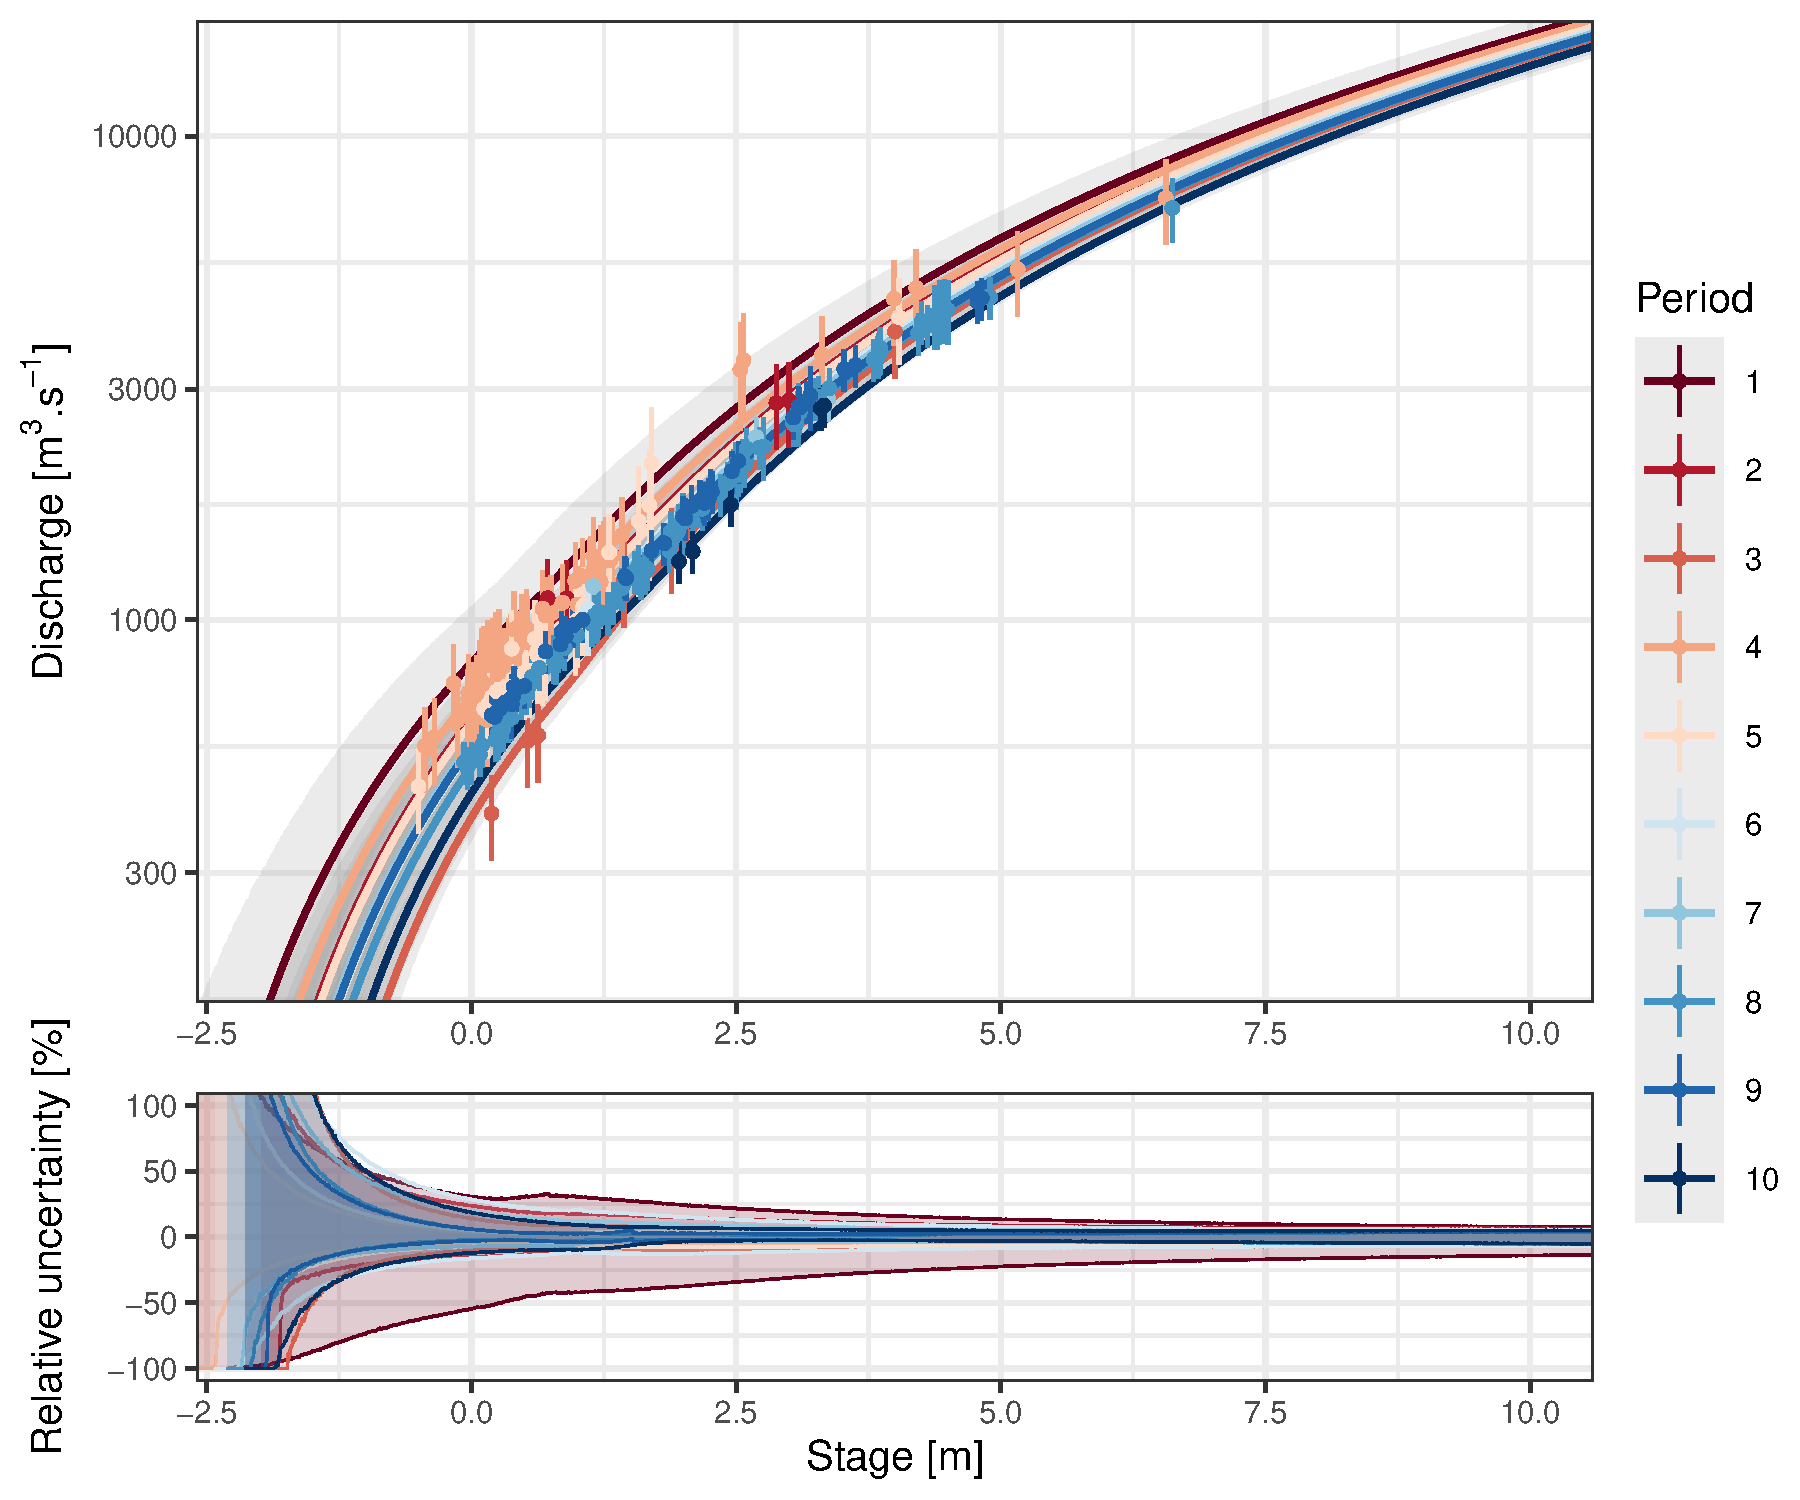
\includegraphics[width=\linewidth]{Figs/7a-RClog_ICdownPt.pdf}
            \caption{}
            \label{subfig:RcPt}
        \end{subfigure}
        \begin{subfigure}{0.49\textwidth}
            \centering
            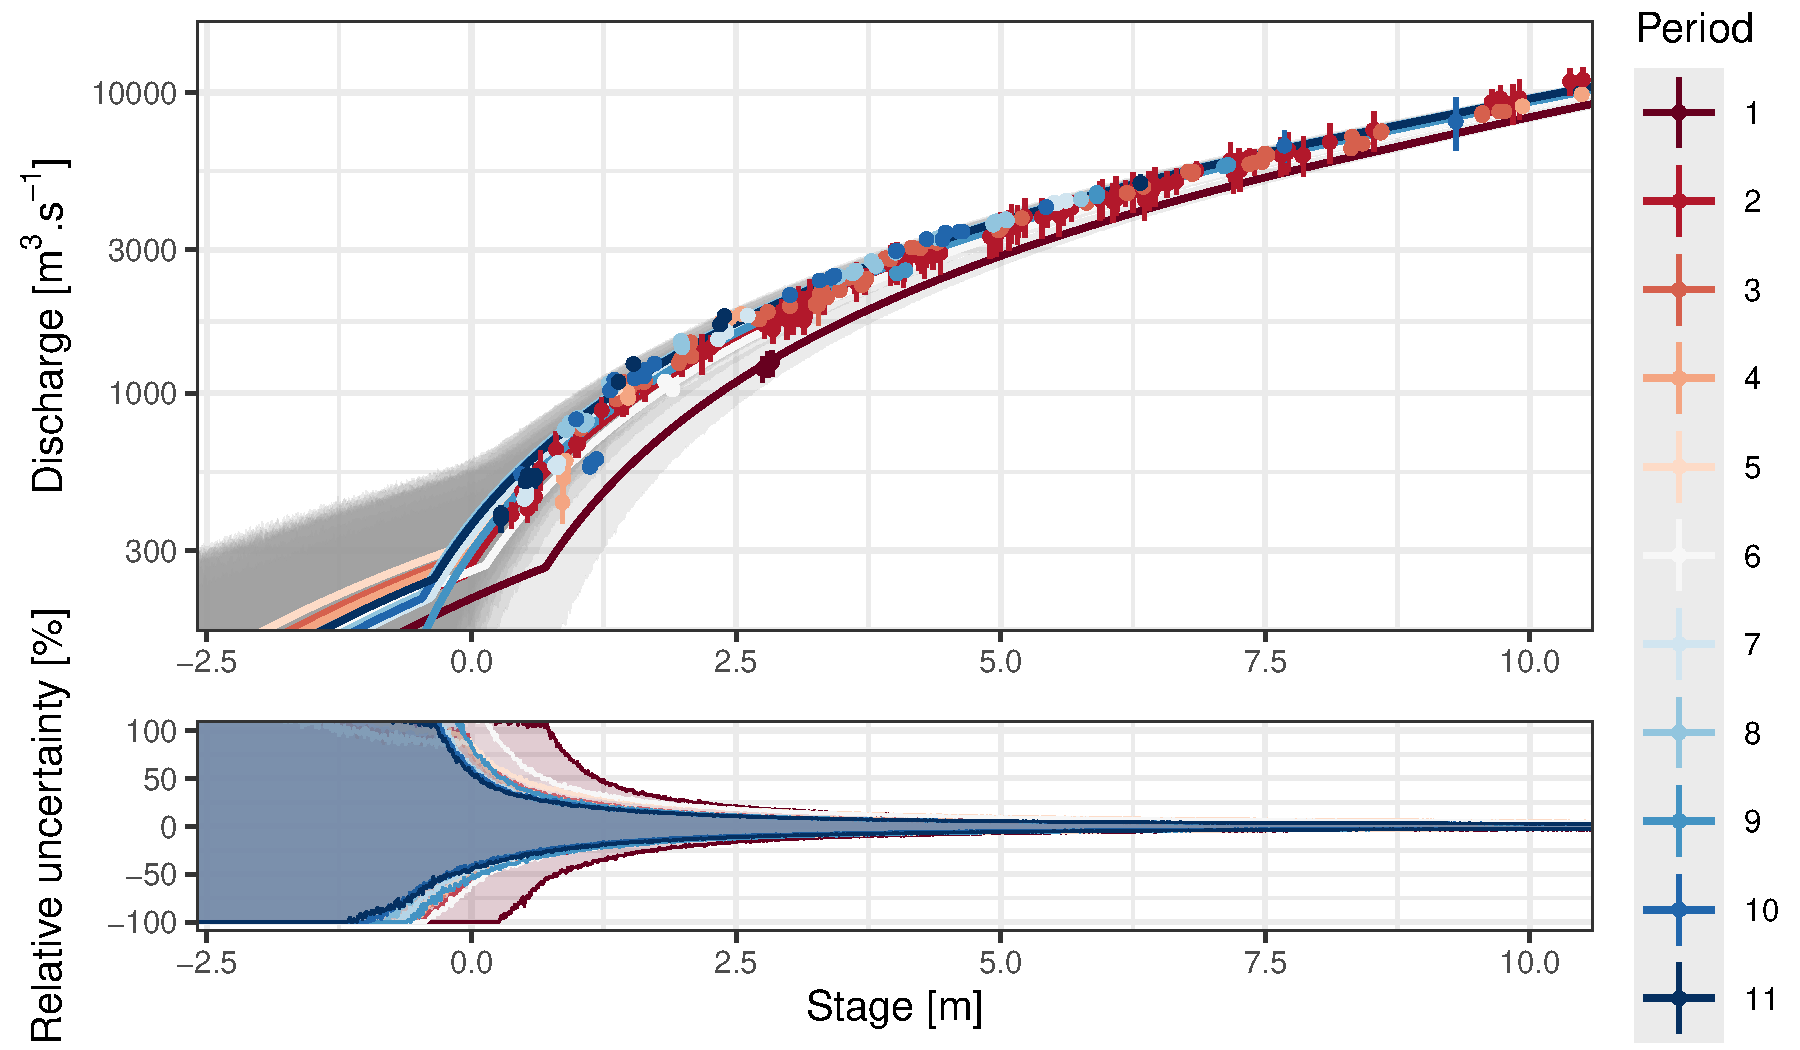
\includegraphics[width=\linewidth]{Figs/7b-RClog_ICdownRes.pdf}
            \caption{}
            \label{subfig:RcRes}
        \end{subfigure}
        
        \begin{subfigure}{0.49\textwidth}
            \centering
            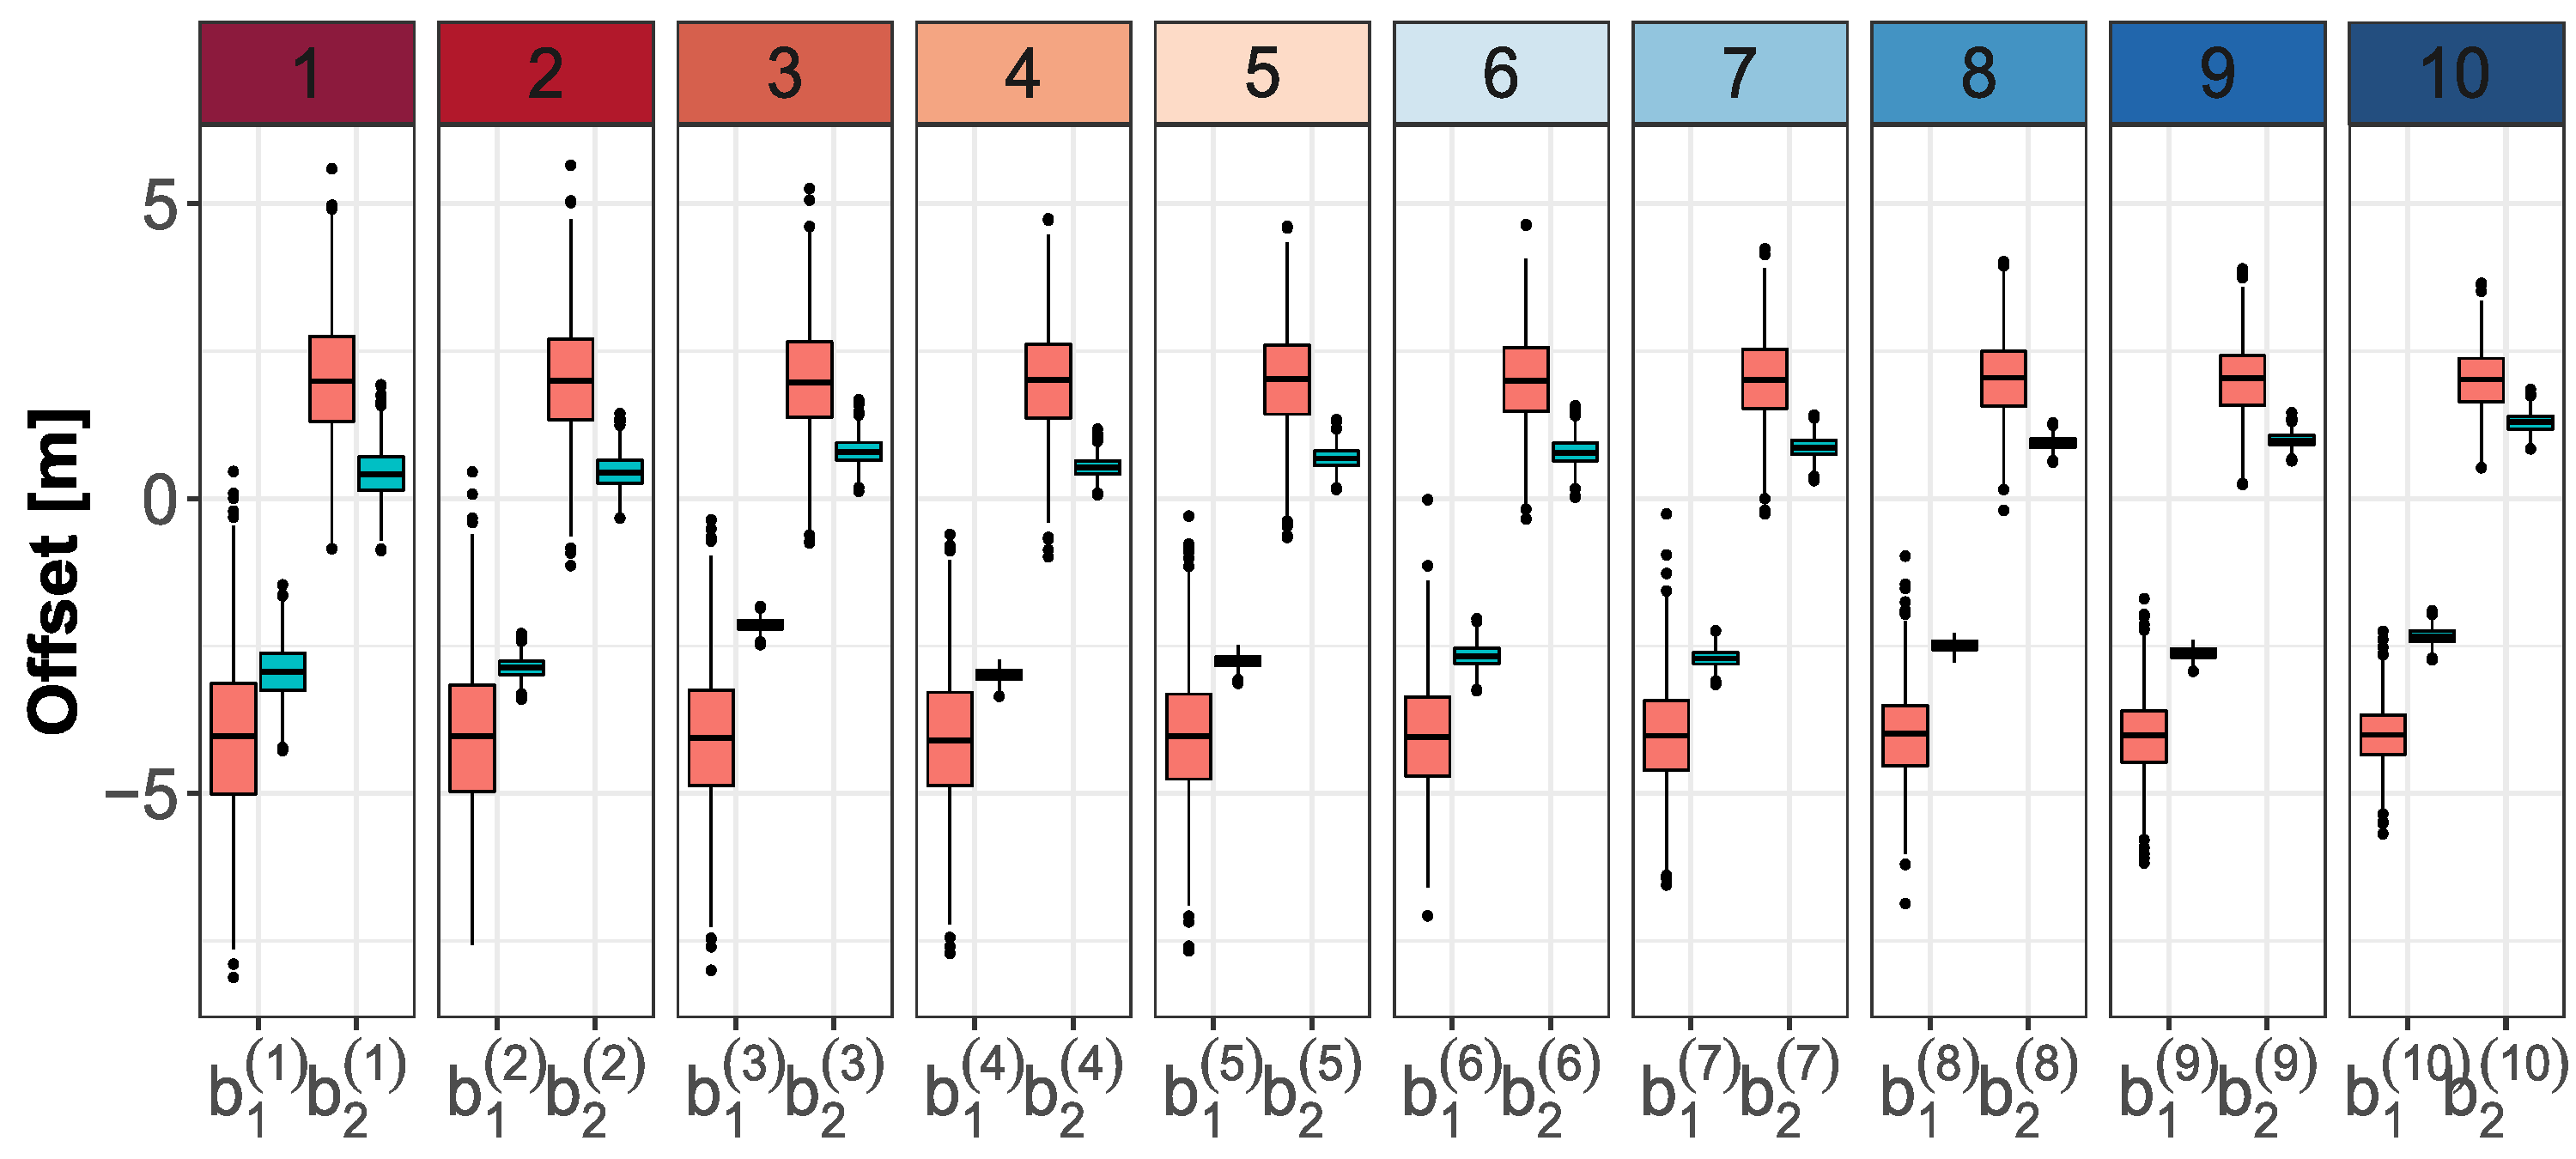
\includegraphics[width=\linewidth]{Figs/7c-bs_Pt.pdf}
            \caption{}
            \label{subfig:B'sPt}
        \end{subfigure}
        \begin{subfigure}{0.49\textwidth}
            \centering
            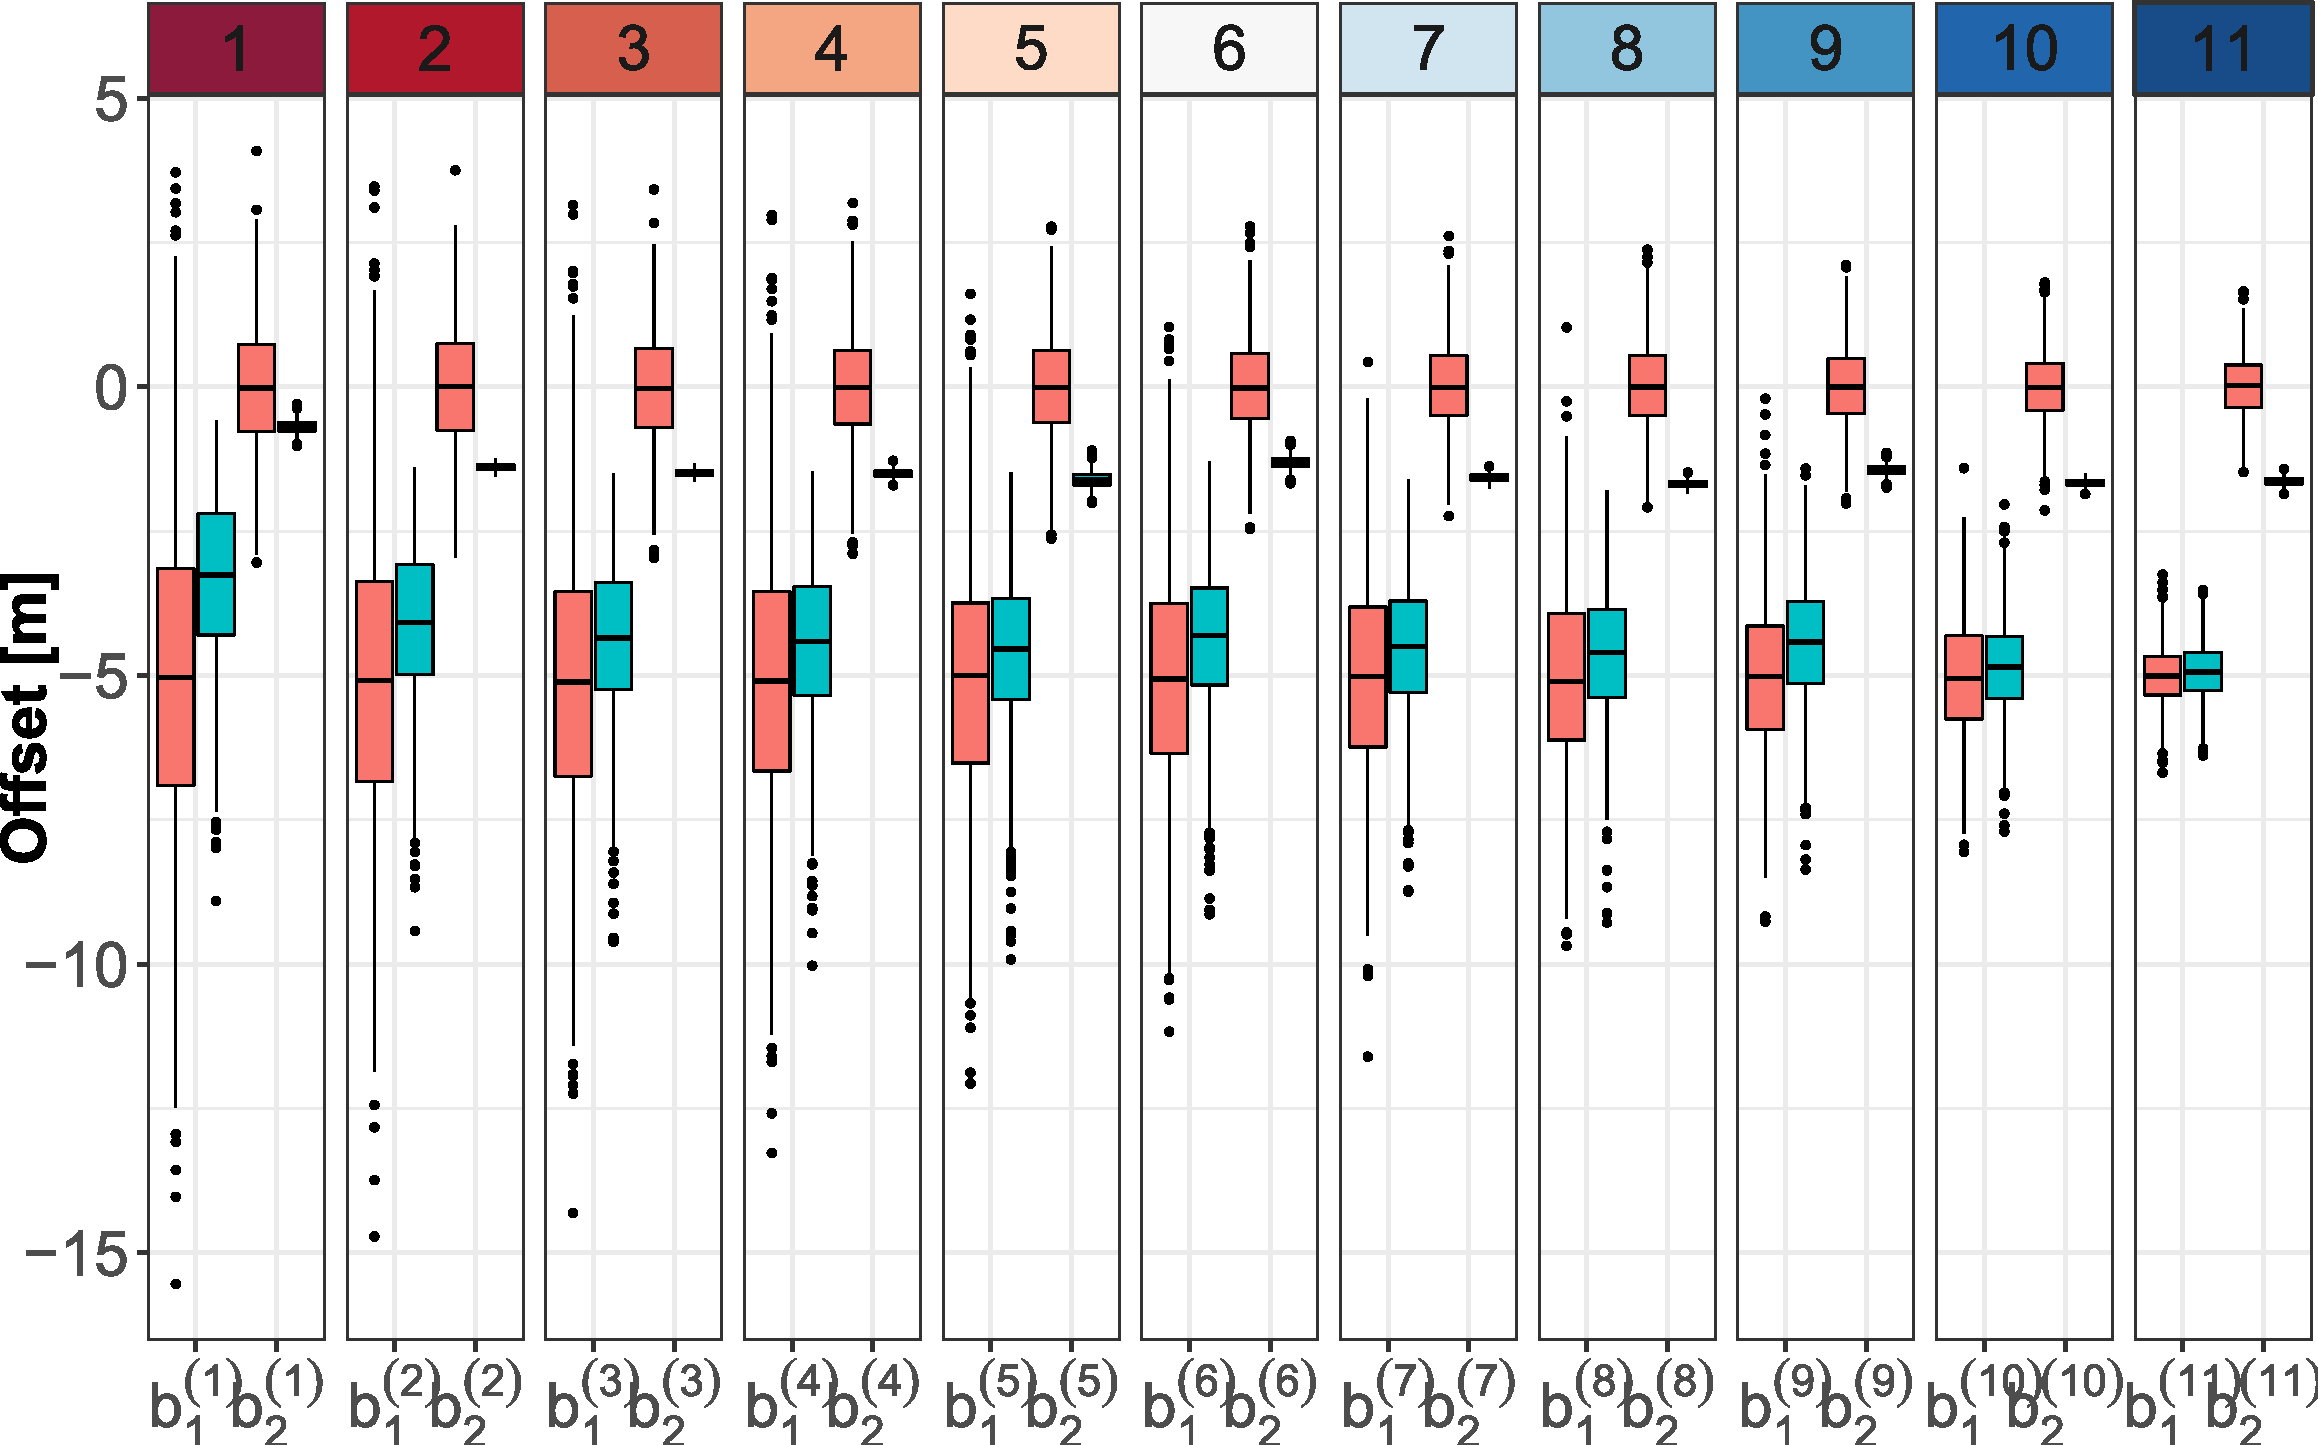
\includegraphics[width=\linewidth]{Figs/7d-bs_Restit.pdf}
            \caption{}
            \label{subfig:B'sRes}
        \end{subfigure}
        % \caption{Offsets priors and posteriors for Pont de Beaucaire (left) and Beaucaire restitution (right)}
        
        \begin{subfigure}{0.47\textwidth}
            \centering
            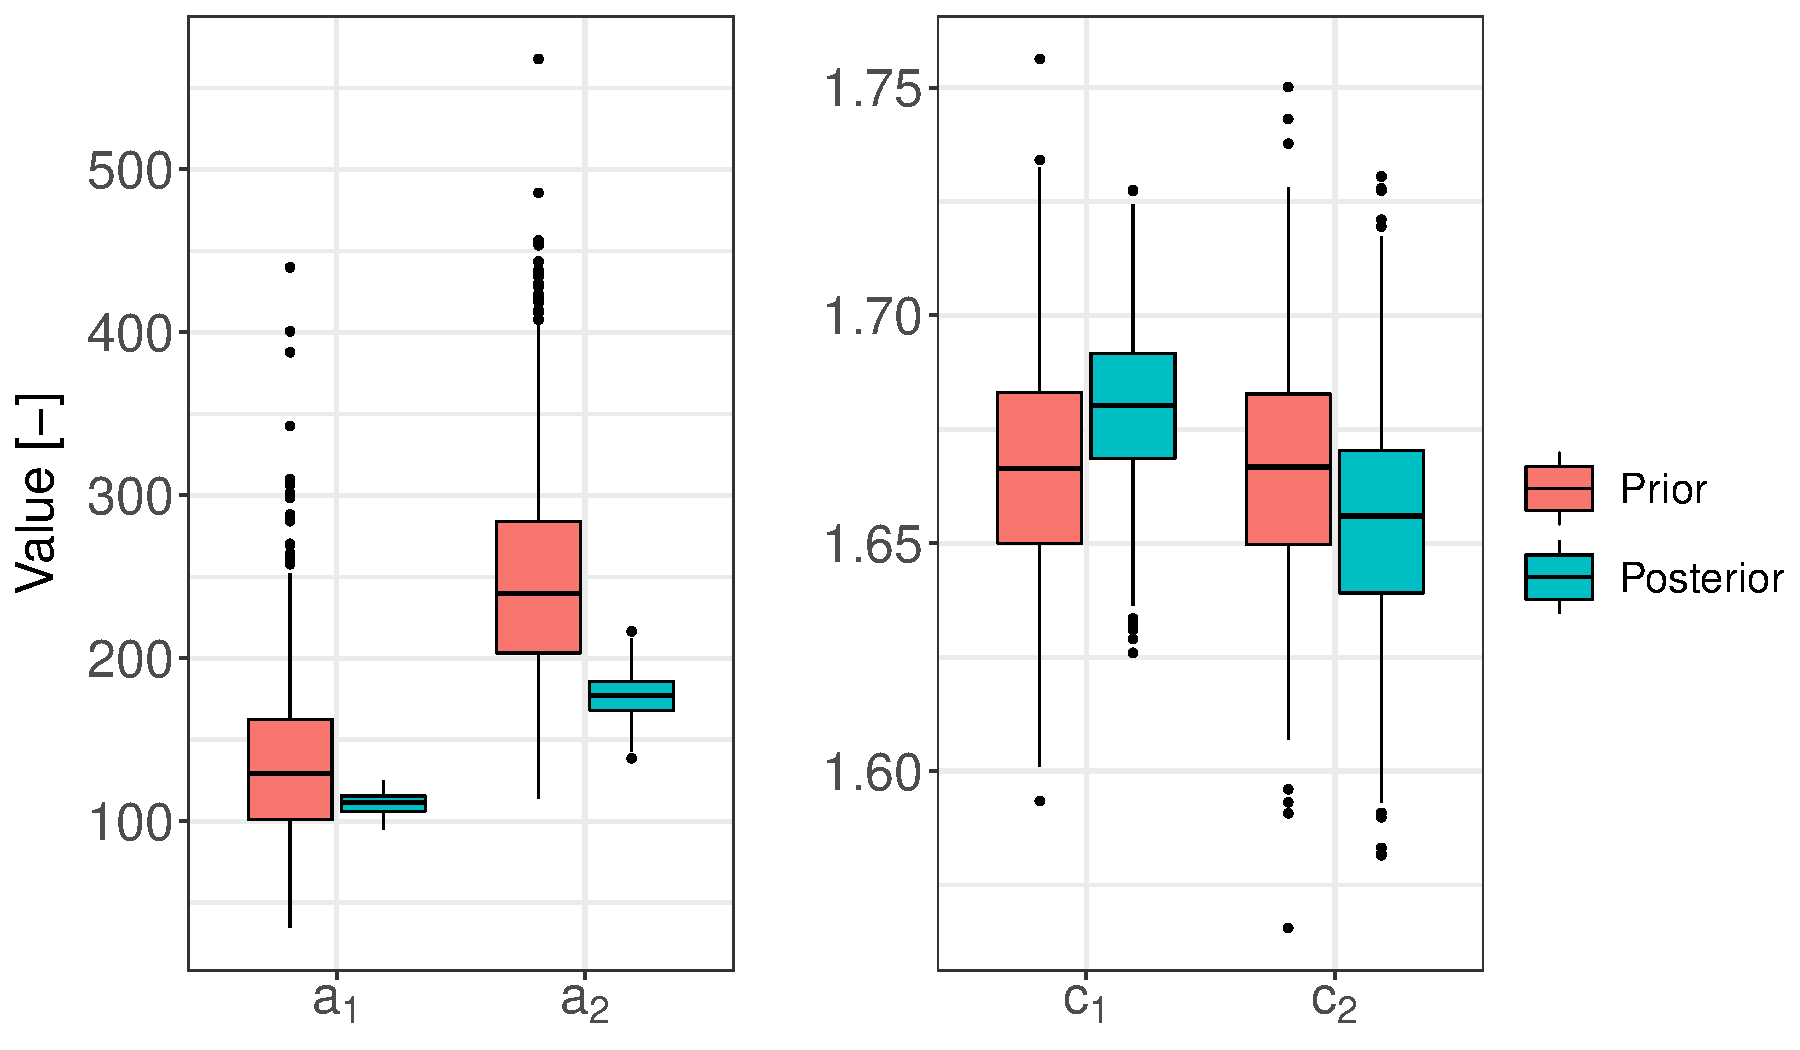
\includegraphics[width=\linewidth]{Figs/7e-a&csPt.pdf}
            \caption{}
            \label{subfig:a's and c's Pt}
        \end{subfigure}
        \begin{subfigure}{0.51\textwidth}
            \centering
            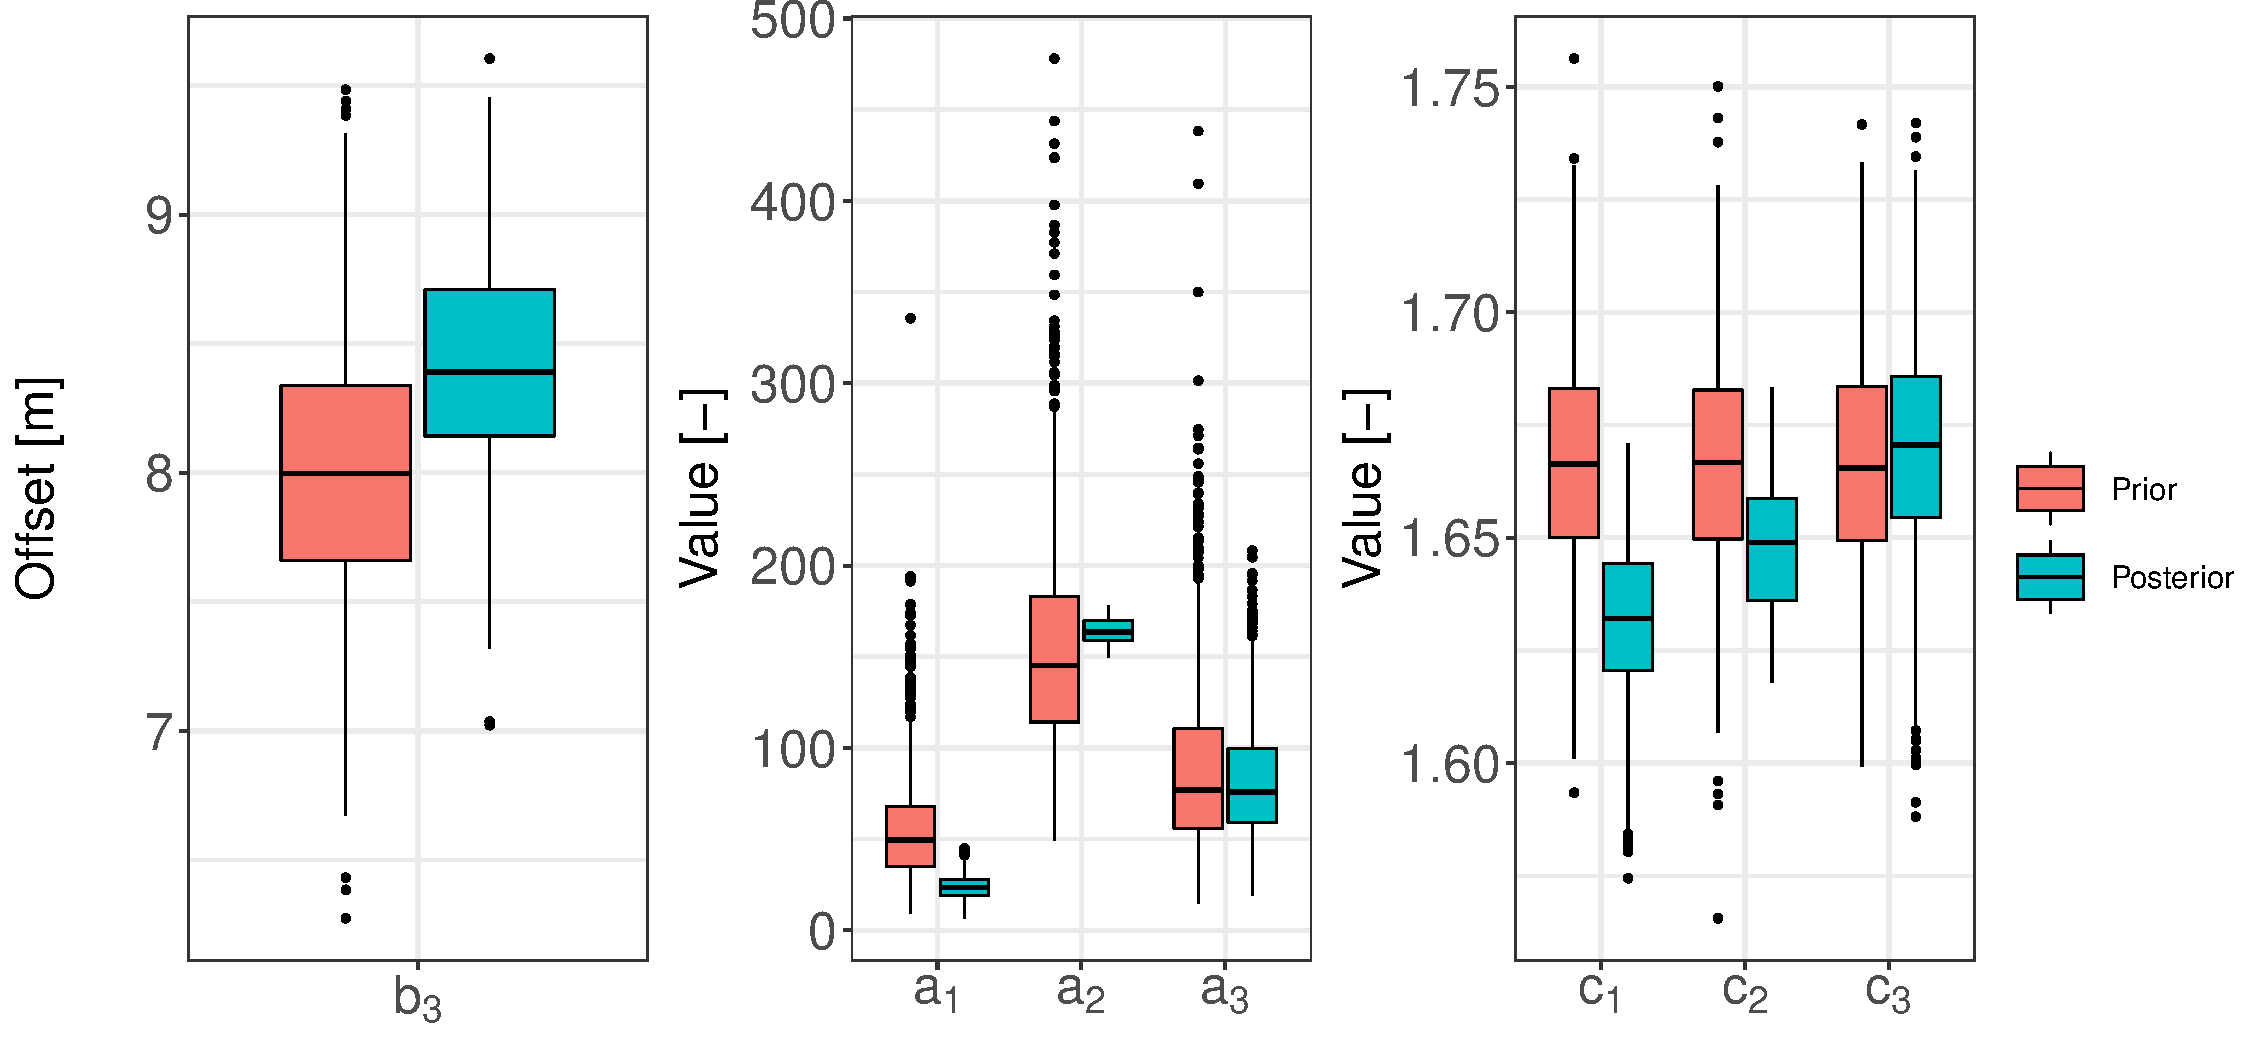
\includegraphics[width=\linewidth]{Figs/7f-b3_as_cs_Restit.pdf}
            \caption{}
            \label{subfig:bac'sRes}
        \end{subfigure}
        % \caption{Static parameters priors and posteriors for Pont de Beaucaire (left) and Beaucaire restitution (right)}
        \caption{Pont de Beaucaire (left) and Beaucaire Restitution (right) rating curves and relative 95\% uncertainty by respect to maxpost (first line), offsets priors and posteriors (second line) and static parameters priors and posteriors (third line). Rating curves are in logarithmic scale, solid lines represent maxpost values, grey transparent envelops represent 95\% uncertainty intervals and dots with error bars represent gaugings with 95\% uncertainty. Stable stage/discharge periods are numbered from the oldest to the latest.}
        \label{fig:RcsAndParams}
    \end{figure}
    
    \subsection{Stage errors}
    \label{sec:StageErrRes}
    
    The different error sources described in table \ref{tab:StageErr} are applied for both Beaucaire stations and propagated via Monte Carlo procedures. As seen in figure \ref{fig:StageErrAMAX}, measured stage is below stage uncertainty interval before 1840 at Pont de Beaucaire. This is due to the exponential distribution used to model measurement frequency error which is predominant here and has, by definition, only positive results. The upper uncertainty bound is sometimes 1.5 meters higher than the measured stage, highlighting the importance of considering this type of error. Apart from that, the uncertainty of AMAX stages is decreasing over time as the measurement frequency and precision are improving. The width of the 95\% uncertainty interval is equal to 1.7m before 1840, 0.3m between 1840 and 1967, and 0.24m at Beaucaire Restitution (1970-2020). The 5m threshold above which hourly measurements were done after 1840 is explaining an important reduction of the uncertainty. After this date, the uncertainty is controlled by the exceedance of this 5m threshold, the AMAX below 5m being penalized by measurement frequency error $\delta_5$ that is considered negligible for hourly measurements made above 5m. Beaucaire Restitution uncertainty is smaller than Pont de Beaucaire uncertainty. The difference between uncertainty bounds and originally measured stages is presented in the bottom part of figure \ref{fig:StageErrAMAX}. The median of stage realisations is showing some fluctuations that are mainly due to datum reference errors that are drawn every 25 years at Pont de Beaucaire.
    
    \begin{figure}[h!]
        \centering
        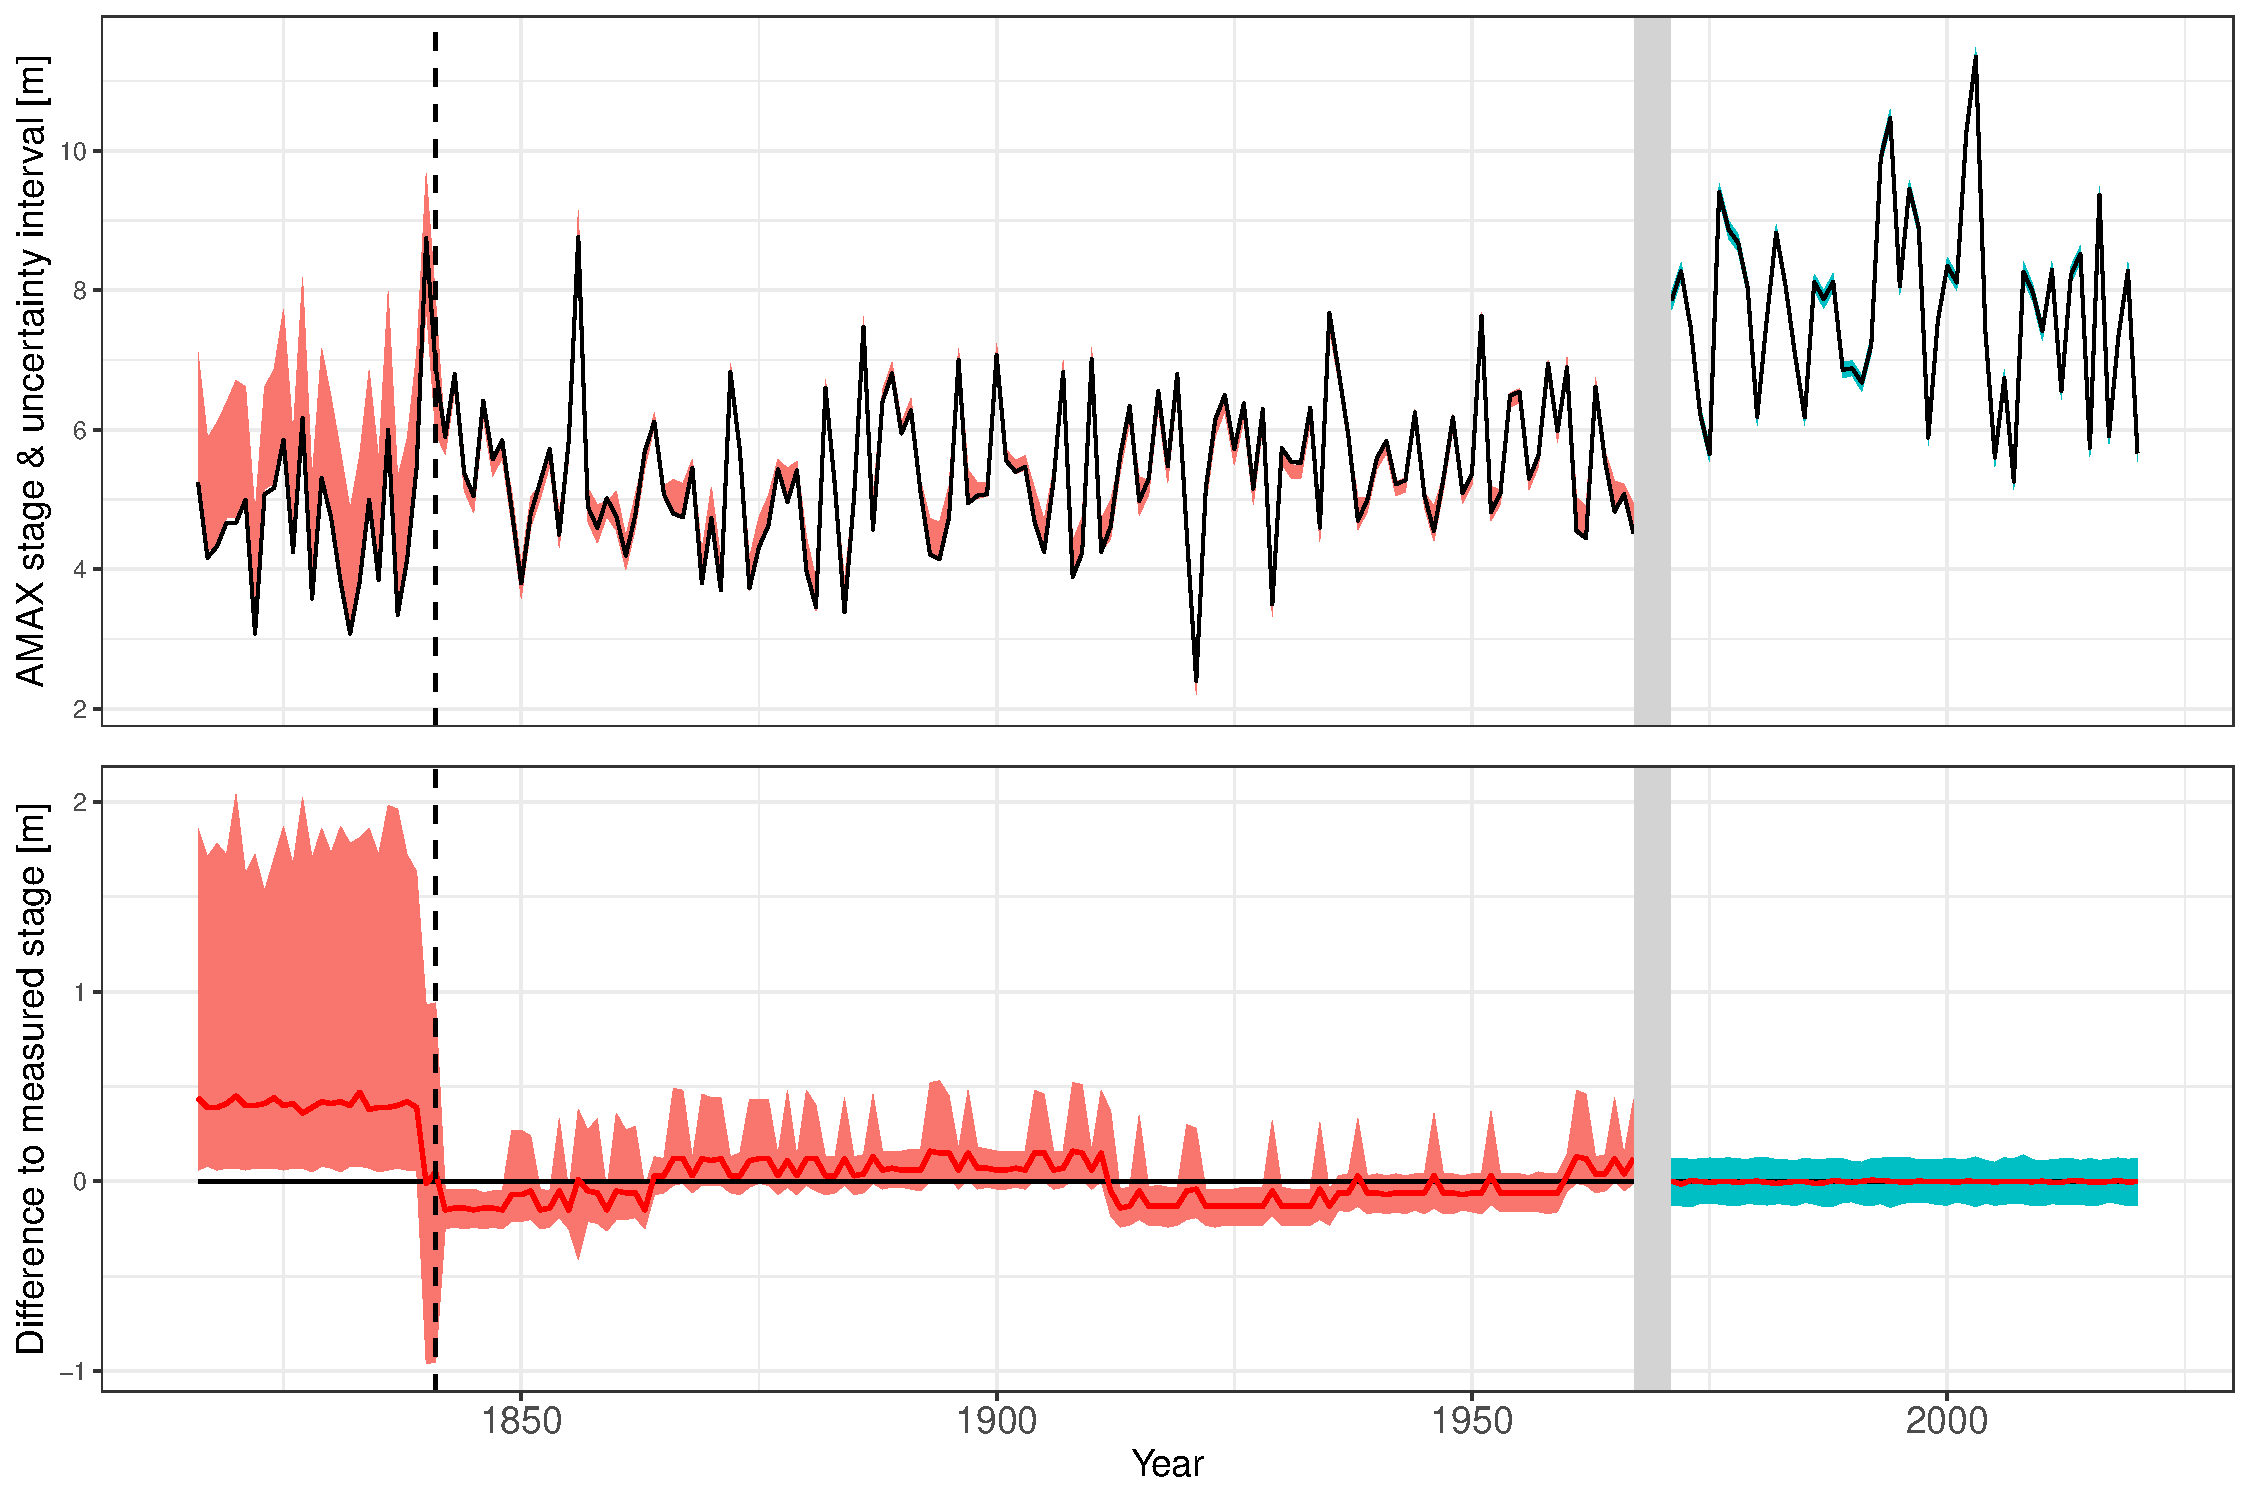
\includegraphics[width=0.8\linewidth]{Figs/8-StageErrorAMAX_BOTH.pdf}\hfill
        \caption{Top : AMAX stage uncertainty at Pont de Beaucaire (red) and Beaucaire Restitution (blue). Solid line represents measured stage. Red and blue ribbons respectively represents the 95\% uncertainty interval at Pont de Beaucaire and Beaucaire Restitution.
        Bottom : Difference between stage uncertainty bounds and originally measured stage for both stations (red and blue ribbons). Solid red lines represents the median of stage realisations and the horizontal black line at 0m stands for the measured AMAX stages. The vertical dotted line stands for the year 1840 from which hourly measurement were done above a 5m threshold. Grey band represents the years of Vallabrègues hydraulic works.}
        \label{fig:StageErrAMAX}
    \end{figure}
  

    \subsection{Total streamflow uncertainties}
    
    Stage uncertainties were propagated through uncertain rating curves, allowing to access to the contribution of each source that are represented in three categories: parametric and remnant uncertainties (from rating curves), and stage uncertainties. The maxpost AMAX series is obtained by propagating the the median of stage realisations through maxpost rating curves. The result is presented in Figure \ref{fig:ICtot_both} for both Beaucaire gauges, allowing a visualisation of streamflow uncertainties from 1816 to 2020. Streamflow uncertainty, although fluctuating, appears to decrease over time. From +/- 30\% before 1840, and +/- 10\% before 1967, to +/- 5\% at Beaucaire Restitution (1967-2020). Stage uncertainty appears predominant at Pont de Beaucaire, as well as rating curve parametric uncertainty, originating from the difficulty to estimate rating curve parameters with only few gaugings. Thus, parametric uncertainty is reduced for properly gauged periods. During the Vallabrègues hydraulic system construction (1967 - 1970), the discharges of the Durance River, one of the major tributaries, were deviated from the Rhône River course. AMAX discharges of these missing years were reconstructed by CNR with upstream gauging stations. The uncertainty around these reconstructed discharges is assumed Gaussian distribution with mean being the reconstructed values and standard deviation being 10\% of those values (represented in grey).
    
    \begin{figure}[h!]
        \centering
        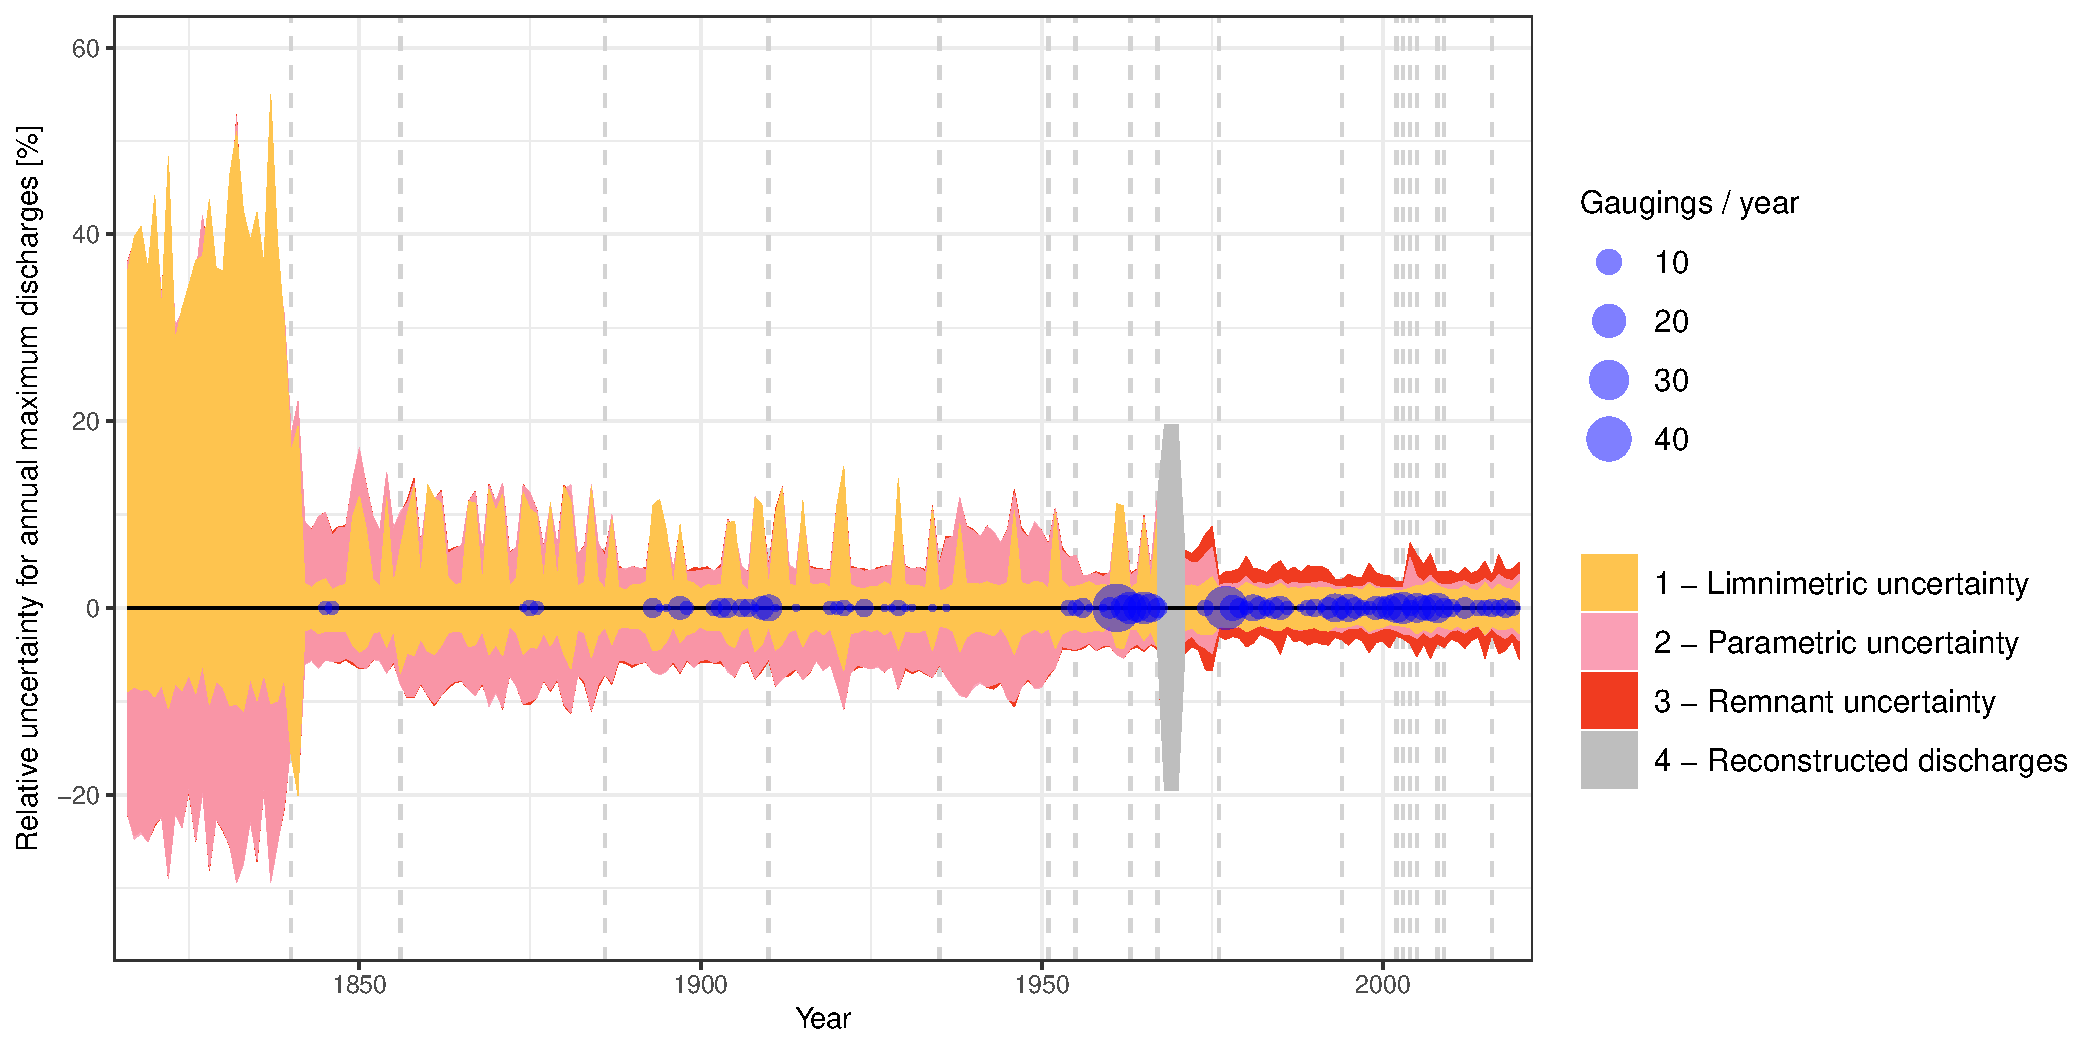
\includegraphics[width=\textwidth]{Figs/9-IC_AMAX_Both.pdf}
        \caption{AMAX maxpost discharges (black solid line) and uncertainty bounds for the three sources of streamflow uncertainties at Beaucaire (1816 - 2020). Vertical dotted lines represent rating shifts and blue dots area is proportional to the number of gaugings by year.}
        \label{fig:ICtot_both}
    \end{figure}
    
   
    \subsection{Flood frequency analysis}
    
        \subsubsection{Streamflow series homogeneity}
           
        \paragraph{}
        Streamflow series homogeneity is an essential prerequisite to FFA as the latter is based on the hypothesis of iid random variables. In order to check this hypothesis, the Mann-Kendall non-parametric test (\citet{mann_nonparametric_1945}, \citet{kendall_rank_1948}) is applied to AMAX series at Beaucaire. As streamflow uncertainty is carried by $n$ AMAX discharge realisations, the homogeneity test is applied on each of the $n$ AMAX series. 83\% of the Mann-Kendall tests concluded in the non-rejection of the null hypothesis (there is no trend in the series) with a 0.05 significance level. We assume that this is enough to consider this series homogeneous and to proceed to FFA. 
        
        \subsubsection{Flood frequency analysis}
        
       The GEV distribution estimation procedure described in section \ref{sec:STOODS} is applied to the 205 years long AMAX discharges series at Beaucaire accounting for uncertainties. Vague priors are given to GEV parameters : flat priors for location and scale parameters, and Gaussian with zero mean and 0.2 standard deviation for the shape parameter.
       Flood quantiles results (figure \ref{fig:GEV205y}) show that streamflow uncertainty dominates for the lowest return periods, but sampling uncertainty is taking over when the return period tends toward 1000 years (see \ref{subfig:UKplot4cases} bottom right figure for a better understanding of the respective part of each source of uncertainty in this 205 years case). The AMAX observed discharges display a large variability of streamflow uncertainties. The three largest floods of this 205 years sample (1840, 1856 and 2003, by chronological order and from the most precise to the most uncertain) are illustrating this point. Thus, not considering 1840 and 1856 years could have a large effect on the estimation of the maxpost quantiles value, as well as the uncertainty bounds values. This is explored next by varying the sample size.
       
       \begin{figure}[h!]
            \centering
            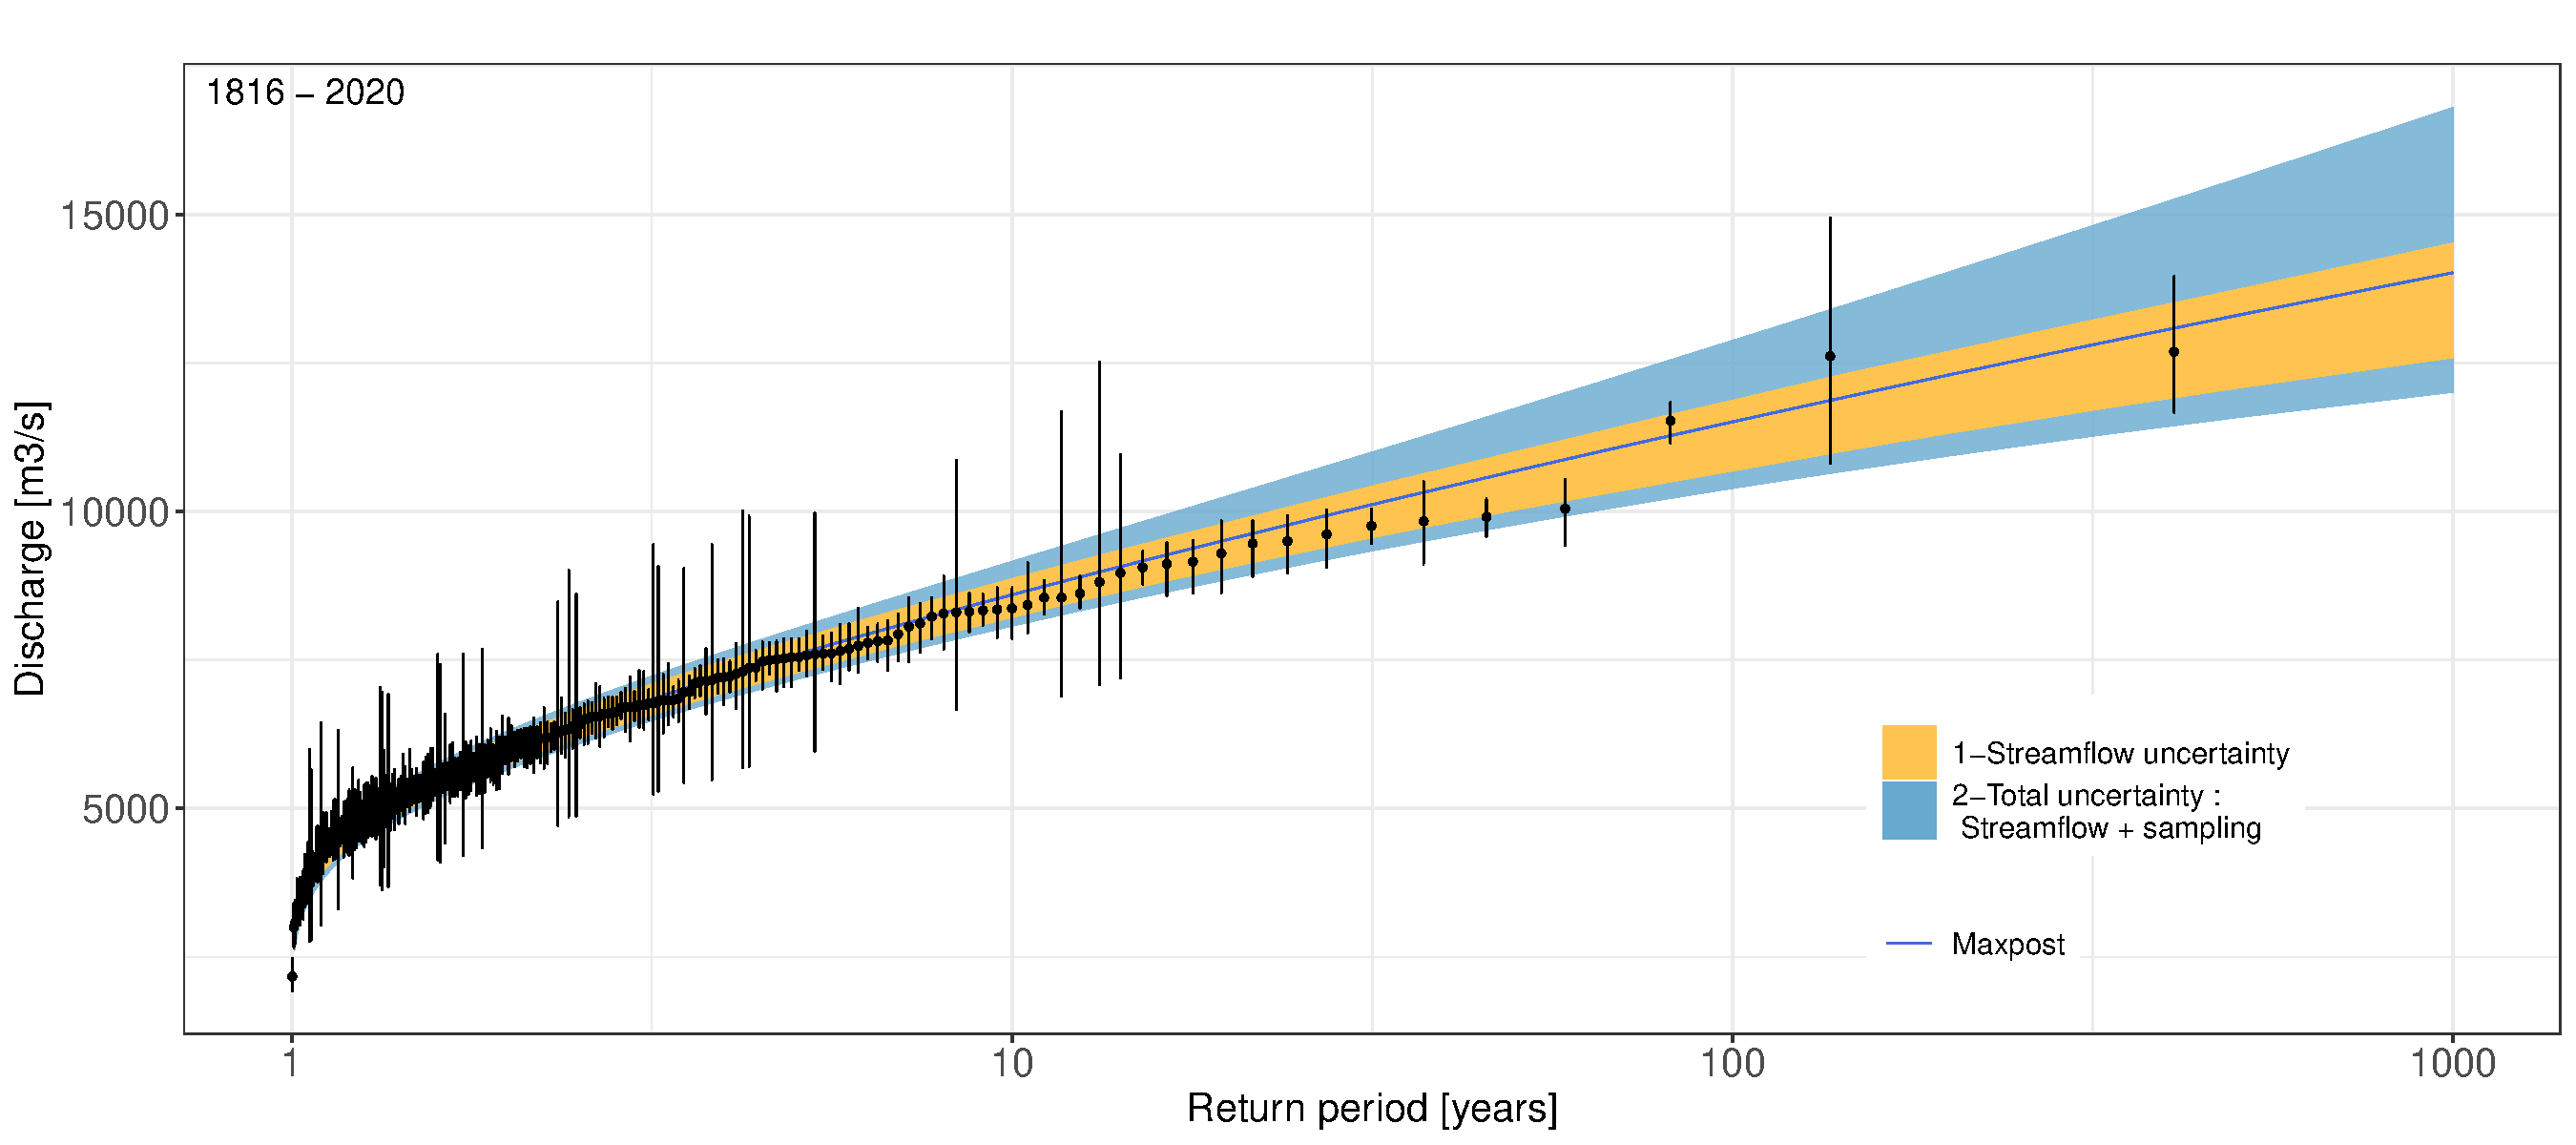
\includegraphics[width=0.7\linewidth]{Figs/10-GeV_205years.pdf}
            \caption{Flood quantiles 95\% uncertainty interval for both streamflow and total (streamflow + sampling) uncertainties. Error bars represent the AMAX observed discharges with 95\% streamflow uncertainty.}
            \label{fig:GEV205y}
        \end{figure}            
        
        \begin{figure}[h!]
            \centering
            \begin{subfigure}{0.49\linewidth}
                \centering
                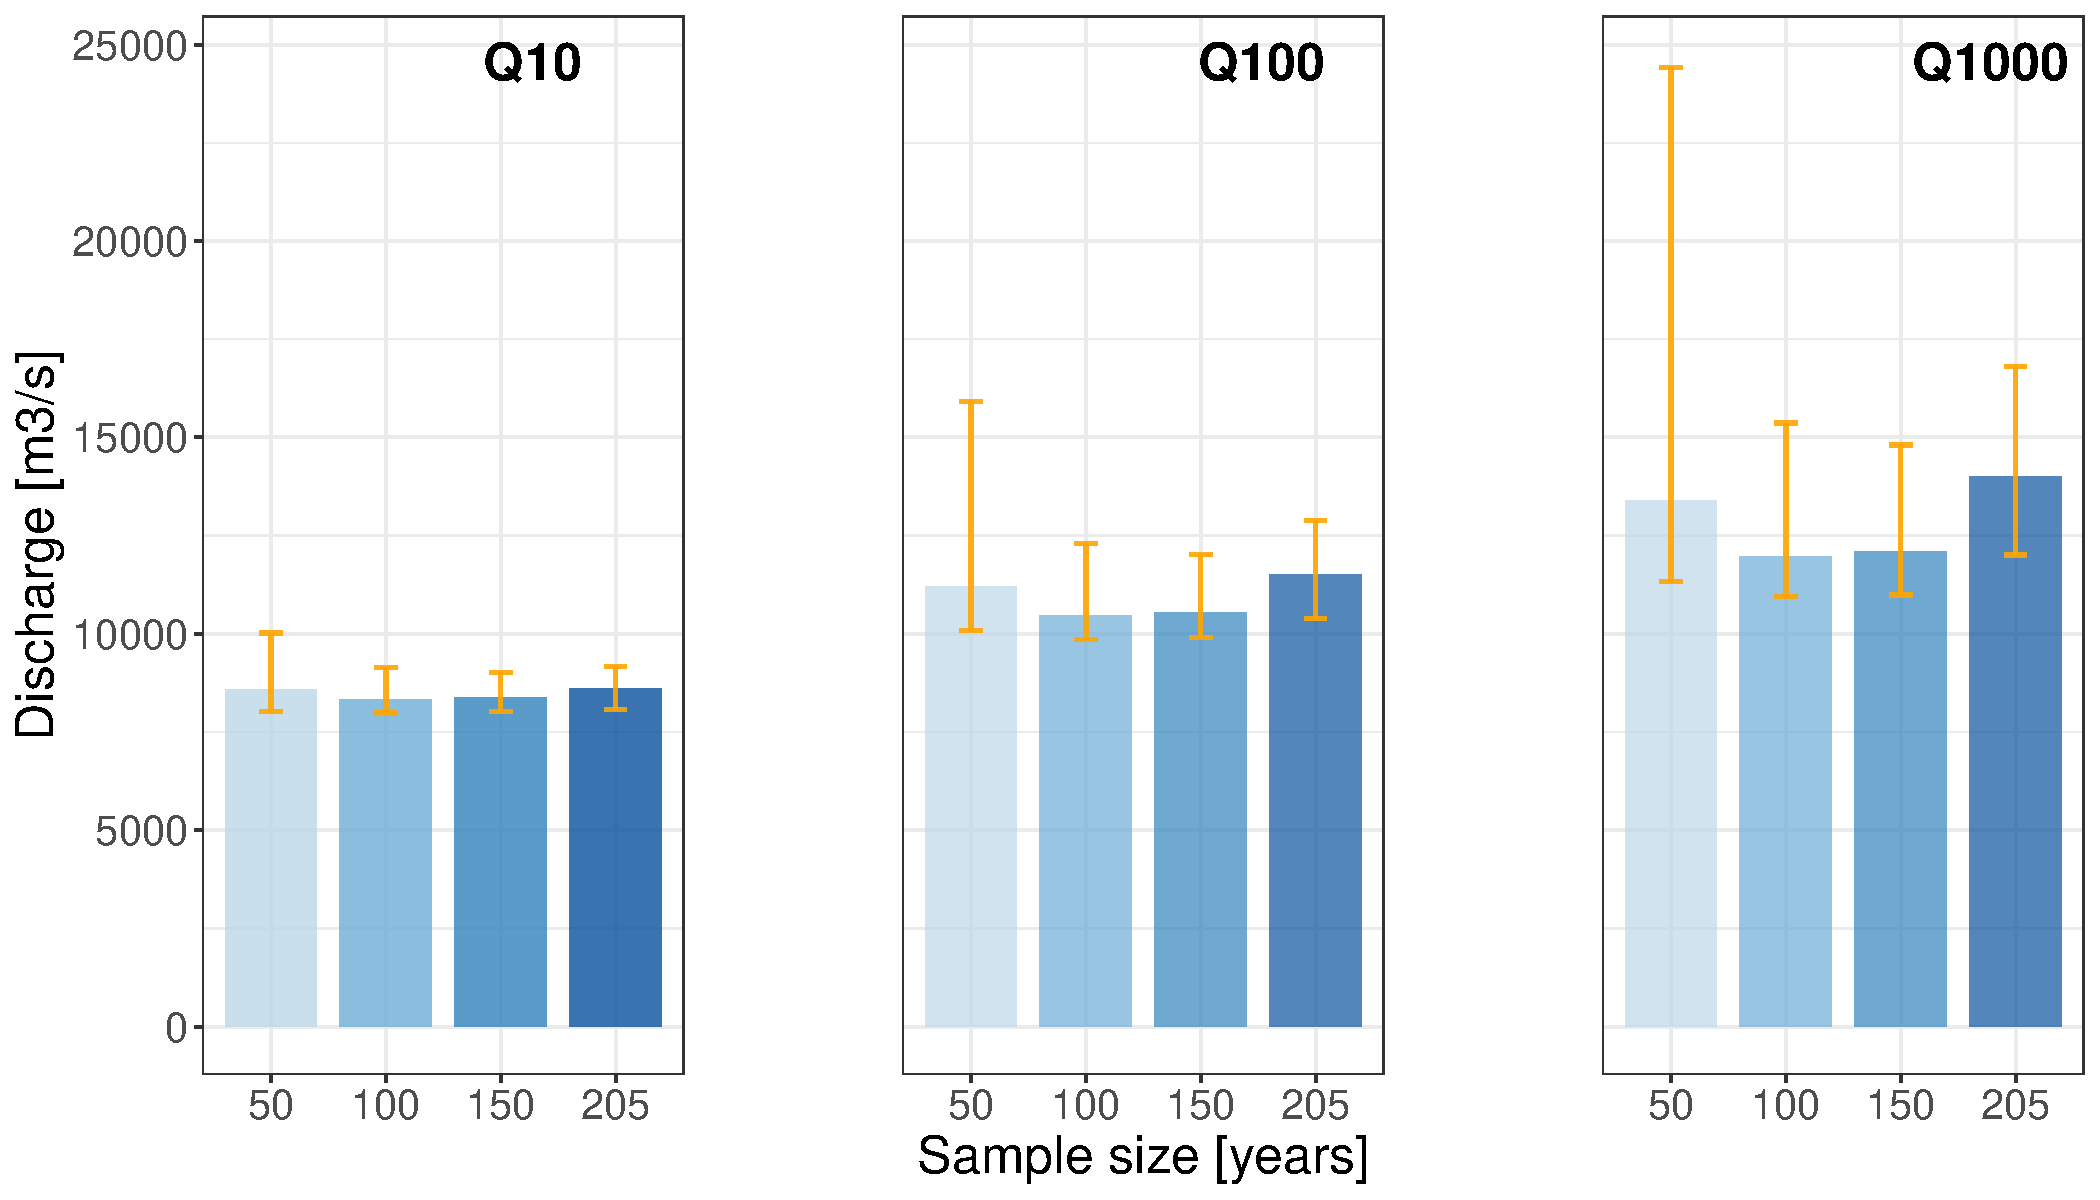
\includegraphics[width=1\linewidth]{Figs/11a-BarplotQuantiles4cases.pdf}
                \caption{}
                \label{subfig:Form4cases}
            \end{subfigure}
            \begin{subfigure}{.49\textwidth}
                \centering  
                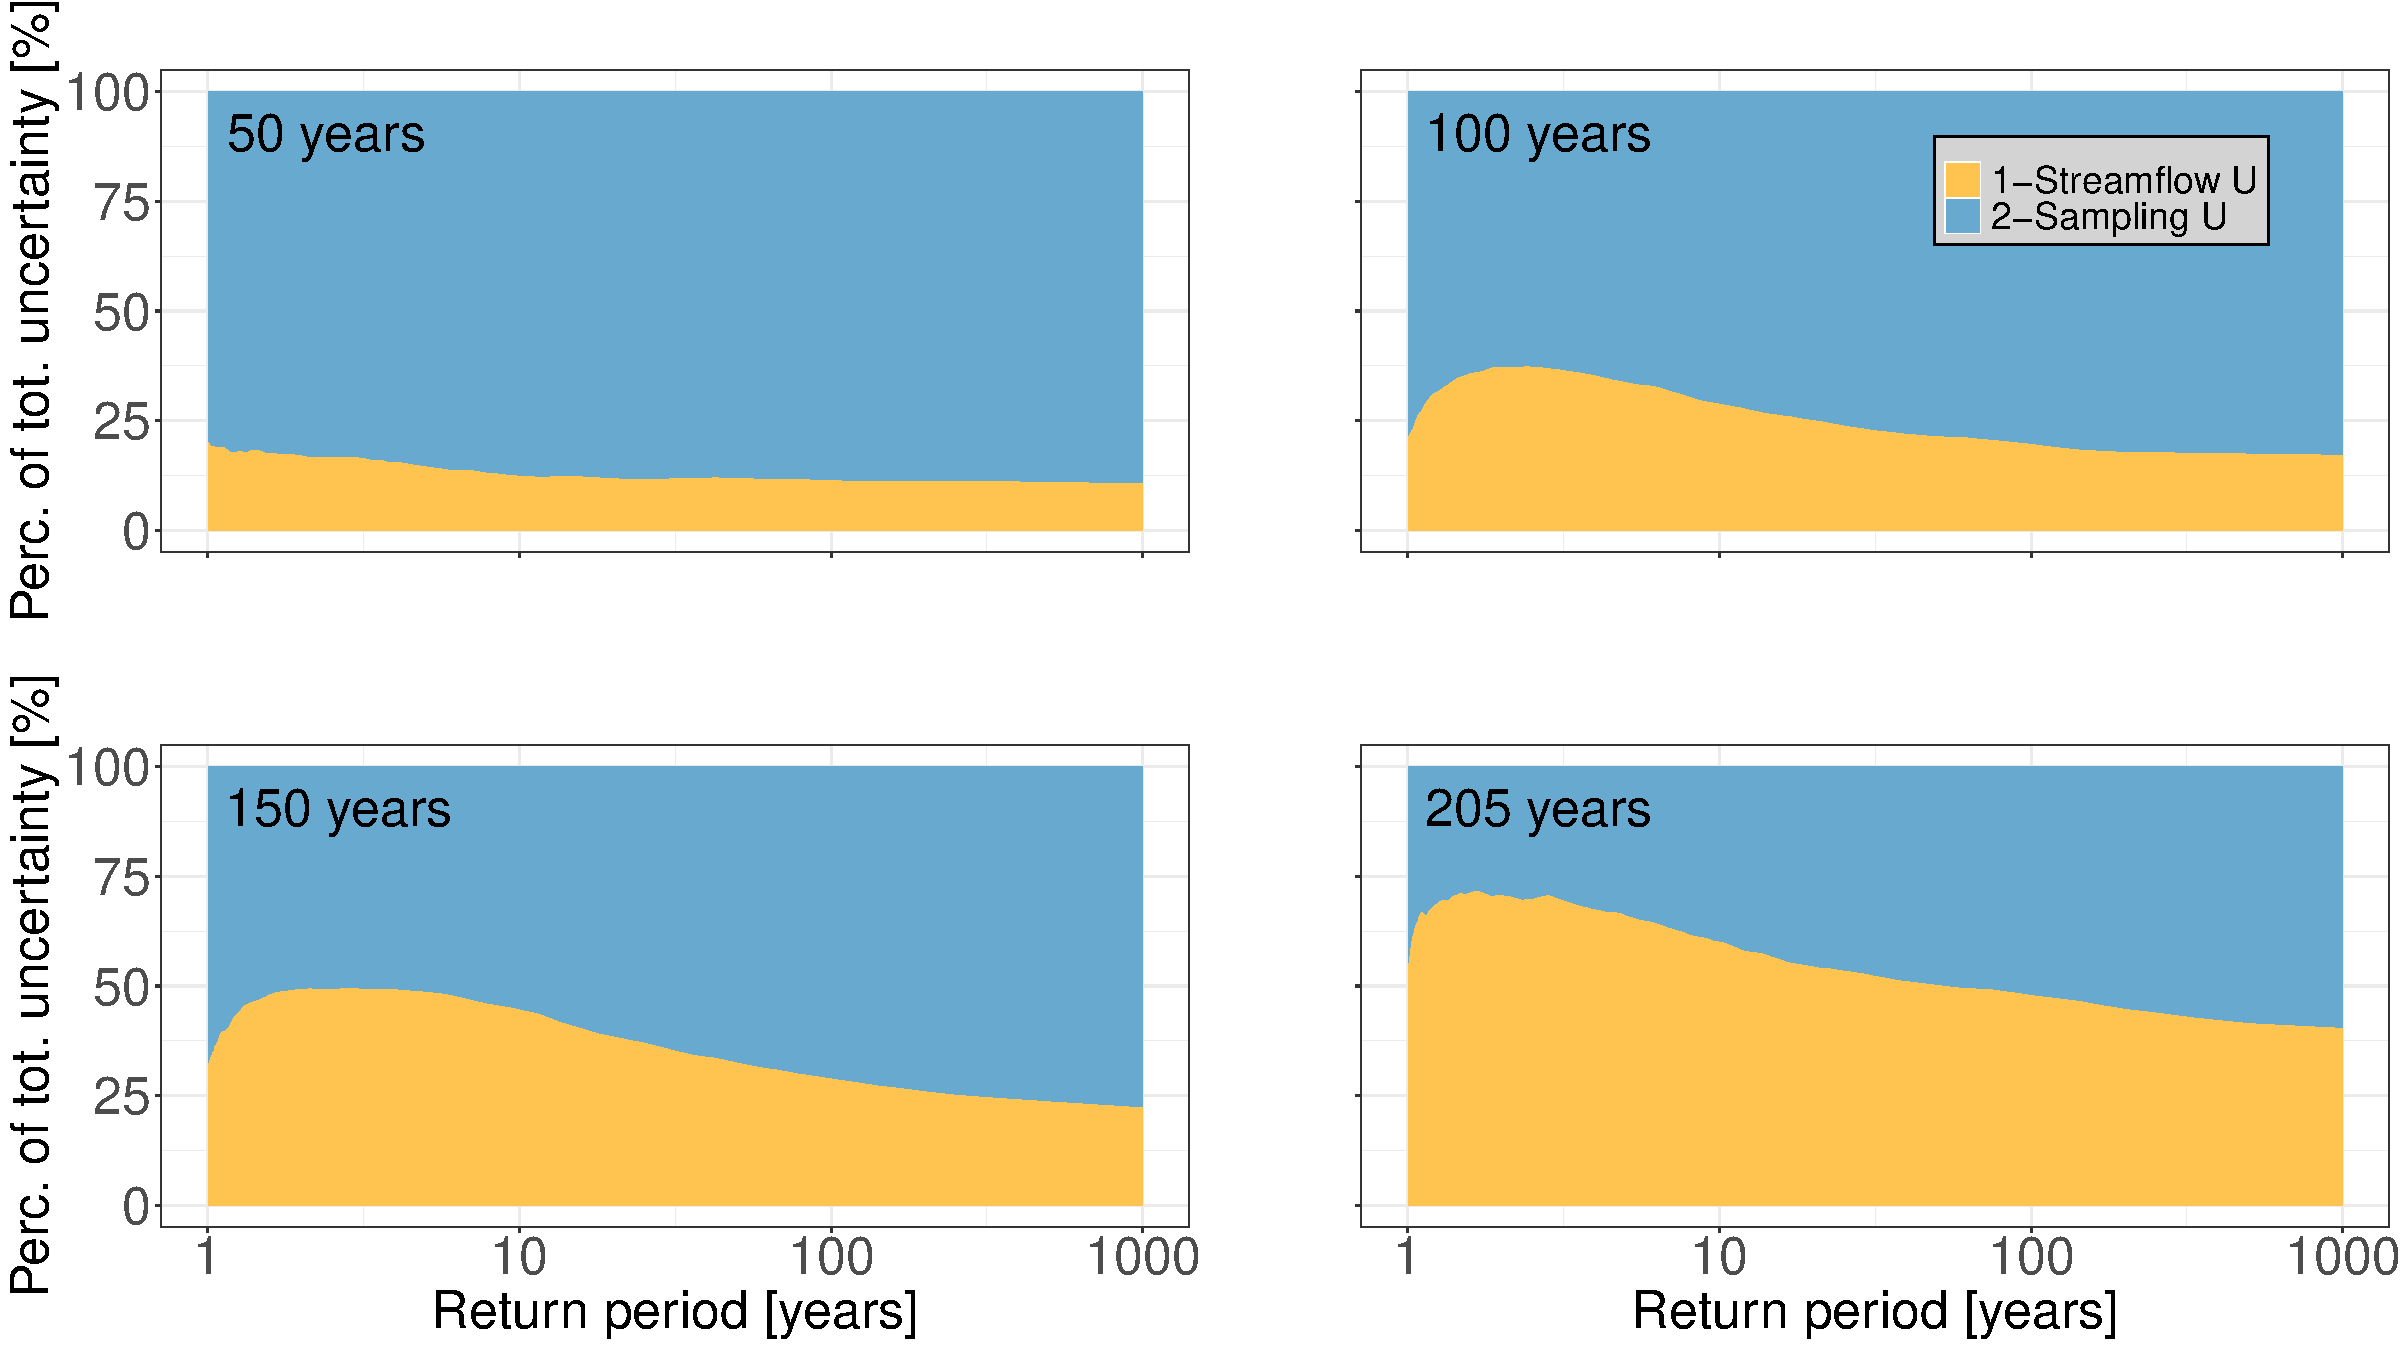
\includegraphics[width=\linewidth]{Figs/11b-Ukplot4cases.pdf}
                \caption{}
                \label{subfig:BarplotQuantilesGev}
            \end{subfigure}
            
            \begin{subfigure}{0.49\textwidth}
                \centering
                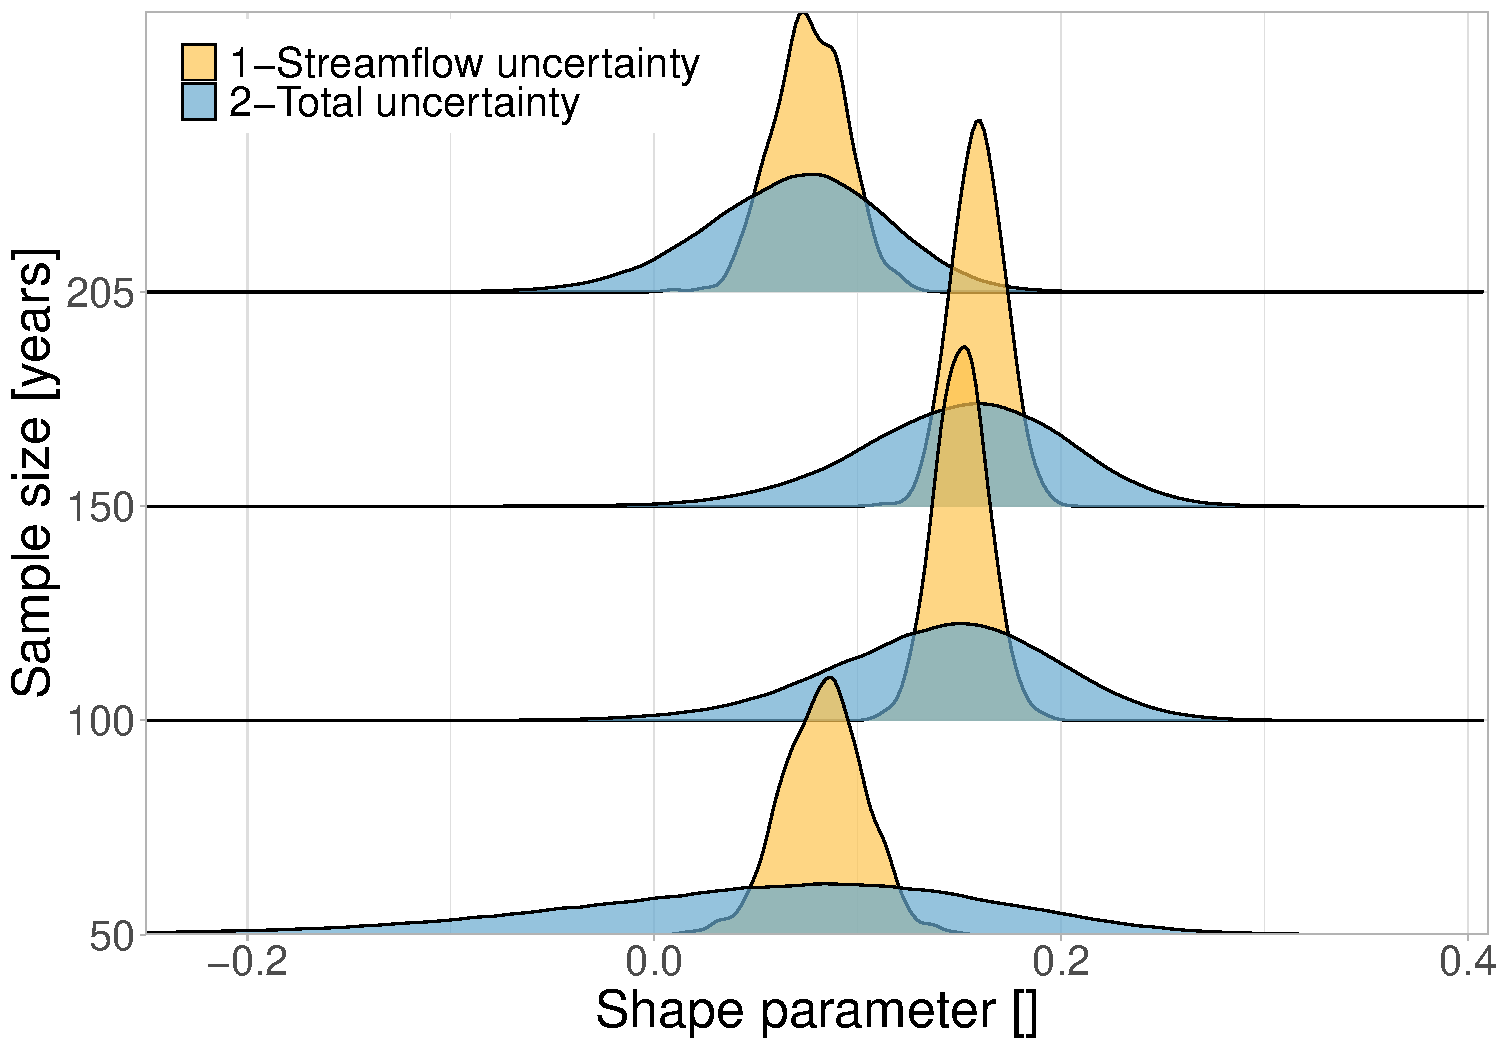
\includegraphics[width=\linewidth]{Figs/11c-Shape_4cases.pdf}
                \caption{}
                \label{subfig:UKplot4cases}
            \end{subfigure}
            \begin{subfigure}{0.49\textwidth}
                \centering
                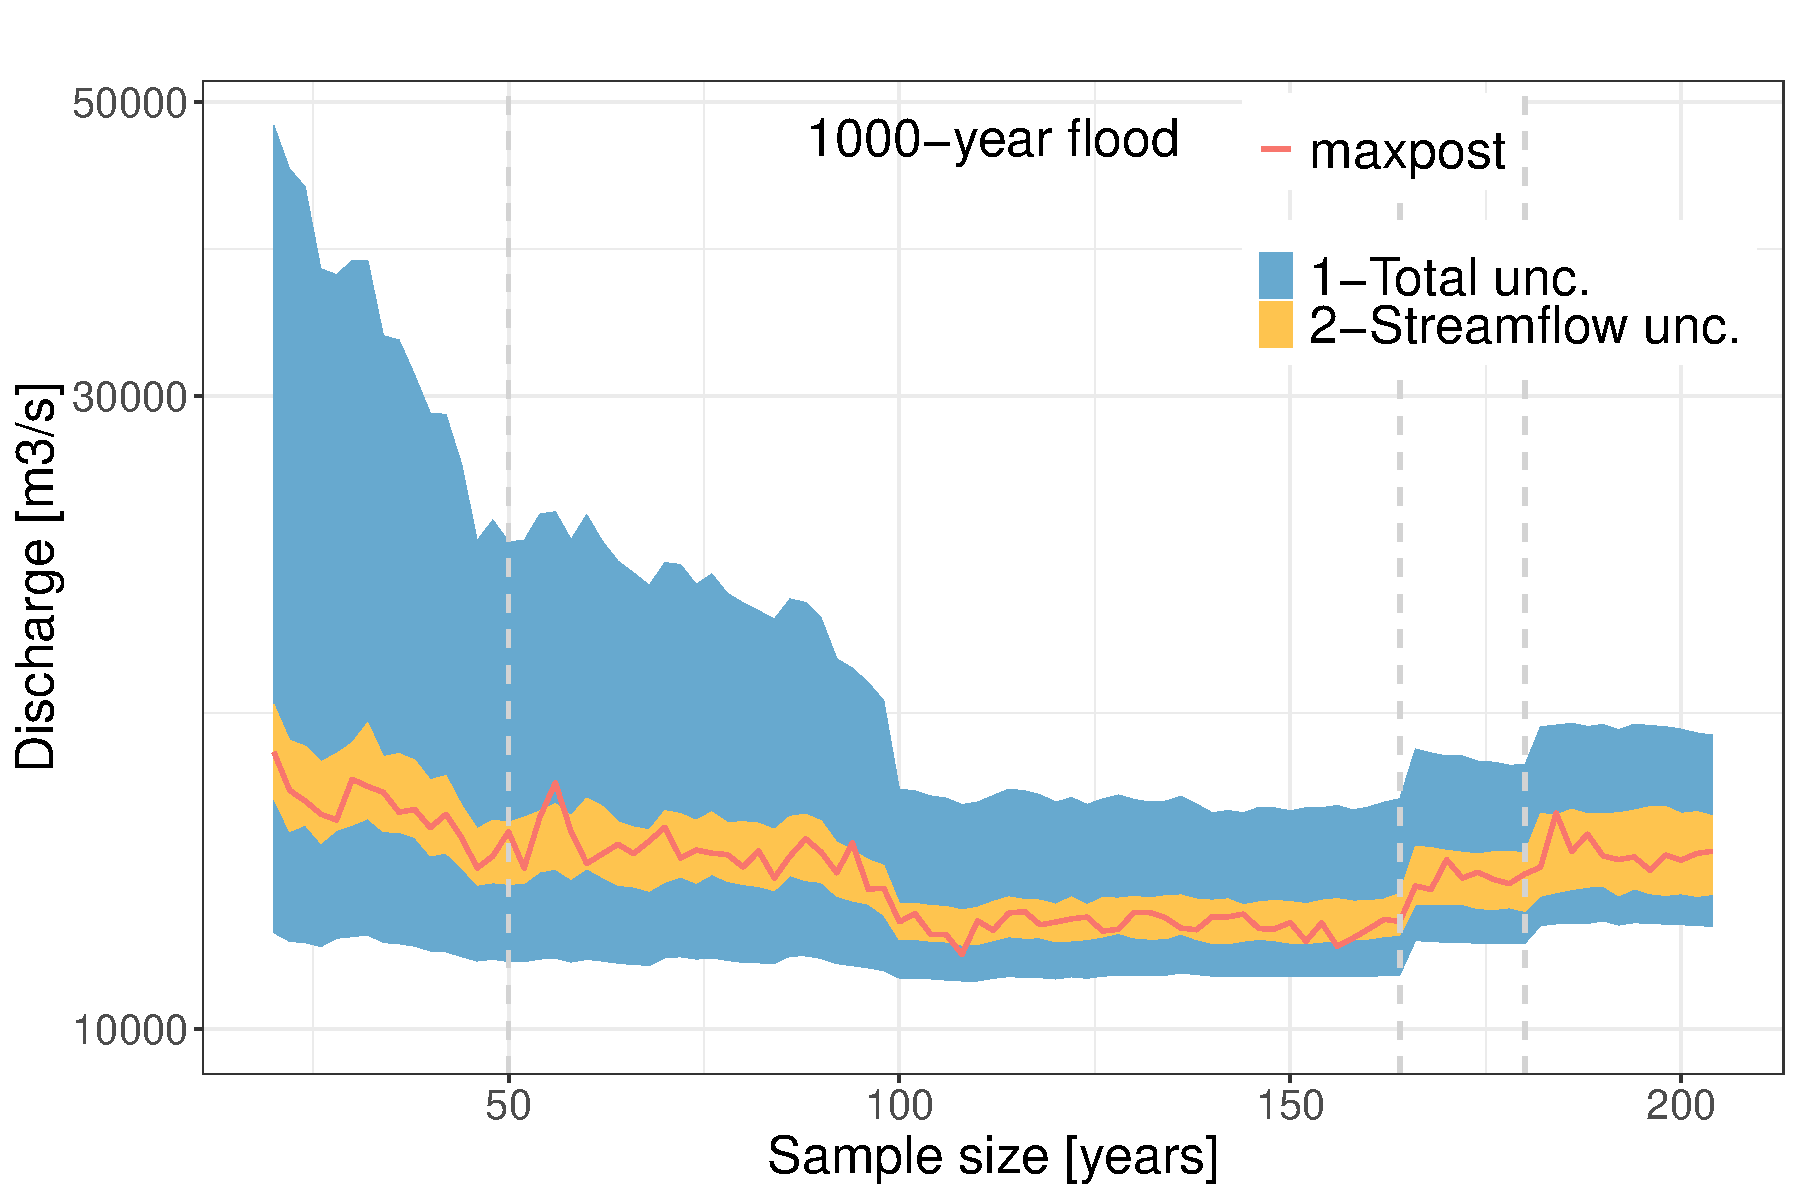
\includegraphics[width=\linewidth]{Figs/11d-Q1000SSize.pdf}
                \caption{}
                \label{subfig:SamplesQ1000}
            \end{subfigure}
            
            
        \caption{(a) Quantiles estimation for three return periods (10, 100 and 1000 years) for the four sample sizes (50, 100, 150 and 205 years). 95\% total uncertainty envelop is represented by the yellow error bars. 
        (b) Contribution of both sources of uncertainty to the total uncertainty for the four sample size cases. (c) GEV shape parameter distribution under streamflow and total uncertainty for the 4 sample sizes. (d) 1000-year flood estimations for various sample sizes from 20 to 205 years. The three grey dotted lines are representing important changes in the sample data, respectively: the change from Pont de Beaucaire to Beaucaire Restitution gauge, the inclusion of 1856 flood and the inclusion of 1840 flood to the sample.}
        \label{fig:Quantiles}
        \end{figure}

        \subsubsection{Sample size influence on quantiles uncertainty}
        
        With an exceptionally long sample at Beaucaire, the influence of sample size on flood quantiles estimation in a real case can be quantified, hence assessing the interest of using old hydrometric data when available. Four samples sizes are tested, taken as the last 50 years, 100 years, 150 years, and the largest available sample of 205 years. GEV distributions are estimated and the contribution of both sources of uncertainties is computed for each case, following section \ref{sec:STOODS} procedure.
        Total uncertainty is clearly reduced between the 50 years sample and the others samples for the three return periods: 10, 100 and 1000 years (figure \ref{subfig:BarplotQuantilesGev}). Surprisingly, for the 1000-year flood estimation, the total uncertainty is not reduced between the 100 and 205 years samples. This illustrates that the reduction of sampling uncertainty induced by increasing the sample size is compensated by the increased streamflow uncertainty when going back in time. 
        
        Figure \ref{subfig:UKplot4cases} is a good illustration of this phenomenon, showing the augmentation of the relative part of streamflow uncertainty when increasing the sample size. shape
        \paragraph{}
        The maxpost values of the 205 years sample in figure \ref{subfig:BarplotQuantilesGev} is higher than the 100 and 150 years samples, probably because of the inclusion of the two largest floods of the history in the 205 years sample (1840 and 1856 floods). Thus, without using those old hydrometric data although very uncertain (1816-1870), the 1000-year flood could have been 15\% lower in this specific case. The sample size impact on flood quantiles estimation is further explored in Figure \ref{subfig:SamplesQ1000}. The 1000-year flood (maxpost) and the part of both sources of uncertainties are estimated for several sample sizes, from 20 to 205 years, with a two-year step. A large reduction of sampling uncertainty (and of the total uncertainty as a consequence) appears between 20 and 100 years, along with the reduction of the maxpost value. Then, the maxpost 1000-flood value is almost constant between 100 and 160 years of sample size, until the inclusion of 1856 and 1840 floods that marks increases. The total uncertainty interval width is not much changed by those flood inclusions but the respective contribution of streamflow uncertainty appears more important.  
        
\section{Discussion and limitations of the procedure}

    \subsection{Strengths of the proposed approach}

    Even if sampling uncertainty is a major concern while conducting FFA, (systematic) historical hydrometric data is often forgotten. The laborious process to gather data and the concerns about its reliability may be the potential reasons of this oversight. The proposed approach is allowing a complete decomposition of the uncertainty trough the FFA chain. Uncertainties are propagated from stage to extreme quantiles. A similar approach have been proposed by \citet{steinbakk_propagation_2016}, who combined a Bayesian multi-segment rating curve model and FFA. However, the latter is not adapted to century-long series because stage measurements, gaugings and remnant rating curve uncertainties have been neglected. This could lead to the underestimation of extreme quantiles uncertainty. The proposed approach is merging recent works on streamflow uncertainty estimation (\citet{horner_impact_2018}; \citet{mansanarez_shift_2019}) and rating changes detection \citep{darienzo_detection_2021}), allowing an end-to-end uncertainty propagation, extended up to FFA. A particular attention is given to stage uncertainty, with the consideration of 5 major sources of errors including measurement frequency error that is often omitted. Thus, the contribution of the different sources of uncertainty to flood quantiles uncertainty is calculated. With the availability of a 205 years long streamflow series at Beaucaire, FFA uncertainty for different sample sizes is explored. \citet{petersen-overleir_accounting_2009} and \citet{steinbakk_propagation_2016} highlighted that considering rating curve uncertainty in FFA is enlarging the extreme quantiles estimates. We show similar results when considering not only rating curve uncertainty, but a larger number of uncertainty sources. We concluded that the contribution of both streamflow and sampling uncertainties is varying with sample size (\ref{subfig:UKplot4cases}). Sampling uncertainty is dominant for 50 and 100 years samples, for which the streamflow uncertainty is relatively small. The sampling uncertainty reduction when increasing sample size is offset by the increase of streamflow uncertainty when considering older and thus more uncertain floods. Although the respective contribution of both sources of uncertainty on the extreme quantiles are changing, the width of the uncertainty interval is not changing much from 100 to 205 years samples \ref{subfig:BarplotQuantilesGev}. However, in this case study, as the two largest floods of the gauge known history occurred during the first 50 years of records, the maxpost value of extreme quantiles is increased by 15\% when considering 205 years rather than 150 or 100 years (\ref{subfig:SamplesQ1000}). Therefore, not considering the full 205 years sample could lead to a different estimation of the flood hazard. 
    
    
    \subsection{Limitations and potential improvements}
    \paragraph{}
    The streamflow uncertainty analysis procedure proposed in this work is affected by several limitations. For simplicity purposes, gaugings stage uncertainty is assumed negligible, which is inconsistent with the consideration of stage measurement errors of section \ref{sec:StageErr}. \citet{horner_impact_2018} proposed a model that accounts for this source of uncertainty in a streamflow uncertainty propagation procedure.  
    \paragraph{}
    The gauging segmentation model proposed by \citet{darienzo_detection_2021} is an efficient tool to detect change points in the stage/discharge relationship, but it is constrained to its limit when dealing with old gauges for which gaugings are often scarce. One of the advantages of this approach is that it provides the probability density function (pdf) of the rating shifts dates in contrast to fix dates. This allows to select a date within the pdf according to the operator expertise, but this task is dubious when very few information are available about rating changes and channel morphology. Additional tests could be used to investigate about stage/discharge relationship, such as the analysis of flood recessions proposed in \citet{darienzo_detection_2021-1}
    \paragraph{}
    Another limitation of the method comes from the elicitation of hydraulic priors in historical context, for which information about hydraulic configuration is scarce. This lack of knowledge is impacting when considering gauges where works inside the main channel were frequent. The Rhône River is part of those, even if it holds the interest of many historians who retrieved many pieces of hydraulic and morphological data. 
    \paragraph{}
    Another drawback comes from the fact that, for simplification purposes, we considered the days of annual maximum discharge as the days of annual maximum stage. For a given year, if $h_{j} > h_{k}$, it's not guaranteed that $Q_{j} > Q_{k}$ if there is an important rating curve change during this given year. 
    \paragraph{}
    The BaRatin \citep{lecoz_quantification_2014} based propagation model choice may have an important impact on uncertainty estimation, as the seven rating curve uncertainty estimation methods compared by \citet{kiang_comparison_2018} concluded in a very large differences in uncertainty intervals.
    \paragraph{}
    GEV distribution have been chosen because of its flexibility to describe several tail behaviours. However, many other distributions, as legitimate as GEV in our case-study, might give different results. 
    \paragraph{}
    Shape parameter is of great importance as it determines the tail behaviour of the distribution. Several regional or local-regional methods have been proposed to reduce the uncertainty around shape parameter estimation. \citet{renard_data-based_2013} have proposed a framework to compare those different possibilities. They concluded in particular that the best results were given by local-regional approach, as proposed by \citet{ribatet_regional_2007}. This could be a source of improvement, but the definition of regional approach could be difficult for a catchment as large as the Rhône River at Beaucaire.
    \paragraph{}
    It could be interesting to evaluate the procedure on several different gauges to have a better estimation of the added value of long streamflow series in FFA. The results of this work based on one station may not be accurate for every gauge with historical hydrometric data.  
    \paragraph{}
    Although the homogeneity of AMAX discharges have been checked prior to FFA, the underlying assumption of stationarity required for FFA may have been corrupted by anthropogenic climate change, as described by \citet{milly_stationarity_2008}. Trends have been identified in several climatic regions of Europe \citep{hall_understanding_2014} and France \citep{renard_regional_2008}, but no general change was found. The Rhône River catchment at Beaucaire is at the crossroad of several climatic regions for which trends are opposed. Also, \citet{madsen_floodfreq_2013} underlined that no particular guideline for climate change adjustment factors on design floods are given in France.
    \paragraph{}
    Finally, promising improvements could come from the further valorization of historical data by investigating floods evidences before systematic stage measurements. Various procedures have been developed in the literature, through the use of perception threshold and censored data as summarized by \citet{kjeldsen_documentary_2014} or \citet{brazdil_historical_2006}. Applications of this kind of approach have emerged in Europe, including France (\citet{naulet_flood_2005}; \citet{lang_extrapolation_2010}; \citet{neppel_flood_2010}; \citet{payrastre_usefulness_2011}) and could be interesting for the Lower-Rhône Valley for which many climatic and flood evidences have been gathered (see \citet{pichard_sept_2014} and \citet{pichard_hydro-climatology_2017}).
    
    
\section{Conclusion}
    \paragraph{}
    This paper presents a general framework for flood frequency analysis accounting for uncertainties in the specific case of long discharge series. First, several methods allowing to estimate and propagate the different sources of streamflow uncertainty have been chained: stage uncertainty (with a particular attention on measurement frequency error), rating changes and multiperiod rating curves estimation methods have been considered. The several uncertainties have been propagated towards streamflow series, allowing to access to the different contribution of each source in the total streamflow uncertainty. Then, streamflow uncertainties have been propagated through FFA, allowing to estimate the relative contribution of sampling and streamflow uncertainties in the extreme quantiles. 
    \paragraph{}
    The procedure have been applied to the Rhône River at Beaucaire, where systematic stage measurements are available since 1816. The size of this exceptional series allowed to test the impact of sample size on extreme quantiles uncertainties by using successively 50, 100, 150 and the full 205 years available. First, the total uncertainty appears to decrease when sample size increases, thank to sample uncertainty reduction. This decrease is particularly important between 50 and 100 years sample sizes, but less important above 100 years samples. Also, while the size of the uncertainty interval is not much changing when increasing sample size above 100 years, the most probable values (maxpost) were increasing because the two largest floods of the gauge occurred during the first 50 years. Not considering those floods could have resulted in a much different estimation of flood quantiles. This highlights the added value of long streamflow series for FFA and the importance of accounting for streamflow uncertainties, as almost 50\% of the quantiles uncertainties is coming from streamflow for the 205 years long sample.

\section{Acknowledgements}

H2O + ENS Lyon + CNR ?

\newpage
\printbibliography
\newpage 

\section{Annexes}

    \subsection{Rating curve hydraulic priors}
        
        \begin{table}[h!]
            \begin{tabular}{|l|l|l|l|l|}
            \firsthline
            Physical param. & Meaning & Prior & Inferred param. & Prior\\
            \hline
            \multicolumn{5}{|l|}{\textbf{Control 1: main channel}} \\
            $b_1 [m]$      &   Offset              &  $\mathcal{N}(-4,0.5)$   &     $b_1 [m]$    &  $\mathcal{N}(-4,0.5)$ \\
            \hline
            $B_1 [m]$     &   Channel width   &  $\mathcal{LN}(ln(300),0.16)$&$a_1 [m^{3/2}/s]$  & $\mathcal{LN}(ln(128.6),1.8.10^{-2})$\\
            $K_1 [m^{1/3}/s]$&   Strickler coeff. &  $\mathcal{LN}(ln(35),0.14)$    &                &                     \\
            $S_1 [m/m]$     &   Bed slope        &  $\mathcal{LN}(ln(1.5.10^{-4}),0.55)$         &                &  \\
            \hline
            $c_1 [-]$     &   Exponent            &  $\mathcal{N}(5/3,0.025)$&     $c_1 [-]$     &$\mathcal{N}(5/3,0.025)$\\
            \hline
            \multicolumn{5}{|l|}{\textbf{Control 2: floodway}} \\
            %\hline
            $b_2 [m]$     &   Offset              &  $\mathcal{N}(1.5,0.5)$   &     $b_2 [m]$   &  $\mathcal{N}(1.5,0.5)$ \\
            \hline
            $B_2 [m]$     &   Channel width   &  $\mathcal{LN}(ln(500),0.1)$  &   $a_2 [m^{3/2}/s]$&  $\mathcal{LN}(ln(241.9),1.10^{-2})$\\
            $K_2 [m^{1/3}/s]$&   Strickler coeff. &  $\mathcal{LN}(ln(30),0.16)$    &                 &                     \\
            $S_2 [m/m]$     &   Bed slope        &   $\mathcal{LN}(ln(2.6.10^{-4}),0.34)$        &                &\\
            \hline
            $c_2 [-]$     &   Exponent           &  $\mathcal{N}(5/3,0.025)$&     $c_2 [-]$    &$\mathcal{N}(5/3,0.025)$\\
            \hline
            \multicolumn{5}{|l|}{\textbf{Structural uncertainty parameters}} \\
            %\hline
            $\gamma_{1} [m^{3}/s]$ & Intercept & $\mathcal{U}(0,1000)$ & $\gamma_{1} [m^{3}/s]$ & $\mathcal{U}(0,1000)$\\
            $\gamma_{2} [-]$ & Slope & $\mathcal{U}(0,100)$ & $\gamma_{2} [-]$ &$\mathcal{U}(0,100)$  \\
            \hline
            \multicolumn{5}{|l|}{\textbf{Multiperiod RC parameters}} \\
            $\delta l [m]$     &   Local change    &  $\mathcal{N}(0,0.3)$&      $\delta l [m]$     &$\mathcal{N}(0,0.3)$\\
            $\delta g [m]$     &   Global change       &  $\mathcal{N}(0,0.3)$&      $\delta g [m]$     &$\mathcal{N}(0,0.3)$\\
            \lasthline
            \end{tabular} 
            \caption{Priors elicitation for Pont de Beaucaire. $\mathcal{U}$ stands for continuous uniform distribution, $\mathcal{N}$ for Normal distribution and $\mathcal{LN}$ for Log Normal distribution}
            \label{tab:PriorPt}
       \end{table}
       
    % \newpage 
    % \subsection{Beaucaire Restitution hydraulic priors}
    
        \begin{table}[h!]
            \begin{tabular}{|l|l|l|l|l|}
            \firsthline
            Physical param. & Meaning & Prior & Inferred param. & Prior\\
            \hline
            \multicolumn{5}{|l|}{\textbf{Control 1: Low flows channel}} \\
            $b_1 [m]$      &   Offset              &  $\mathcal{N}(-5,0.5)$   &     $b_1 [m]$    &  $\mathcal{N}(-5,0.5)$ \\
            \hline
            $B_1 [m]$     &   Channel width   &  $\mathcal{LN}(ln(200),0.42)$&$a_1 [m^{3/2}/s]$  & $\mathcal{LN}(ln(49.50),3.2.10^{-2})$\\
            $K_1 [m^{1/3}/s]$&   Strickler coeff. &  $\mathcal{LN}(ln(35),0.14)$    &              &                     \\
            $S_1 [m/m]$     &   Bed slope        &  $\mathcal{LN}(ln(5.10^{-5}),0.20)$         &                  & \\
            \hline
            $c_1 [-]$     &   Exponent            &  $\mathcal{N}(5/3,0.025)$&     $c_1 [-]$     &$\mathcal{N}(5/3,0.025)$\\
            \hline
            \multicolumn{5}{|l|}{\textbf{Control 2: Main channel}} \\
            $b_1 [m]$      &   Offset              &  $\mathcal{N}(0,0.5)$   &     $b_1 [m]$    &  $\mathcal{N}(0,0.5)$ \\
            \hline
            $B_1 [m]$     &   Channel width   &  $\mathcal{LN}(ln(300),0.32)$& $a_2 [m^{3/2}/s]$  & $\mathcal{LN}(ln(148.49),2.4.10^{-2})$\\
            $K_1 [m^{1/3}/s]$&   Strickler coeff. &  $\mathcal{LN}(ln(35),0.14)$    &              &                     \\
            $S_1 [m/m]$     &   Bed slope        &  $\mathcal{LN}(ln(2.10^{-4}),0.25)$         &              & \\
            \hline
            $c_1 [-]$     &   Exponent            &  $\mathcal{N}(5/3,0.025)$&     $c_2 [-]$     &$\mathcal{N}(5/3,0.025)$\\
            \hline
            \multicolumn{5}{|l|}{\textbf{Control 3: Floodway}} \\
            %\hline
            $b_3 [m]$     &   Offset              &  $\mathcal{N}(8,0.5)$   &     $b_3 [m]$   &  $\mathcal{N}(8,0.5)$ \\
            \hline
            $B_3 [m]$     &   Channel width   &  $\mathcal{LN}(ln(200),0.47)$  &   $a_3 [m^{3/2}/s]$ &  $\mathcal{LN}(ln(241.9),1.10^{-2})$\\
            $K_3 [m^{1/3}/s]$&   Strickler coeff. &  $\mathcal{LN}(ln(25),0.20)$    &              &                     \\
            $S_3 [m/m]$     &   Bed slope        &   $\mathcal{LN}(ln(2.4.10^{-4}),0.21)$        &                      &\\
            \hline
            $c_3 [-]$     &   Exponent           &  $\mathcal{N}(5/3,0.025)$&     $c_3 [-]$    &$\mathcal{N}(5/3,0.025)$\\
            \hline
            \multicolumn{5}{|l|}{\textbf{Structural uncertainty parameters}} \\
            %\hline
            $\gamma_{1} [m^{3}/s]$ & Intercept & $\mathcal{U}(0,1000)$ & $\gamma_{1} [m^{3}/s]$ & $\mathcal{U}(0,1000)$\\
            $\gamma_{2} [-]$ & Slope & $\mathcal{U}(0,100)$ & $\gamma_{2} [-]$ &$\mathcal{U}(0,100)$  \\
            \hline
            \multicolumn{5}{|l|}{\textbf{Multiperiod RC parameters}} \\
            $\delta l [m]$     &   Local change    &  $\mathcal{N}(0,0.8)$&      $\delta l [m]$     &$\mathcal{N}(0,0.8)$\\
            $\delta g [m]$     &   Global change       &  $\mathcal{N}(0,0.3)$&      $\delta g [m]$     &$\mathcal{N}(0,0.3)$\\
            \lasthline
            \end{tabular} 
            \caption{Priors elicitation for Beaucaire reconstitution. $\mathcal{U}$ stands for continuous uniform distribution, $\mathcal{N}$ for Normal distribution and $\mathcal{LN}$ for Log Normal distribution}
            \label{tab:PriorRestit}
       \end{table}
       
       \newpage
       
       \subsection{Gaugings segmentation detailed results}
    
    \begin{center}
        \begin{table}[h!]
        \centering
            \begin{tabular}{|m{3cm}|m{3cm}|m{3cm}|m{2cm}|m{2cm}|}
                \firsthline
                \textbf{Maxpost shift time}  &  \textbf{Largest flood within \textit{post. pdf}} &  \textbf{Final choice} & \textbf{Period number} & \textbf{Number of gaugings}  \\
                \hline
                No gaugings     &      No gaugings   &   1840-11-02 & 1 & 0 \\
                \hline
                1860-02-20     &       1856-06-01  &   1856-06-01   & 2 & 4 \\
                \hline
                1887-05-11     &       1886-10-29  &   1886-10-29   & 3 & 6\\
                \hline
                1910-11-21     &       1910-12-09  &   1910-12-09  & 4 & 58 \\
                \hline
                1921-06-22     &       1935-11-14  &   1935-11-14   & 6 & 22 \\
                \hline
                1954-08-08    &       1951-11-23  &   1951-11-23   & 6 & 1\\
                \hline
                1954-03-30     &       1955-01-23  &   1955-01-23   & 7 & 3 \\
                \hline
                1963-03-23     &       1963-11-08  &   1963-11-08   & 8 & 91 \\
                \hline
                1967-01-31     &       1967-01-31  &   1967-01-31  & 9 & 43\\
                \hline
                1967-12-31      &       End of stage series & End of stage series & 10 & 5\\
                \hline
                \hline
                1975-02-06     &       1976-11-11  &   1976-11-11 & 1 & 3\\
                \hline
                1994-06-10     &       1994-01-08  &   1994-01-08   & 2 & 122 \\
                \hline
                2003-08-05     &       2002-11-27  &   2002-11-27  & 3 & 65 \\
                \hline
                2003-10-09     &       2003-12-04  &   2003-12-04   & 4 & 17 \\
                \hline
                2004-02-16     &       2003-12-04  &   No shift   & X & X \\
                \hline
                2004-07-15     &       2003-12-04  &   2004-07-15   & 5 & 1 \\
                \hline
                2004-12-02     &       2004-12-02  &   2004-12-02   & 6 & 2 \\
                \hline
                2005-07-03     &       2004-12-02  &   No shift  & X & X \\
                \hline
                2005-12-24     &       2003-12-04  &   2005-12-24  & 7 & 14 \\
                \hline
                2008-06-28     &       2003-12-04  &   2008-06-28    & 8 & 28 \\
                \hline
                2009-10-20     &       2003-12-04  &   2009-10-20   & 9 & 7 \\
                \hline
                2016-11-21     &       2016-11-22  &   2016-11-22  & 10 & 26 \\
                \hline
                2019-02-11     &       2018-11-24  &   No shift   & X & X \\
                \hline
                2020-01-01     &      End of stage series  &   End of stage series  & 11 & 11\\
                \lasthline
            \end{tabular}
            
            \caption{Beaucaire rating shifts dates}
            \label{tab:ShiftDates}
        \end{table}
    \end{center}
    
    
    %tab to be removed
    % \begin{center}
    %     \begin{table}
    %     \centering
    %         \begin{tabular}[h]{|m{4cm}|m{4cm}|m{4cm}|}
    %             \firsthline
    %             \textbf{Maximum \textit{post. pdf}}  &  \textbf{Largest flood within \textit{post. pdf}} &  \textbf{Final choice}    \\
    %             \hline
    %             1975-02-06     &       1976-11-11  &   1976-11-11 \\
    %             \hline
    %             1994-06-10     &       1994-01-08  &   1994-01-08   \\
    %             \hline
    %             2003-08-05     &       2002-11-27  &   2002-11-27   \\
    %             \hline
    %             2003-10-09     &       2003-12-04  &   2003-12-04   \\
    %             \hline
    %             2004-02-16     &       2003-12-04  &   X   \\
    %             \hline
    %             2004-07-15     &       X  &   2004-07-15   \\
    %             \hline
    %             2004-12-02     &       X  &   2004-12-02   \\
    %             \hline
    %             2005-07-03     &       X  &   X   \\
    %             \hline
    %             2005-12-24     &       X  &   2005-12-24   \\
    %             \hline
    %             2008-06-28     &       X  &   2008-06-28   \\
    %             \hline
    %             2009-10-20     &       X  &   2009-10-20   \\
    %             \hline
    %             2016-11-21     &       2016-11-22  &   2016-11-22   \\
    %             \hline
    %             2019-02-11     &       X  &   X   \\
    %             \lasthline
    %         \end{tabular}
            
    %         \caption{Beaucaire Restitution rating shifts dates, floods within posterior \textit{pdf} are indicated when larger than the 10 years return period discharge.}
    %         \label{tab:ShiftDatesRestit}
    %     \end{table}
    % \end{center}

    

\end{document}

